%%%%%%%%%%%%%%%%%%%%%%%%%%%%%%%%%%%%%%%%%12pt: grandezza carattere
                                        %a4paper: formato a4
                                        %openright: apre i capitoli a destra
                                        %twoside: serve per fare un
                                        %   documento fronteretro
                                        %report: stile tesi (oppure book)
\documentclass[12pt,a4paper,openright,twoside]{report}

\usepackage[italian]{babel}
\usepackage[utf8]{inputenc}
\usepackage{fancyhdr}
\usepackage{indentfirst}
\usepackage{graphicx}
\usepackage{wrapfig}
\usepackage{caption}
\usepackage{subcaption}
\usepackage{newlfont}
\usepackage{amssymb}
\usepackage{amsmath}
\usepackage{listings}
\usepackage{color}
\usepackage[hyphenbreaks]{breakurl}
\usepackage[hyphens]{url}
\usepackage{longtable}
\usepackage{colortbl}
\usepackage{fancyvrb}
\usepackage{multirow}
\usepackage[font={footnotesize}]{caption}

\hfuzz=30pt
\vfuzz=30pt
\hbadness=10000
\vbadness=\maxdimen

\sloppy

\definecolor{gray}{rgb}{0.4,0.4,0.4}
\definecolor{darkblue}{rgb}{0.0,0.0,0.6}
\definecolor{cyan}{rgb}{0.0,0.6,0.6}
\definecolor{lightcyan}{rgb}{0,1,1}
\definecolor{yellow}{rgb}{1,1,0}
\definecolor{lightyellow}{rgb}{1,1,0.6}

\renewcommand{\lstlistingname}{Listato}
\lstset{
  inputencoding=ansinew,
  breaklines=true,
  basicstyle=\ttfamily\scriptsize,
  columns=fullflexible,
  showstringspaces=false,
  commentstyle=\color{gray}\upshape,
  literate=%
  {à}{{\`a}}1
  {ò}{{\`o}}1
  {ö}{{\"o}}1
}
\lstdefinelanguage{XML}
{
  morestring=[b]",
  morestring=[s]{>}{<},
  morecomment=[s]{<?}{?>},
  stringstyle=\color{black},
  identifierstyle=\color{darkblue},
  keywordstyle=\color{cyan},
  morekeywords={xmlns,version,type}
}


\def\signed #1{{\leavevmode\unskip\nobreak\hfil\penalty50\hskip2em
  \hbox{}\nobreak\hfil(#1)%
  \parfillskip=0pt \finalhyphendemerits=0 \endgraf}}

\newsavebox\mybox
\newenvironment{aquote}[1]
  {\savebox\mybox{#1}\begin{quote}}
  {\signed{\usebox\mybox}\end{quote}}

\oddsidemargin=30pt \evensidemargin=20pt
\hyphenation{sil-la-ba-zio-ne pa-ren-te-si}

\pagestyle{fancy}\addtolength{\headwidth}{20pt}\addtolength{\headheight}{15pt}
\renewcommand{\chaptermark}[1]{\markboth{\thechapter.\ #1}{}}
\renewcommand{\sectionmark}[1]{\markright{\thesection \ #1}{}}
\rhead[\fancyplain{}{\bfseries\leftmark}]{\fancyplain{}{\bfseries\thepage}}
\cfoot{}

\linespread{1.3}

\begin{document}
\begin{titlepage}
\thispagestyle{empty}
\topmargin=6.5cm
\raggedleft
\large
\em
A papà e mamma.
\newpage
\clearpage{\pagestyle{empty}\cleardoublepage}
\end{titlepage}

\pagenumbering{roman}

% table of contents
\tableofcontents
\rhead[\fancyplain{}{\bfseries\leftmark}]{\fancyplain{}{\bfseries\thepage}}
\lhead[\fancyplain{}{\bfseries\thepage}]{\fancyplain{}{\bfseries
INDICE}}
\clearpage{\pagestyle{empty}\cleardoublepage}

% figures list
\listoffigures
\clearpage{\pagestyle{empty}\cleardoublepage}

%\lstlistoflistings
%\clearpage{\pagestyle{empty}\cleardoublepage}

% tables list
\listoftables
\clearpage{\pagestyle{empty}\cleardoublepage}

\lhead[\fancyplain{}{\bfseries\thepage}]{\fancyplain{}{\bfseries\rightmark}}
\pagenumbering{arabic}

\chapter{Introduzione}

La gestione dell'informatizzazione degli archivi riguardanti beni culturali e eredità culturale è da tempo argomento di discussione critico sia per gli archivisti che per gli informatici.

Da quando i computer sono diventati parte della vita e delle tecnologie utilizzate quotidianamente, la sfida, in questo come in altri campi, è quella di ``informatizzare'' gli storici cataloghi cartacei, ovvero trasformare schedari, libri mastri e altre forme di catalogazione in dati gestibili da una macchina.

Tale sfida risulta ancora più difficile se si aggiunge, oltre alla indispensabile elaborazione e trascrittura dei dati, l'analisi, la scelta e la modellazione di formati fruibili e interoperabili tra di loro, la creazione cioè di standard che possano essere di riferimento alle varie entità deputate alla conservazione di tali dati; per dare una soluzione a questo problema, nel tempo si sono costituiti gruppi più o meno autorevoli e ognuno ha prodotto dei modelli più o meno utilizzabili e allo stesso modo più o meno diffusi e applicati.

Oltre a questa frammentazione, normalmente a livello nazionale, i modelli definiti soffrono spesso, in particolare i più datati, di una significativa aderenza al modello precedente, ovvero la scheda cartacea, con la conseguente definizione di standard molto ricchi in dettaglio ma poveri in profondità e riferimenti incrociati: è il caso, ad esempio nel mondo bibliografico, dei vari standard \emph{MARC}\footnote{\url{http://www.loc.gov/marc/}} nazionali e del tentativo di unificarli con il modello \emph{Unimarc}\footnote{\url{http://it.wikipedia.org/wiki/UNIMARC}}.

Lo sforzo è quindi quello di ripensare i modelli esistenti in un'ottica di unificazione, in particolare grazie all'evoluzione del web e all'imponente crescita dei LOD (vedi~\ref{sec:semantic-web}), per riconvertire le informazioni in dati collegati e disponibili in rete.

In questa relazione verrà esaminato un caso concreto di questa esigenza di riconversione e apertura: l'archivio fotografico della \emph{Fondazione Federico Zeri}, una delle più grandi collezioni di fotografie di opere d'arte esistenti a livello mondiale.

Per l'informatizzazione e la catalogazione dell'eredità culturale, in Italia il Ministero dei Beni Culturali ha istituito un gruppo, l'\emph{Istituto Centrale per il Catalogo e la Documentazione} (ICCD) il quale, tra le altre cose, ha prodotto una serie di normative e modelli\footnote{\url{http://www.iccd.beniculturali.it/index.php?it/204/normative}} da utilizzare a seconda della natura del bene in questione.

Il modello per la fotografia è chiamato \emph{Scheda F} e contiene un ricco insieme di campi per la descrizione degli oggetti fotografici, pur soffrendo delle limitazioni viste poc'anzi. Tale modello è quello utilizzato dalla \emph{Fondazione Federico Zeri} per il catalogo dell'importante archivio fotografico raccolto da Zeri durante la sua carriera; le singole schede sono disponibili per la visualizzazione, grazie anche all'imponente lavoro di digitalizzazione, online.

L'obiettivo del progetto è portare tale disponibilità di informazione ad un livello successivo, standard, fruibile e interoperabile tramite la conversione dell'attuale base di dati nel dominio di Linked Open Data, strutturando il modello in modo che possa essere da esempio per progetti di conversione di archivi analoghi.

È stata quindi effettuata un'analisi approfondita sulla struttura dei dati attuale e sulle ontologie disponibili e utilizzate al momento nel campo dell'eredità culturale, che ha permesso di formulare una mappatura delle informazioni catalografiche in statement RDF e la modellazione di un'ontologia specifica definita \emph{F Entry Ontology} (cap.~\ref{chap:mapping}).

Di rilevanza fondamentale durante la fase di analisi e modellazione è stata la necessità di avere una mappatura che permettesse il maggior grado possibile di automazione, vista l'imponenza degli archivi di partenza.

L'effettiva implementazione (cap.~\ref{chap:implementation}) è stata realizzata in un set di script Python tenendo presente i requisiti di modularità, flessibilità e riuso del codice.

\clearpage{\pagestyle{empty}\cleardoublepage}

\chapter{I Linked Open Data in ambito archivistico}

\section{L'eredità culturale: dai graffiti ad oggi}

Tramandare le conoscenze e le esperienze dal vecchio al giovane è un'impresa che ha coinvolto l'uomo fin dal primo segno tracciato sulla parete della caverna che gli dava riparo.\\
L'importanza di lasciare in eredità il sapere accumulato così che chi fosse venuto dopo avesse potuto comprenderlo, rettificarlo e migliorarlo è stata fondamentale durante tutta l'evoluzione culturale dell'uomo, permettendo continue applicazioni, riusi e affinamenti di un corpus enciclopedico sempre più vasto e utile.

In parallelo al miglioramento del sapere in sé è avvenuto un miglioramento dei mezzi per la trasmissione di quest'ultimo, in termini di comprensibilità, durabilità e praticità. Con i racconti omerici e i Vangeli del tutto sensibili a riletture e deformazioni a causa della trasmissione orale, nacquero le immense biblioteche monacensi; la stampa seriale superò il limite della scarsa diffusione e accessibilità di queste ultime. La fotografia e la microfotografia permisero una riproducibilità più rapida ed affidabile, i computer la migliorarono ulteriormente assieme alla risoluzione dei problemi di conservazione.

\subsection{Una rete multiforme}
Ai giorni nostri, le reti di computer (e più nello specifico, Internet) hanno permesso una maggiore pervasività e disponibilità dell'informazione, accessibile ormai a chiunque in tempi pressoché istantanei, per quanto riguarda sia la fruizione sia la creazione di contenuti e conoscenze.\\
Tale velocità e apertura è allo stesso tempo il suo punto di forza e di debolezza: i problemi attuali sono infatti l'autorevolezza (e il conseguente ``rumore digitale'') ma soprattutto la definizione di formati standard comuni per definizione, fruizione e riuso delle informazioni.

\subsection{Il web semantico}\label{sec:semantic-web}
Il potere principale della rete è quello, appunto, di essere una rete, ovvero di poter interconnettere pezzi (\emph{risorse}) di informazione presenti in ``luoghi'' diversi tra di loro e permettere di seguire un percorso in base ai collegamenti propri della risorsa che stiamo esaminando, fin dalla prima formulazione dello standard HTML.\\
Oggi assistiamo ad una evoluzione (fig.~\ref{fig:web_evolution}) del modo di fruire la rete nell'interconnessione non solo dei documenti, ai quali era inizialmente limitato il web, ma anche degli utenti (Web 2.0); tale evoluzione sta procedendo nella direzione del \emph{web semantico}, dove tutto (documenti, utenti, concetti, persone, etc.) è considerato una \emph{risorsa} ed è collegato e collegabile con altre risorse, idealmente racchiudendo tramite tale struttura a grafo tutta l'informazione umana (Web 3.0\footnote{Il nome \emph{Web 3.0} è stato usato inizialmente da Jeffrey Zeldman \cite{30} e quindi ripreso da Tim Berners-Lee \cite{31} in riferimento ad un web più ``intelligente'' che comprenda, oltre all'informazione aperta e strutturata, anche connessione onnipresente, formati aperti, dati nella nuvola e più in generale l'abbandono del legame alla ``fisicità'' degli strumenti per l'accesso alla rete stessa}).

\begin{figure}[ht!]
	\centering
	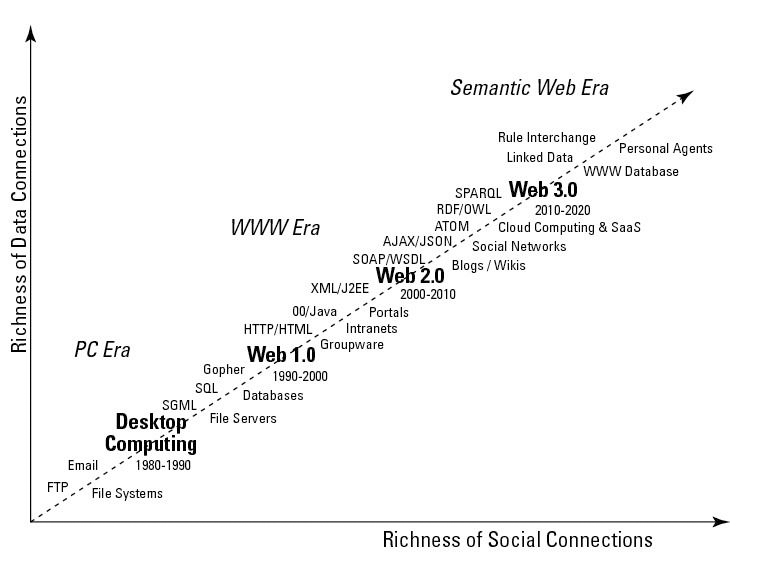
\includegraphics[width=90mm]{images/Four-major-waves-of-Web-evolution.jpg}
	\caption{Evoluzione del web, in \cite{1}}
	\label{fig:web_evolution}
\end{figure}

Il web semantico si concentra quindi:
\begin{quote}
sui dati e sul formato di rappresentazione degli stessi, sul linguaggio e su come i dati si relazionano agli oggetti del mondo reale, il che permette ad una persona o ad una macchina di seguire un percorso tra dati di natura diversa che non sia attraverso dei cavi bensì tramite collegamenti semantici.\cite{2}
\end{quote}

\subsection{Giant Global Graph e Linked Open Data}
Questo spostamento d'accento dal documento in sé alla relazione che intercorre con altre risorse è stato sottolineato da Tim Berners-Lee (co-inventore del World Wide Web) nel suo articolo \emph{Giant Global Graph} \cite{3}, evidenziando come il salire sopra al livello del singolo documento permetta il riuso dell'informazione\footnote{\url{https://www.youtube.com/watch?v=OM6XIICm_qo}}.

Il concetto di \emph{Linked Open Data} (LOD) implementa il web semantico permettendo la creazione di relazioni (\emph{link}) tra risorse (\emph{data}) e rendendole fruibili e accessibili (\emph{open}) così da favorirne e incoraggiarne l'uso e il riuso.

Berners-Lee concettualizza i LOD definendo quattro regole:
\begin{enumerate}
\item Usate gli URI come nome per le cose.
\item Usate URI HTTP così che gli utenti possano recuperarli.
\item Quando un utente accede ad un URI fornite informazioni utili attraverso gli standard (RDF, SPARQL).
\item Includete collegamenti ad altri URI così che gli utenti possano scoprire più cose.
\end{enumerate}
Se una sola di queste regole è disattesa, secondo Berners-Lee non si può parlare di LOD. \cite{4}

La rappresentazione dei dati, dovendo essere comprensibile tanto all'uomo quando alla macchina, si è fatta forte del costrutto più basilare del linguaggio, ovvero la struttura \verb"soggetto-predicato-oggetto": lo standard per i LOD è infatti RDF\footnote{\url{http://it.wikipedia.org/wiki/Resource_Description_Framework}}, dove ogni relazione viene rappresentata per l'appunto da una tale tripla (chiamata \emph{statement}).\\
Ad esempio, nello statement \texttt{Federico Zeri è autore della fotografia \#231} abbiamo
\begin{itemize}
\item \verb"Federico Zeri" come soggetto
\item \verb"è autore di" come predicato
\item \verb"fotografia #231" come oggetto
\end{itemize}
Questa formulazione non fa assunzioni sul dominio del discorso e lascia pertanto completa libertà sulla formulazione degli statement che risultano comprensibili tanto dall'uomo quanto dalla macchina.

\section{I LOD per l'eredità culturale}

L'avvento dei LOD ha aperto un interessante campo di studio e ricerca in particolare per biblioteche, archivi e musei, costantemente alla ricerca  e alla sperimentazione di nuovi modi per rendere i dati disponibili, fruibili e riusabili dagli utenti \cite{5}. Lo sforzo da parte di queste istituzioni è sempre stato quello di conservare e migliorare la visione e revisione dei contenuti da parte di studiosi, ricercatori e utenti in genere; è quindi naturale che la possibilità di intercorrelare le informazioni diventi particolarmente appetibile.

\subsection{LOD e archivi}
L'introduzione di una nuova pratica o tecnologia comporta un normale periodo di ``rodaggio'' iniziale, spesso accompagnato da una frammentazione durante la definizione di uno o più standard da seguire.\\
Sebbene la curva di crescita dei LOD appaia decisamente ripida (fig.~\ref{fig:lod-cloud}) come evidenzia \cite{21}, coinvolgendo alcune delle più importanti organizzazioni a livello mondiale, moltissimi archivi ne restano ancora esclusi, principalmente per la mancanza di mezzi economici e tecnologici che riescano a convertire i database, pur dettagliati e articolati, in dataset aperti aderenti agli standard che caratterizzano la nuvola dei LOD.

\begin{figure}
    \centering
    \begin{subfigure}[b]{0.5\textwidth}
            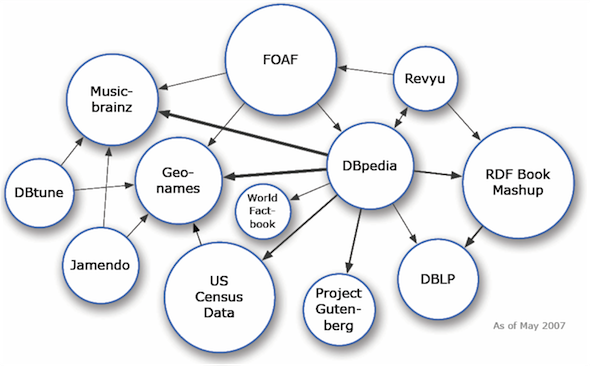
\includegraphics[width=\textwidth]{images/lod-cloud-2007.png}
            \caption{Maggio 2007}
            \label{fig:lod-cloud-2007}
    \end{subfigure}%
    ~ %add desired spacing between images, e. g. ~, \quad, \qquad, \hfill etc.
      %(or a blank line to force the subfigure onto a new line)
    \begin{subfigure}[b]{0.5\textwidth}
            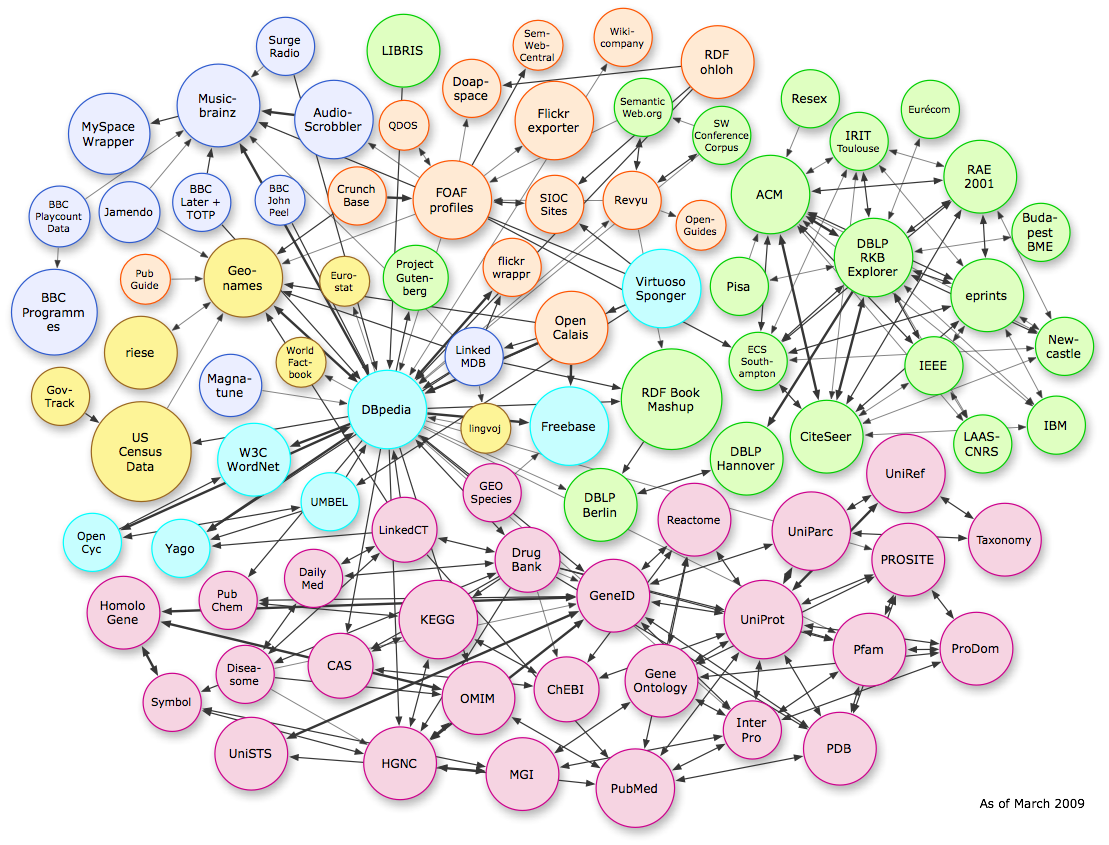
\includegraphics[width=\textwidth]{images/lod-cloud-2009.png}
            \caption{Marzo 2009}
            \label{fig:lod-cloud-2009}
    \end{subfigure}
    %add desired spacing between images, e. g. ~, \quad, \qquad, \hfill etc.
    %(or a blank line to force the subfigure onto a new line)

    \begin{subfigure}[b]{\textwidth}
            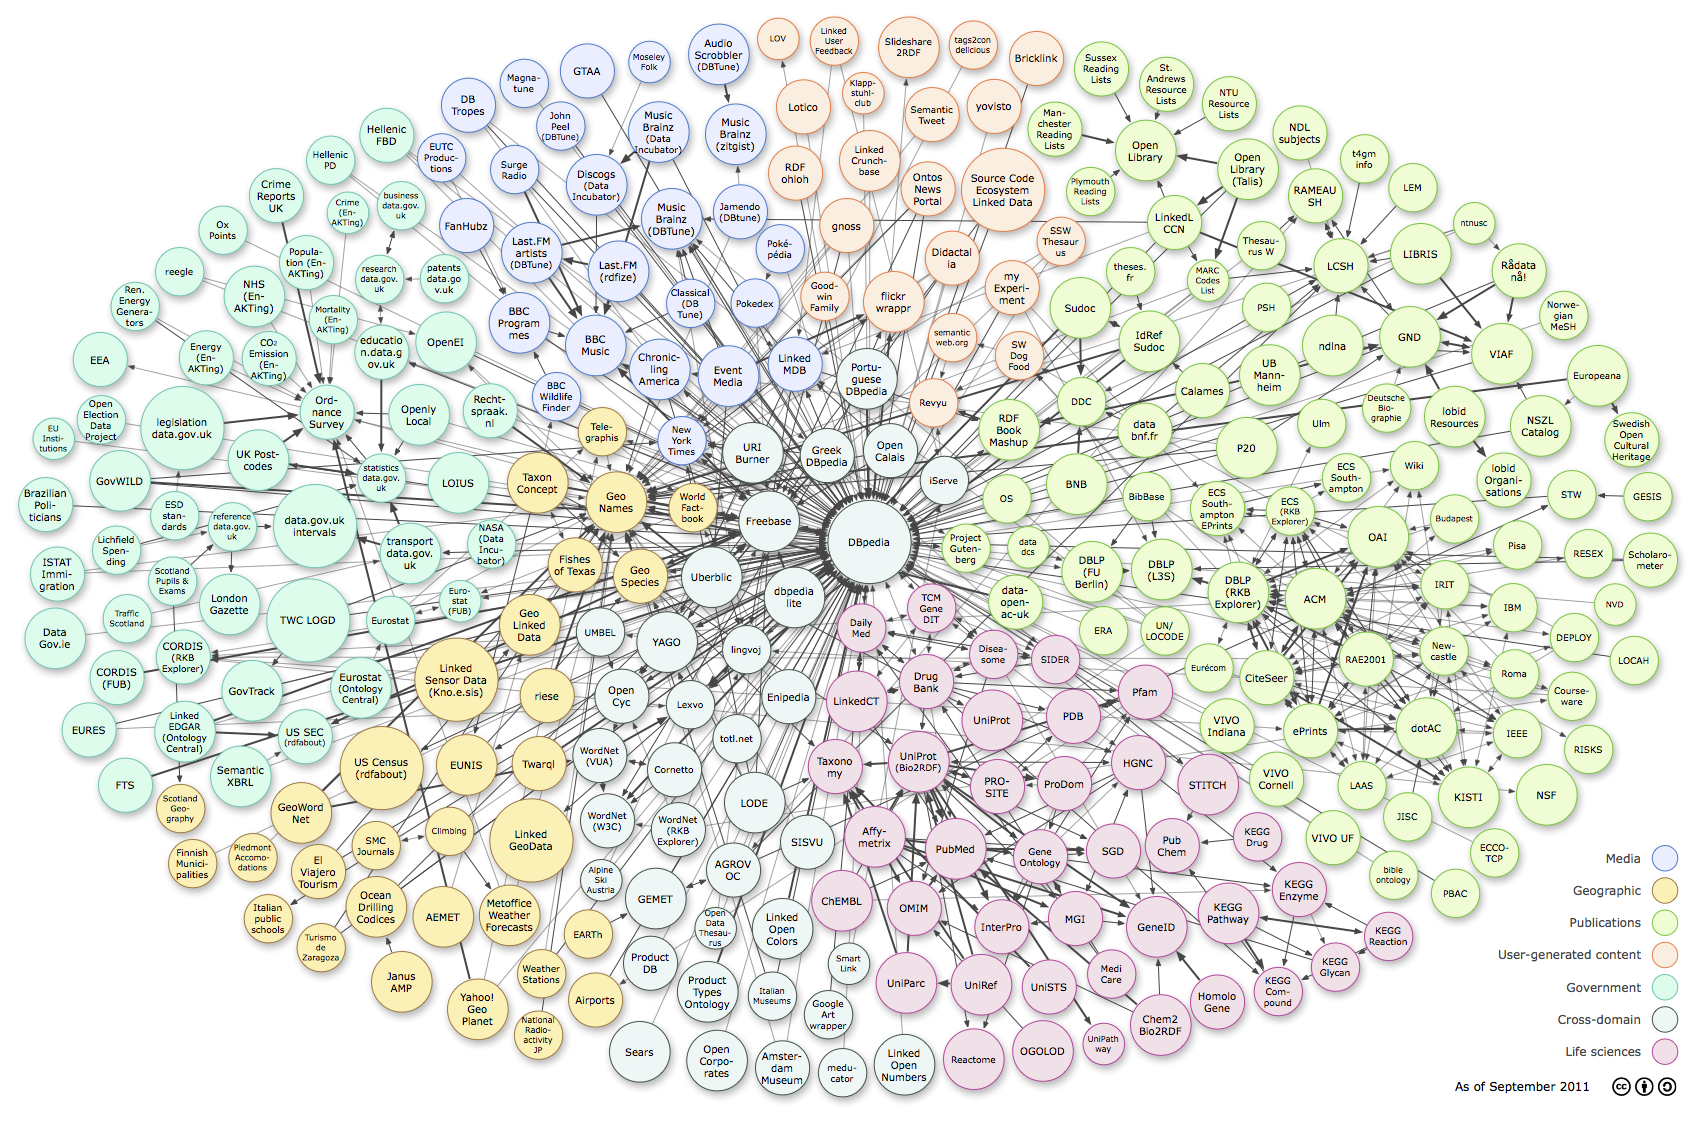
\includegraphics[width=\textwidth]{images/lod-cloud-2011.png}
            \caption{Situazione attuale}
            \label{fig:lod-cloud-2011}
    \end{subfigure}
    \caption{Evoluzione dei dataset pubblicati in LOD (fonte: \protect\url{http://lod-cloud.net})}
    \label{fig:lod-cloud}
\end{figure}

All'intrinseca difficoltà tecnologica propria di qualsiasi conversione di un dataset da un formato ad un altro, si aggiunge la difficoltà della mancata neutralità culturale dei dati che comporta quindi la necessità di effettuare delle precise scelte riguardo il modello descrittivo dei dati (ovvero i metadati che li descrivono) e riguardo il modello concettuale degli stessi, ovvero le ontologie scelte per la conversione.

Quest'ultima scelta diventa ancora più critica in rapporto alla quantità ed eterogeneità degli standard esistenti e attualmente adottati dalle principali entità che si occupano della preservazione dei dati culturali \cite{6}; la mappatura delle ontologie nel dominio LOD (e.g. \cite{7}) è perciò un argomento che sta particolarmente a cuore non solo da un punto di vista tecnico ma anche e soprattutto da un punto di vista concettuale: progetti come \emph{Europeana}\footnote{\url{http://www.europeana.eu}} ne fanno un centrale argomento di discussione.

\newpage
\subsubsection{L'approccio concettuale}

\begin{wrapfigure}{r}{0.4\textwidth}
  \vspace{-20pt}
  \begin{center}
    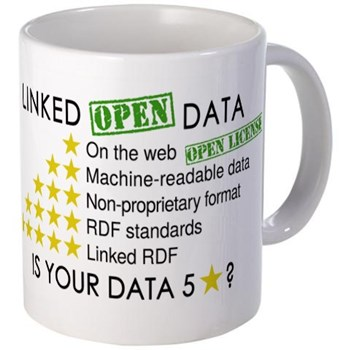
\includegraphics[width=0.4\textwidth]{images/5_star_linked_open_data_mug.jpg}
  \end{center}
  \vspace{-20pt}
  \caption{I vostri LOD sono a 5 stelle? \cite{4}}
  \vspace{-10pt}
\end{wrapfigure}

Prima di pensare all'indispensabile automazione, dal momento che convertire manualmente gli enormi database attualmente in essere sarebbe umanamente impossibile, è necessaria una chiara comprensione di ciò che attualmente esiste per potersene avvantaggiare in maniera proficua.

Tornando alla concettualizzazione di Berners-Lee vista poc'anzi \cite{4}, l'autore aggiunge (nel 2010) un sistema a 5 stelle per definire la qualità dei LOD:
\begin{description}
\item[1 stella] I dati sono sul web in un qualsiasi formato ma \emph{con licenza aperta}.
\item[2 stelle] Come sopra e in più leggibili da una macchina (e.g. una tabella Excel al posto di una scansione della stessa tabella)
\item[3 stelle] Come sopra ma in formato non proprietario (e.g. CSV invece che Excel)
\item[4 stelle] Come sopra ma usano standard del W3C (RDF e SPARQL) per identificare le risorse così da permetterne il collegamento da parte degli utenti
\item[5 stelle] Come sopra e inoltre sono collegati a dati di altre entità.
\end{description}

Questa classificazione si scontra naturalmente con la realtà di fatto: molte istituzioni non sono ancora pronte per il sistema di Berners-Lee perché i dati sono collegati ma non aperti o perché i dataset sono aperti ma debolmente collegati \cite{5}.

Diventa quindi fondamentale la formulazione di un approccio che tenga conto degli sviluppi futuri, attraverso precise metodologie del web semantico e strumenti adeguati, per trarre vantaggio il più possibile dalla ricchezza degli archivi stessi: la formulazione di un processo di conversione è di importanza vitale per garantire la persistenza del dettaglio dei dati di partenza e l'aderenza dei dati di arrivo a degli standard che garantiscano un più che buon livello di interoperabilità. I due approcci possibili in un tale progetto di conversione sono diametralmente opposti.

Il primo mira ad esportare l'intero dataset considerando ogni record come entità ontologica unica e atomica, ottenendo quindi una rappresentazione diretta e appiattita dell'archivio dati. Questa metodologia consente di ottenere velocemente un risultato consistente con la base dati, inscatolando la complessità e l'eventuale divergenza con gli standard all'interno di un'entità che viene gestita come elemento unitario. Collassare gli strati di informazione è pure rischioso per il successivo recupero e riuso dei singoli elementi contenuti nel record, come evidenziato da \cite{8}.

Il secondo prevede un'analisi più complessa e profonda che porti alla divisione di ogni record in elementi atomici intercorrelati riportati su uno strato di astrazione; in questo modo si ottiene un grafo concettuale riusabile e aderente al sistema a 5 stelle di Berners-Lee, al costo di un maggior dispendio di energie nel lavoro di analisi, conversione e revisione dei dati.

\section{Un caso concreto: Zeri e LODE}
Come modello concreto per la conversione di un archivio in LOD è stato considerato l'archivio fotografico della Fondazione Zeri, un'estesa collezione di fotografie di dipinti catalogate in un RDBMS tradizionale con l'obiettivo di esportarle nel dominio LOD adottando CIDOC-CRM come modello descrittivo e concettuale.

Il progetto è stato battezzato \emph{Zeri e LODE}\footnote{da LODE - Live OWL Documentation Environment, \url{http://www.essepuntato.it/lode}}.

\subsection{L'archivio fotografico Zeri}
La collezione fotografica lasciata da Federico Zeri (1921-1998) all'Università di Bologna è un corpus di 290.000 immagini di opere d'arte e monumenti dettagliatamente catalogate e organizzate dal ricercatore lungo tutta la sua carriera\footnote{\url{http://www.fondazionezeri.unibo.it/home/fototeca/00000045_la_fototeca.html}}.\\
La rarità del materiale e della documentazione raccolta nella collezione ne fa un'importantissima fonte di informazione, al punto da venir definita come

\begin{quote}
The first, and no doubt the most important database on art history.\hspace*{\fill}(The Art Tribune, 16 agosto 2010)
\end{quote}

L'archivio è, infatti, prezioso non solo per la rarità e qualità del materiale contenuto, ma soprattutto per il meticoloso lavoro di descrizione storica eseguito da Zeri, che credeva nella fotografia come strumento fondamentale per lo studio e l'analisi filologica delle opere d'arte. Il potere descrittivo e analitico della fotografia in bianco e nero applicato ad un occhio sensibile permetteva di notare sottili variazioni di colore e trama delle opere, paradossalmente meno evidenti in fotografie a colori.

Zeri ha sempre lavorato in modo da costituire un archivio che potesse essere aperto e reso fruibile a chiunque per ricerche, studi e sviluppi; proseguendo gli sforzi del ricercatore, la Fondazione Federico Zeri si è impegnata fin dalla sua costituzione (2002) per rendere accessibile l'archivio fotografico a ricercatori e studenti attraverso la digitalizzazione e catalogazione dell'intera collezione.

\subsection{Il database e la scheda F}
Il risultato del lavoro della Fondazione è un database pubblicamente accessibile in \url{http://www.fondazionezeri.unibo.it} che al momento conta circa 160.000 delle 290.000 fotografie della collezione, consultato da più di 70.000 utenti unici nel solo 2013.

Per ottenenere tale risultato il lavoro di catalogazione è stato preceduto da un'intensa fase analitica: la destinazione d'uso di un simile catalogo richiedeva l'utilizzo di una struttura compatibile con gli standard catalografici italiani definiti dal Ministero per i Beni Culturali\footnote{\url{http://www.iccd.beniculturali.it}} che pure fosse sufficientemente articolata per mantenere la specificità della collezione come organizzata da Federico Zeri.

\begin{figure}[p!]
    \centering
    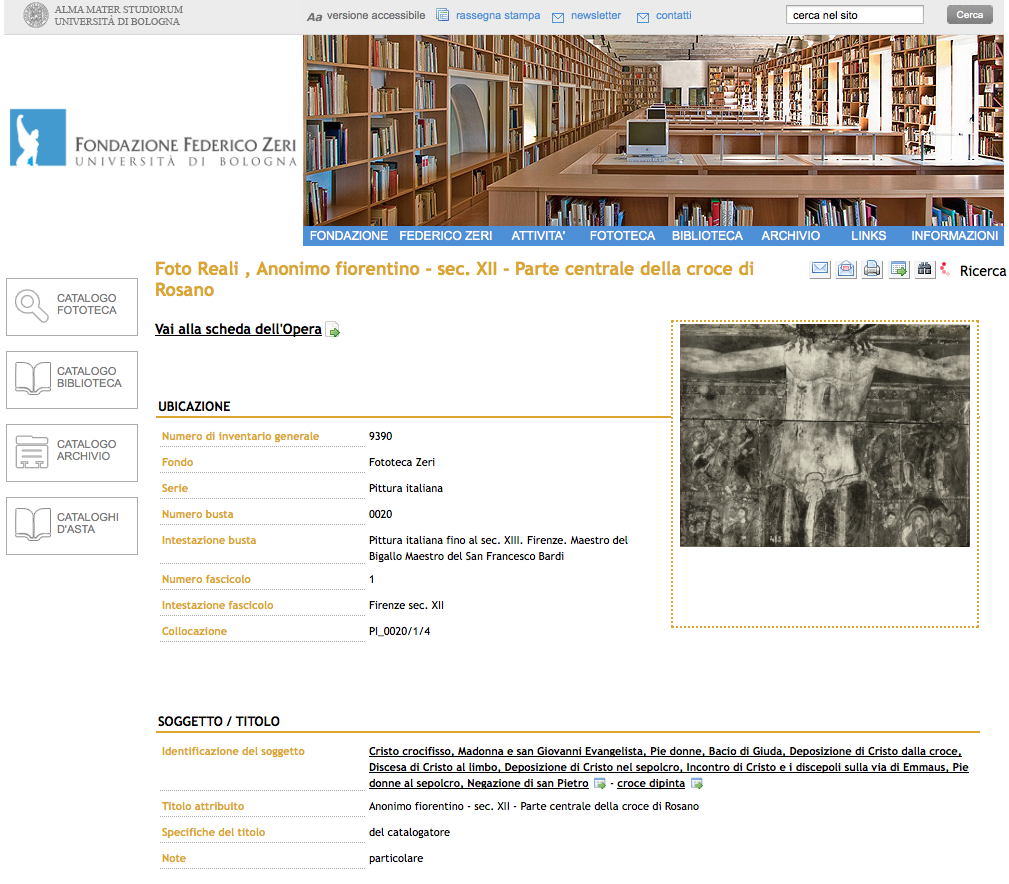
\includegraphics[width=\textwidth]{images/fondazionezeri-screen.png}
	\caption{Esempio di scheda F (fonte: \protect\url{http://www.fondazionezeri.unibo.it/catalogo/})}
	\label{fig:fondazionezeri-screen}
\end{figure}

La scelta del modello descrittivo e concettuale da seguire è ricaduta in modo naturale sulla \emph{Scheda F}\footnote{\url{http://www.iccd.beniculturali.it/index.php?it/387/beni-fotografici}} (dove \emph{F} sta per \emph{Fotografia}) proposto dall'Istituto Centrale per il Catalogo e la Documentazione (ICCD) nella sua versione 3.0.\\
Lo standard \emph{Scheda F} fu accettato solo nel 1999 dopo un intenso dibattito concluso con il riconoscimento, sancito dal ``Testo Unico delle disposizioni legislative in materia di Beni Culturali e Ambientali'' (\cite{16}), della fotografia come bene culturale disciplinato (art 2, comma 2), innalzandola in dignità dal ruolo di pura funzione documentaria che le era stato fino a quel momento attribuito.\\
Nonostante l'iniziale difficoltà di accettazione di questo nuovo standard, causate principalmente dal dettaglio dei campi e la complessità delle norme catalografiche, la validità scientifica della Scheda F è riconosciuta e innegabile, portando nel 2004 ad una revisione (v. 3.00) e attualmente ad una sperimentazione più approfondita con la possibilità di descrivere set complessi oltre a elementi individuali (v. 4.00).\\
Tra i database disponibili sul Web che adottano la Scheda F si possono evidenziare il \emph{SIRPAC - Sistema Informativo Regionale del Patrimonio Culturale del Friuli-Venezia Giulia}\footnote{\url{http://www.sirpac-fvg.org/}}, il portale \emph{Lombardia Beni Culturali}\footnote{\url{http://www.lombardiabeniculturali.it/fotografie/}}, il catalogo \emph{Guarini Patrimonio Culturale}\footnote{\url{http://www.regione.piemonte.it/cultura/GPCWeb/zf/}}, il portale \emph{Beni Culturali Veneto}\footnote{\url{http://catalogo.regione.veneto.it/beniculturali/}}, \emph{L'album di Roma: Fotografie private del Novecento}\footnote{\url{http://www.albumdiroma.it/sicap/opac.aspx?Web=ROMA}}; tali database si avvantaggiano del sistema SIGECweb\footnote{\url{http://www.iccd.beniculturali.it/index.php?it/118/sistema-informativo-generale-del-catalogo-sigec}} attualmente in sviluppo da parte dell'ICCD e in futuro consultabile online.

La complessità e il dettaglio della Scheda F sono allo stesso tempo il maggior punto di forza e di debolezza del modello: le strette norme di catalogazione ne hanno in qualche modo scoraggiato l'adozione per lungo tempo, pure i principi sui quali si basa sono attuali e proiettati verso il riconoscimento degli archivi fotografici come bene con dignità autonoma e non più come documentazione delle opere d'arte fotografate.

Diverse istituzioni si stanno muovendo in questa direzione (e.g. la Berenson Library\footnote{\url{http://itatti.harvard.edu/berenson-library/collections/fototeca-photograph-archive}}, parte della Harvard University, alcuni archivi tedeschi (Hertziana, Kunst Historisches Institute of Florence) parte del Bildarchiv Photo Marburg\footnote{\url{http://www.fotomarburg.de/}}); pure l'attuale interesse all'oggetto fotografico in alcuni casi non è garanzia di precisione nella catalogazione dell'oggetto reale (come avviene, ad esempio, in \emph{Europeana} \cite{8}).

Questo avviene proprio a causa del fisiologico grado di personalizzazione degli standard applicato dalle singole istituzioni per accomodare la specificità dell'archivio catalografico pregresso, spesso sfruttando un ridotto sottoinsieme dei campi messi a disposizione e creando campi fuori standard per conservare dati che altrimenti andrebbero perduti.

Tornando in particolare all'archivio di Zeri, la quantità e particolarità di informazioni registrate sul retro o a margine delle fotografie dallo studioso ha reso necessaria un'espansione e adattamento del modello in essere: degli oltre 300 campi presenti nella versione estesa, la Fondazione Zeri ne ha adottati 113 organizzati in blocchi (definiti \emph{paragrafi}) e aggiungendone alcuni specifici, in parte adottati nello sviluppo della versione 4.0 del modello ministeriale.

I paragrafi replicano l'organizzazione dei dati sulla carta: autore della fotografia, soggetto, titolo, indicazioni cronologiche riguardo lo scatto, movimenti e acquisizioni, dati tecnici, stato di conservazione, copyright e codici identificativi.

Data la natura del soggetto ritratto (opera d'arte) la catalogazione non poteva prescindere dalla raccolta e conservazione delle informazioni a riguardo; è stato quindi affiancato un secondo modello per la descrizione delle opere ritratte, nella fattispecie la \emph{Scheda OA}\footnote{\url{http://www.iccd.beniculturali.it/index.php?it/253/beni-storici-e-artistici}} (dove \emph{OA} sta per \emph{Opera d'Arte}) di ICCD. Qui viene descritto il contenuto semantico della fotografia attraverso altri 79 campi che offrono una dettagliata descrizione riguardo tipo, soggetto, attribuzioni, cronologia, movimenti, materiali, tecniche e riferimenti bibliografici.

Tali informazioni sono principalmente dedotte dalle annotazioni di Zeri sul retro delle fotografie, dalla documentazione che le accompagna e dai volumi presenti nella sua biblioteca.

Ogni Scheda OA è collegata all'insieme delle schede F che ritraggono l'opera; queste ultime sono a loro volta collegate alle relative rappresentazioni digitali (alta e bassa risoluzione, miniatura e scansione del retro della fotografia).

La presenza di due modelli distinti e paralleli permette di fatto la creazione di due cataloghi distinti e correlati, l'uno di materiale fotografico e l'altro di opere d'arte, rendendo quindi possibile una ricerca e navigazione trasversale da parte degli utenti.

I due cataloghi si avvantaggiano di sei \emph{Authority File} (ovvero cataloghi che mirano ad unificare i riferimenti ad entità esterne quali autori, soggetti, bibliografie, etc\ldots\footnote{\url{http://en.wikipedia.org/wiki/Authority_control}}) che forniscono dataset particolareggiati riguardo fotografi, collezioni, artisti, bibliografie, cataloghi d'asta e documenti associati, alcuni di questi accessibili online come database autonomi.

L'indice attuale include, oltre alle fotografie, documenti e cataloghi d'asta, tutti nello stesso contesto; ogni elemento è catalogato e collegato alla scheda dell'opera dal quale deriva, facendo di quest'ultima di fatto il nucleo centrale attorno al quale si dipana tutta la ricerca di Federico Zeri: fotografie, libri e documenti cartacei.

\subsection{Verso un nuovo modello: CIDOC-CRM}\label{sec:towards-a-new-model}
Al momento attuale il database dell'archivio Zeri arriva già a 3 stelle nel sistema di Berners-Lee: è infatti sul web\footnote{\url{http://www.fondazionezeri.unibo.it/catalogo}} con licenza aperta, in formato automatizzabile (\emph{XML}) e standard (\emph{ICCD - Scheda F}). Tali caratteristiche hanno permesso alla Fondazione Zeri di contribuire in maniera significativa a progetti internazionali e portali quali \emph{Europeana}\footnote{\url{http://europeana.eu/}} e \emph{Artstor}\footnote{\url{http://www.artstor.org/}}.

Con l'accrescimento del corpus catalografico e delle esigenze di consultazione e di interscambio con altri cataloghi nasce l'esigenza di esportare i dati in modo più strutturato e in linea con gli standard dei LOD, similarmente a quanto già fatto da altre istituzioni (e.g. \cite{5,9,10,11,12}), il cui lavoro si concentra principalmente sulla conversione del database, la creazione del triple store, il collegamento nel dominio LOD e la realizzazione dell'interfaccia di navigazione.

Nel gennaio del 2013, durante un meeting di due giorni a New York dedicato alle prospettive future per gli archivi della documentazione storico-artistica, è nato il gruppo \emph{International Digital Photo Archive Consortium} (IDPAC), del quale fanno parte, oltre alla Fondazione Federico Zeri, altre tredici istituzioni\footnote{\url{http://www.frick.org/photoarchive/discoveries/future_photoarchives\#sthash.pIMY0SfV.dpuf}} con un archivio totale di 31 milioni di foto di opere d'arte.

Uno degli scopi del gruppo è discutere e verificare la possibilià di creare una piattaforma comune per la condivisione delle rispettive risorse digitali e di collegare i dati per facilitarne l'accesso, in modo da realizzare una vera e popria banca dati globale per la ricerca storica d'arte.

Seppure ancora in fase di esplorazione, il gruppo ha identificato CIDOC-CRM \cite{13} come ontologia più adatta e adattabile a mappare i dati provenienti da molteplici fonti disgiunte, per la sua focalizzazione nel rappresentare la maggior parte degli standard dell'eredità culturale.

Forte di tali esperienze già in essere, il metodo di mappatura è stato focalizzato proprio attorno a CIDOC-CRM, che effettivamente rappresenta la tecnologia più utilizzata nel campo dell'eredità culturale\footnote{\url{http://www.cidoc-crm.org/uses_applications.html}} e permette una concettualizzazione semantica del materiale fotografico in un'ottica FRBR, già ampiamente in uso sebbene talvolta non nel modo adeguato, data la sua natura di dominio bibliografico promosso solo in un secondo momento a framework concettuale.

Inoltre è innegabile l'apporto di altri modelli di produzione di LOD per l'eredità culturale, quali la Library of Congress\footnote{\url{http://id.loc.gov}}, VIAF\footnote{\url{http://viaf.org/}}, CulturaItalia\footnote{\url{http://dati.culturaitalia.it/}}, Bibliothèque nationale de France\footnote{\url{http://data.bnf.fr}}, Deutsche National Bibliothek\footnote{\url{http://www.dnb.de/EN/lds}}, Archives HUB\footnote{\url{http://datahub.io/dataset/archiveshub-linkeddata}}.\\
Tesauri come il \emph{Getty Art \& Architecture Thesaurus®}\footnote{\url{http://www.getty.edu/research/tools/vocabularies/aat/}} e \emph{Iconclass}\footnote{\url{http://www.iconclass.nl/}} sono altresì importanti fonti di dati; anche il \emph{Nuovo Soggettario della Biblioteca Nazionale Centrale Firenze}\footnote{\url{http://thes.bncf.firenze.sbn.it/thes-dati.htm}} offre l'intero tesauro in formato SKOS/RDF, purtuttavia non essendo ancora in LOD.

Considerando infine il modello EDM (\cite{11}) e le linee guida di mappatura di Europeana\footnote{\url{http://www.iconclass.nl/about-iconclass/what-is-iconclass}}, all'interno del quale il catalogo Zeri è già contenuto, lo sforzo è stato quello di definire un modello proprio per il particolare caso dell'archivio, focalizzandosi sulla separazione semantica secondo FRBR e sfruttando altre ontologie (PROV-O\footnote{\url{http://www.w3.org/TR/prov-o/}} e FaBiO\footnote{\url{http://purl.org/spar/fabio}}) non ancora conosciute nel dominio dell'eredità culturale.

\subsection{CIDOC-CRM e FRBR}

\subsubsection{CIDOC Conceptual Reference Model}
Il CIDOC Conceptual Reference Model (CRM)\footnote{\url{http://cidoc-crm.org}} è un modello nato per offrire una struttura formale a supporto della descrizione in concetti e relazioni utilizzati nel campo dell'eredità culturale. Il framework è pensato per essere sufficientemente generico per essere utilizzato in tutta una serie di ambiti culturali quali musei, biblioteche, archivi, etc\dots ovvero per permettere la mappatura di qualsiasi informazione riguardante l'eredità culturale, in modo da risultare una sorta di ``colla semantica'' tra diverse sorgenti di dati con formati diversi.

CIDOC-CRM è il punto d'arrivo di un lavoro di oltre 10 anni fatto dai gruppi \emph{CIDOC Documentation Standards Working Group} e \emph{CIDOC CRM SIG}, accettato come standard ISO (21127:2006\footnote{\url{http://www.iso.org/iso/catalogue_detail?csnumber=34424}}) dal dicembre del 2006.

\subsubsection{Functional Requirements for Bibliographic Records}

La sigla \emph{FRBR} sta per \emph{Functional Requirements for Bibliographic Records} e indica uno schema concettuale disegnato dall'emph{International Federation of Library Associations} (IFLA\footnote{\url{http://www.ifla.org}} nato in ambito bibliografico per la rappresentazione e la classificazione delle informazioni secondo una struttura a livelli \cite{19}.

Attraverso FRBR la catalogazione ``scompone'' il record bibliografico in quattro livelli fondamentali (fig.~\ref{fig:frbf-levels}:
\begin{description}
\item[Work] l'opera di ingegno concettualmente intesa (e.g. \emph{Alice's Adventures in Wonderland} di Lewis Carroll)
\item[Expression] l'espressione, ovvero la realizzazione concettuale di tale opera (e.g. la traduzione italiana \emph{Le avventure di Alice nel Paese delle Meraviglie})
\item[Manifestation] la realizzazione materiale di una Expression (e.g. l'audiolibro \emph{Alice nel Paese delle Meraviglie})
\item[Item] il singolo esemplare di una Manifestation (e.g. la copia del CD \emph{di Fabio} che contiene l'audiolibro \emph{Alice nel Paese delle Meraviglie})
\end{description}

\begin{figure}
  \centering
  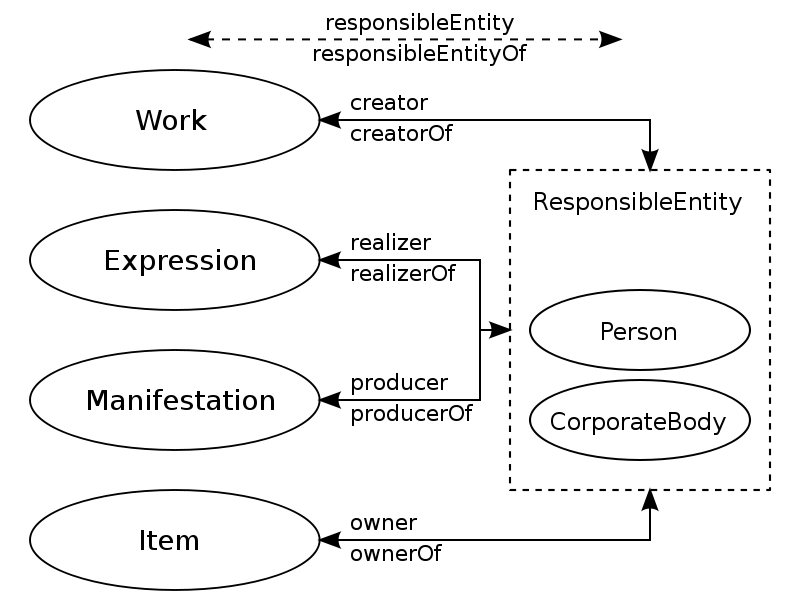
\includegraphics[width=\textwidth]{images/FRBR-Group-2-entities-and-relations.png}
  \caption{I quattro livelli di FRBR e le relazioni con le entità del gruppo 2}\label{fig:frbf-levels}
\end{figure}

Tale suddivisione permette di identificare con precisione il record e unificare i collegamenti in modo concettualmente logico: ad esempio, l'autore viene legato al livello \emph{Work}, l'editore al livello \emph{Manifestation}, il traduttore al livello \emph{Expression} e il possessore al livello \emph{Item} (tali tipologie di entità sono identificate come ``entità del gruppo 2'').

\subsubsection{FRBRoo}

Il naturale punto d'incontro per CIDOC-CRM e FRBR è \emph{FRBRoo}\footnote{\url{http://cidoc-crm.org/frbr_inro.html}}, un'ontologia nata sul modello di CIDOC-CRM per rappresentare la struttura di FRBR in modo che i due modelli possano essere sfruttati insieme.

La prima bozza di FRBRoo è stata pubblicata nel 2006 come modello logicamente rigido che interpreta le concettualizzazioni e le relazioni espresse da FRBR come estensione di CIDOC-CRM.

FRBRoo è arrivato alla sua versione 0.9 nel gennaio del 2008 e approvato dall'IFLA FRBR Review Group nell'agosto del 2008.

\clearpage{\pagestyle{empty}\cleardoublepage}

\chapter{Il progetto Zeri e LODE}

Come già detto in precedenza, il progetto \emph{Zeri e LODE} prevede la conversione dell'archivio della Fondazione Federico Zeri, attualmente implementato sfruttando \emph{MySQL} come RDBMS, in un corpus di triple RDF da caricare in triple store in vista dell'apertura verso la cloud LOD.

Il worflow completo di sviluppo del progetto si articola in quattro punti fondamentali (fig. \ref{fig:zerielode-steps}):
\begin{enumerate}
\item la mappatura del modello della Scheda F in CIDOC-CRM
\item la creazione del triple store
\item l'aggiunta dei collegamenti alla LOD cloud
\item la creazione dell'interfaccia di browsing
\end{enumerate}

In questa sede verranno prese in esame in particolare l'analisi e la realizzazione dei primi due punti.
\begin{figure}
    \centering
    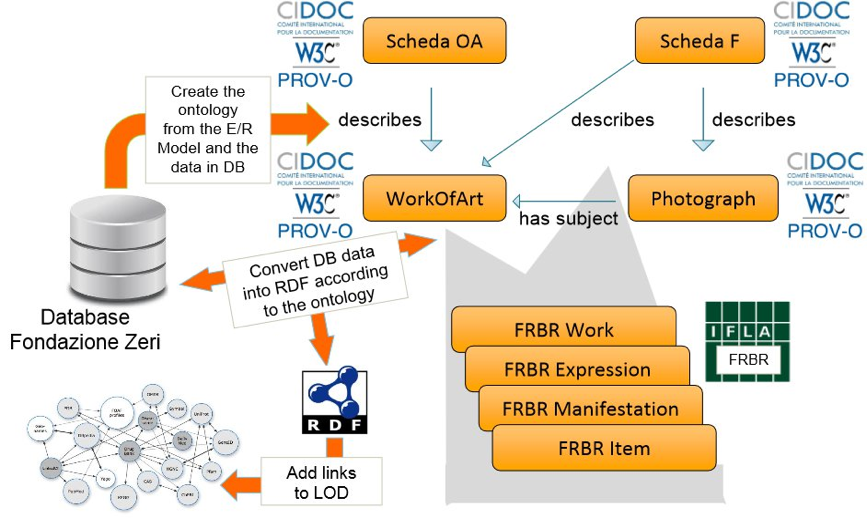
\includegraphics[width=100mm]{images/zeri-steps.png}
	\caption{Workflow di sviluppo}
	\label{fig:zerielode-steps}
\end{figure}

\section{Modello preliminare}

Per le finalità del progetto il formato ideale per l'esportazione dei dati dall'attuale archivio è stato identificato come XML (per ragioni che verranno dettagliate in~\ref{sec:data-analysis}).


\begin{figure}
    \centering
    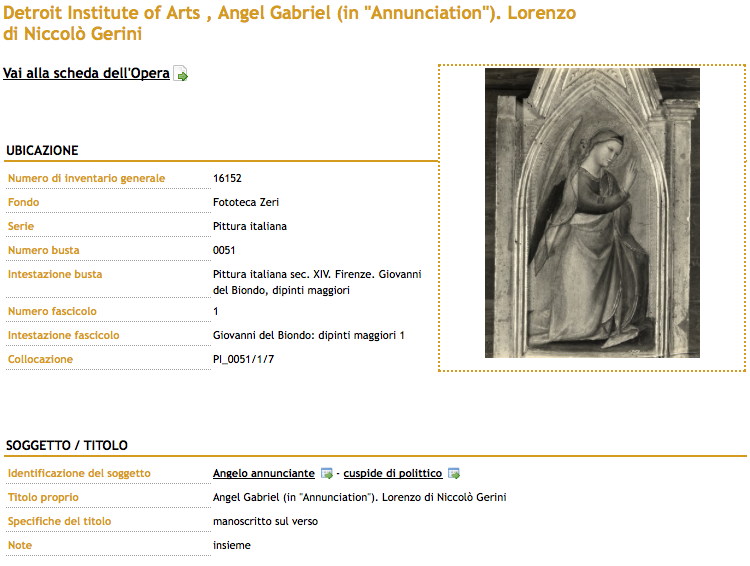
\includegraphics[width=\textwidth]{images/angelo-annunziante.png}
	\caption{Vista parziale di una scheda dell'archivio Zeri online (\protect\url{http://fe.fondazionezeri.unibo.it/catalogo/scheda.jsp?tipo_scheda=F&id=10155})}\label{fig:angelo-annunziante}
\end{figure}

\begin{noindent}
\begin{minipage}{\linewidth}
\begin{lstlisting}[caption=Esempio ideale di conversione, label=listing:conversion-example]
entryf:10155 a fentry:FEntry , crm:E31_Document ;
	crm:P1_is_identified_by "10155" ;
	crm:P70_documents photo:10155 ;
	crm:P102_has_title "Detroit Institute of Arts , Angel Gabriel (in \"Annunciation\"). Lorenzo di Niccolò Gerini." .

photo:10155 a fentry:Photograph , crm:E22_Man-Made_Object ;
	P87_is_identified_by "16152" ;
	P54_has_current_permanent_location [
		a crm:E53_Place ;
		crm:P87_is_identified_by "Giovanni del Biondo: dipinti maggiori 1" ;
		crm:P59i_is_located_on_or_within [
			a crm:E53_Place ;
			crm:P87_is_identified_by "Pittura italiana sec. XIV. Firenze. Giovanni del Biondo, dipinti maggiori" ;
			crm:P59i_is_located_on_or_within [
				a crm:E53_Place ;
				crm:P87_is_identified_by "Pittura italiana" ;
				crm:P59i_is_located_on_or_within [
					a crm:E53_Place ;
					crm:P87_is_identified_by "Fototeca Zeri" .
				] .
			] .
		] .
	] , "PI_0051/1/7" ;
	crm:P62_depicts [
		a crm:E1_CRM_Entity ;
		crm:P1_is_identified_by "Angelo annunciante - cuspide di polittico" ;
		crm:P102_has_title [
			a crm:E35_Title ;
			rdfs:label "Angel Gabriel (in \"Annunciation\"). Lorenzo di Niccolò Gerini" ;
			crm:P3_has_note "manoscritto sul verso" .
		] ;
		crm:P3_has_note "insieme" .
	] .
\end{lstlisting}
\end{minipage}
\end{noindent}

L'obiettivo finale è ottenere una conversione completa della scheda in un insieme di triple RDF. Tale conversione è stata concettualizzata, appunto, sfruttando come base le ontologie CIDOC-CRM e FRBRoo, considerando tuttavia la possibilità (e la necessità) di estenderle nel caso si fossero rivelate troppo limitate o limitanti.

Prendendo come esempio la vista parziale in fig.~\ref{fig:angelo-annunziante}, una traccia di conversione desiderata è riportata nel listato~\ref{listing:conversion-example} (un esempio completo della mappatura di un singolo record a progetto ultimato è riportata nel listato~\ref{listing:sample-output} assieme al record di partenza in XML).

Le domande informali alle quali la concettualizzazione della \emph{Scheda F} tenta di rispondere sono:
\begin{enumerate}
\item Cosa sono le Schede F e le fotografie descritte?
\item Quali sono i soggetti di tali fotografie?
\item Quali sono le entità responsabili nella descrizione degli oggetti e qual è il loro ruolo?
\item Quali sono le fotografie che rappresentano dettagli di un'opera?
\item Quali sono le fotografie in possesso di una data entità in uno specifico intervallo di tempo (e.g. la Fondazione Federico Zeri o la collezione privata dalla quale sono state acquisite)?
\item Quando sono stati creati gli oggetti e da chi?
\item Qual è la collocazione fisica delle fotografie, i.e. quali fotografie sono contenute in una specifica busta (e.g. busta 0014) e in quale fascicolo sono contenute e come sono organizzate le buste all'interno dei fascicoli?
\end{enumerate}

Durante l'analisi e lo sviluppo del progetto si è resa necessaria, per l'appunto, la creazione di un'ontologia ad hoc per poter rappresentare in modo preciso e senza perdita di specificità le varie entità coinvolte all'interno di una singola scheda. Tale ontologia è stata battezzata \emph{F Entry Ontology} (dettagliata in~\ref{sec:feo}) e sfrutta in maniera significativa altre ontologie della suite \emph{SPAR - Semantic Publishing and Referencing}\footnote{\url{http://purl.org/spar/}}.

\section{Requisiti}
Dal punto di vista tecnico la mappatura della \emph{Scheda F} doveva tener conto di diversi aspetti progettuali per poter essere un punto di riferimento, come si pone, per ulteriori sviluppi e riusi anche da parte di altre istituzioni.

Tali aspetti sono:
\begin{description}
\item[automazione] la mappatura dev'essere \emph{automatizzabile}, ovvero strutturata in modo da poter essere elaborata da una macchina quanto più possibile senza l'intervento manuale dell'uomo
\item[scalabilità] la dimensione del catalogo in input è sconosciuta, pertanto la tecnologia di conversione dev'essere pensata per sopportare cataloghi arbitrariamente grandi e pronta a scalare di conseguenza
\item[modularità] per assicurare una miglior semplicità e velocità di sviluppi futuri, la tecnologia dev'essere modulare il più possibile
\item[versatilità] offrendosi come esempio e punto di partenza per archivi diversi con diverse nature dei dati, la mappatura e la tecnologia di conversione devono essere pensate sufficientemente generiche da permettere un rapido adattamento, pur senza sacrificare la peculiarità dell'implementazione per l'archivio Zeri
\end{description}

Tali requisiti sono stati tenuti in considerazione sia nella fase di analisi e conseguente mappatura dei campi della \emph{Scheda F}, sia nel conseguente sviluppo e implementazione a livello di codice (cap.~\ref{chap:implementation})
\clearpage{\pagestyle{empty}\cleardoublepage}

\chapter{Mappatura}\label{chap:mapping}

\section{Il modello per RDF}

L'analisi preliminare ha inizialmente considerato lo specifico sottoinsieme di 113 campi utilizzati dalla Fondazione Zeri, assieme ai campi specifici aggiunti da quest'ultima.\\
Il modello della Scheda F è incredibilmente dettagliato e ricco di informazioni ma ``piatto'': manca perciò di flessibilità nel realizzare collegamenti tra le diverse entità, richiedendo riferimenti ad Authority File o vocabolari controllati per diversi campi e risultando particolarmente vulnerabile a errori ortografici e di inserimento.

Dal momento che l'obiettivo era quello di portare l'archivio fotografico Zeri nel dominio LOD, viste anche le precedenti esperienze (vedi \ref{sec:towards-a-new-model}), CIDOC-CRM è stato scelto come miglior standard in modo da aumentarne al massimo la fruibilità.

L'effettiva mappatura è stata necessariamente sottoposta ad alcuni compromessi, data la natura estremamente flessibile di CIDOC-CRM: lo standard è infatti pensato per coprire una gran varietà di casi, dai musei alle biblioteche, e manca quindi di alcune specificità tipiche di un modello qual è la Scheda F, che essendo disegnato per la fotografia arrichisce in maniera peculiare.

Lo sforzo è stato comunque quello di estendere il meno possibile CIDOC-CRM così da rimanere aderenti allo standard quanto più si è riusciti.

Dal momento che l'obiettivo era rendere disponibile i dati della Scheda F in un triple store, quindi RDF, il linguaggio che è risultato ovvio utilizzare è OWL 2 DL (\cite{8}). Tutto il materiale utilizzato per lo sviluppo della F Entry Ontology (FEO) (secondo la metodologia \emph{SAMOD - Simplified Agile Methodology for Ontology Development\footnote{\url{http://www.essepuntato.it/samod}}}) è già disponibile online\footnote{\url{http://www.essepuntato.it/2014/03/fentry/samod}}, così come la versione attuale dell'ontologia \emph{F Entry Ontology}\footnote{\url{http://www.essepuntato.it/2014/03/fentry}}.

\subsection{L'ontologia F Entry Ontology}\label{sec:feo}
La versione attuale di FEO introduce le classi e le proprietà che caratterizzano i tre concetti fondamentali: la fotografia, l'opera d'arte che ne è soggetto e la stessa Scheda F che descrive la fotografia e il suo soggetto.

La Scheda F è un documento che contiene metadati che descrivono una fotografia che ha per soggetto un'opera d'arte fisica (o un suo particolare) o un gruppo di opere d'arte. Sebbene nella collezione sia presente una sola copia per ogni Scheda F, esistono per la stessa fotografia diverse versioni, e per la stessa opera d'arte sono possibili più fotografie; inoltre la stessa opera d'arte può essere stata sottoposta a trasformazioni ritratte nel tempo da diverse fotografie.

Per registrare correttamente tale complessità di relazioni e caratterizzazioni dipendenti da tempo e contesto dell'entità, la Scheda F, la fotografia e l'opera d'arte sono state descritte e categorizzate concettualmente secondo i termini di Functional Requirements for Bibliographic Recors (FRBR), come segue:
\begin{description}
\item[La Scheda F] contiene dati riguardo la stessa catalogazione, quelli riguardanti la rappresentazione ricadono nel livello \emph{Work} di FRBR e quelli riguardo la sua collocazione ricadono nel livello \emph{Item}.
\item[La fotografia] registra uno specifico evento fotografico in uno specifico momento ma può essere presente in diverse forme nella collezione (e.g. positivo/negativo, diversi tipi di stampa, etc\ldots) e per ogni forma possono esistere copie multiple, ognuna con la propria storia; per questo l'essenza della fotografia è rappresentata dal livello \emph{Work} di FRBR, ogni forma di questa fotografia diventa \emph{Manifestation} e ogni copia individuale ricade nel livello \emph{Item}.
\item[L'opera d'arte] è un oggetto fisico potenzialmente sottoposto a diversi eventi di trasformazione (deterioramenti, restauri, etc\ldots); perciò l'essenza dell'opera d'arte è rappresentata dal livello \emph{Work} di FRBR, il risultato di ogni traformazione dal livello \emph{Manifestation} e le sue caratteristiche fisiche dal livello \emph{Item}.
\end{description}

Tali caratterizzazioni sono soggette ad attribuzione autoriale come risultato di un'attività di produzione che coinvolge degli agenti in uno specifico momento nel tempo.\\
Per modellare questi aspetti sono state importate alcune ontologie preesistenti:
\begin{description}\label{sec:imported-ontologies}
\item[FaBiO - FRBR-aligned Bibliographic Ontology] \cite{6} è un'ontologia basata su FRBR originariamente sviluppata per registrare descrizioni di entità bibliografiche pubblicate o potenzialmente pubblicabili, oppure entità che sono collegate da riferimenti bibliografici, o ancora entità utilizzate per definire questi ultimi. Le entità in FaBiO sono principalmente pubblicazioni testuali quali libri, riviste, giornali e elementi di contenuto quali articoli, relazioni di conferenza e editoriali; oltre a questi descrivono anche blog, pagine web, dataset, algoritmi, immagini, metadati di documenti, protocolli sperimentali, specifiche formali e vocabolari, pezze legali, governative, report tecnici e commeciali e pubblicazioni simili e infine antologie, cataloghi e altre collezioni.
\item[PROV-O - Provenance Ontology] \cite{18} offre un set di classi, proprietà e limiti utilizzabili per rappresentare le informazioni di provenienza riguardo le attività (e.g. la creazione di una fotografia), gli agenti coinvolti (e.g. l'autore della fotografia, il venditore e il compratore in una transazione) e le entità che produce (e.g. il dipinto, la Scheda F, la fotografia).
\end{description}

La versione attuale di FEO è stata strutturata in base alle necessità di descrivere concettualmente e fisicamente la scheda, l'oggetto fotografico e l'oggetto fotografato; una panoramica delle principali classi e relazioni dell'ontologia è visibile in fig.~\ref{fig:feo-mainclasses}.

\begin{figure}
    \centering
    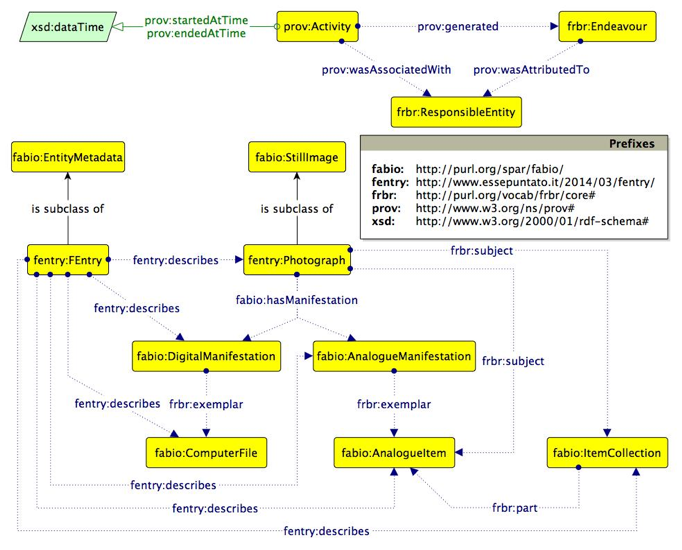
\includegraphics[width=100mm]{images/feo-mainclasses.png}
	\caption{Le relazioni e classi principali definite in FEO - diagramma Graffoo (\protect\url{http://www.essepuntato.it/graffoo})}
	\label{fig:feo-mainclasses}
\end{figure}

Il modello di FEO usa diverse entità descritte in ontologie esterne, principalmente \emph{PROV-O} \cite{22} (prefisso \emph{prov}), la versione OWL 2 DL di FRBR\footnote{\url{http://purl.org/spar/frbr}} (prefisso \emph{frbr}) e \emph{FaBiO} \cite{6} (prefisso \emph{fabio}).

Uno dei concetti principali dell'ontologia è la Scheda F, definita come un particolare documento contenente metadati circa una fotografia e l'oggetto reale rappresentato da quest'ultima. Viene descritta in termini di Work FRBR (i.e. la classe \emph{fentry:FEntry} sottoclasse di \emph{fabio:EntityMetadata}) e di Item FRBR (come file digitale disponibile online, i.e. la classe \emph{fabio:ComputerFile}). La proprietà \emph{fentry:describes} collega istanze di \emph{fentry:FEntry} alle istanze di tutte le altre classi (a prescindere dal livello FRBR), tra le quali \emph{fentry:Photograph}, \emph{fabio:ArtisticWork}, etc\ldots

La fotografia è definita come rappresentazione visuale e statica di un dato oggetto reale (o parte di esso, o di un gruppo di oggetti reali); è descritta come Work FRBR (i.e. la classe \emph{fentry:Photograph} sottoclasse di \emph{fabio:StillImage}), Manifestation FRBR (i.e. le classi \emph{fabio:DigitalManifestation} e \emph{fabio:AnalogueManifestation}) e Item FRBR (i.e. le classi \emph{fabio:ComputerFile} e \emph{fabio:AnalogueItem}). La proprietà \emph{frbr:subject} collega la fotografia all'oggetto reale rappresentato.

L'oggetto reale rappresentato da una fotografia è descritto in termini di Work FRBR (i.e. la classe \emph{fabio:ArtisticWork}), Manifestation FRBR (i.e. la classe \emph{fabio:AnalogueManifestation}) e Item FRBR (la classe \emph{fabio:AnalogueItem}).

\section{La mappatura}
Nel modello della Scheda F è evidente come la divisione in paragrafi la sezioni in parti semanticamente indipendenti e afferenti ad uno specifico concetto FRBR (Work, Expression, Manifestation, Item); ciò permette di procedere alla mappatura affrontando i paragrafi come blocchi unitari, sezioni logiche che coinvolgono un numero limitato di entità legate ai dati documentati nei campi del modello stesso.

In fase di definizione è stato fatto tesoro di tutte le esperienze finora descritte assieme ad alcune più specifiche (e.g. \cite{12}).

La mappatura completa realizzata è visibile in tab. \ref{tab:schedaf-to-owl}; di seguito sono riassunte le principali classi utilizzate per rappresentare le singole entità. Sono tralasciati i livelli FRBR visti in \ref{sec:feo}, concentrandosi invece sulla mappatura in classi CIDOC-CRM (prefisso \emph{crm}).

\subsection{Oggetto fotografico e Scheda F}
Il modella della Scheda F riguarda la descrizione delle fotografie le quali sono, dal punto di vista di CIDOC-CRM, oggetti fisici creati dall'uomo, quindi la classe designata per la rappresentazione è naturalmente \emph{crm:E22 Man-Made Object}. La stessa Scheda F è rappresentata dalla classe \emph{crm:E31 Document} legata alla fotografia dalla proprietà \emph{crm:P70 documents}.

Dal momento che le fotografie dell'archivio Zeri hanno tutte come soggeto una certa opera d'arte, la Scheda F è legata alla relativa Scheda OA, anch'essa istanza di \emph{crm:E31 Document}, tramite la proprietà \emph{crm:P67 refers to}.

\subsection{Livello Work}

L'opera d'arte risulta essere, in CIDOC-CRM, un oggetto fisico creato dall'uomo e pertanto descritto (come la fotografia) tramite la classe \emph{E22 Man-Made Object} e legata alla fotografia dalla proprietà \emph{P62 is depicted by}.

L'autore della fotografia può essere un individuo (e.g. Federico Zeri) o un ente (e.g. Magnum Photo Agency), pertanto per la rappresentazione non è possibile nella gerarchia di classi di CIDOC-CRM oltre alla classe \emph{E39 Actor}, legato alla fotografia dall'attività e dal ruolo caratteristico che ha avuto: e.g. l'autore principale è collegato tramite la proprietù \emph{crm:P14 performed} all'attività di produzione descritta come istanza di \emph{E12 Production}, quest'ultima a sua volta legata alla fotografia dalla proprietà \emph{crm:P108 has produced}; autori alternativi e produttori sono legati in maniera simile con l'aggiunta, nel caso sia presente, del ruolo avuto nella produzione della fotografia, descritto con la classe \emph{pro:roleInTime} fornita dalla Publishing Roles Ontology - PRO\footnote{\url{http://purl.org/spar/pro}}.

\subsection{Livello Manifestation}

Dal punto di vista di FRBR la descrizione dell'oggetto ricade nel livello Manifestation; qui vengono documentate alcune caratteristiche specifiche dell'oggetto stesso, quali:
\begin{description}
\item[Materiali] dei quali è composto l'oggetto, descritte con la classe \emph{crm:E57 Material} e collegate con la proprietà \emph{crm:P45 consist of}.
\item[Dimensioni] ovvero altezza, larghezza, spessore, diametro: sebbene nella Scheda F siano sezionate in campi ad hoc, CIDOC-CRM non dispone di tale specificità, offrendo una generica classe \emph{crm:E54 Dimension} ulteriormente dettagliata con le proprietà \emph{crm:P2 has type}, \emph{crm:P90 has value} e \emph{crm:P91 has unit}; le dimensioni così istanziate vengono poi legate all'oggetto dalla proprietà \emph{crm:P43 has dimension}\footnote{e.g. photo (E22) \emph{has dimension (P43)} height of photo (E54) \emph{has type (P2)} height (E62), \emph{has unit (P91)} mm (E58), \emph{has value (P90)} 227 (E60)}.
\item[Tecnica] usata nella produzione della fotografia, è rappresentata come istanza di \emph{crm:E55 Type} collegata a \emph{crm:E12 Production} tramite la proprietà \emph{crm:P32 used technique}; l'istanza di \emph{crm:E12 Production} è a sua volta collegata alla fotografia tramite la proprietà \emph{crm:P108 was produced by}. Nel particolare caso delle tecniche e più in generale tutte le volte in cui viene utilizzata come classe descrittiva \emph{crm:E55 Type}, la scelta del tipo è mappata in vocabolari controllati da ICCD o analoghi tesauri.
\end{description}

Oltre ai dati riguardanti l'oggetto fisico, il modello della Scheda F permette al catalogatore di aggiungere alla creazione della foto delle informazioni cronologiche e spaziali sul luogo dello scatto. Dal momento che tale creazione riguarda comunque l'oggetto, ricade anch'essa nel livello Manifestation. Le classi scelte per rappresentare gli eventi di creazione e produzione sono \emph{crm:E65 Creation} e \emph{crm:E12 Production} legati all'oggetto rispettivamente dalle proprietà \emph{crm:P94 was created by} e \emph{crm:P108 was produced by} e a loro volta legate ad una istanza di \emph{crm:E53 Place} tramite la proprietà \emph{crm:P7 took place at} per le indicazioni spaziali e ad un'istanza di \emph{crm:P4 Period} tramite \emph{crm:P10 falls within} per le indicazioni cronologiche.

Altri dati d'interesse riguardanti il livello Manifestation sono il tipo dell'oggetto (e.g. positivo, negativo, stampa, etc\dots) naturalmente rappresentato da un'istanza di \emph{E55 Type} che mappa il vocabolario controllato di ICCD e legato all'oggetto tramite \emph{crm:P2 has type}; il numero di oggetti fisici che compongono l'oggetto stesso, rappresentati da un'istanza di \emph{crm:E60 Number} legata con \emph{crm:P57 has number of parts}.

Le possibili relazioni con altri oggetti fotografici (de-composizione per fotografie complesse o correlate) sono descritte nel modello della Scheda F con l'indicazione della raccolta superiore e sono pertanto state rappresentate come collegamento via \emph{crm:P46 forms part of} all'istanza specifica di \emph{E18 Physical Thing}.

Infine, anche le indicazioni di copyright ricadono nel livello Manifestation e sono state descritte con la classe \emph{crm:E30 Right} legata all'oggetto fotografico tramite la proprietà \emph{crm:P104 is subject to}\footnote{il dominio della proprietà \emph{P104} è la classe \emph{crm:E72 Legal Object}, il collegamento è tuttavia legittimo grazie al fatto che la classe \emph{crm:E22 Man-Made Object} deriva sia da \emph{crm:E71 Man-Made Thing} che da \emph{crm:E72 Legal Object}}.

\subsection{Livello Item}

Il modello della Scheda F include alcuni campi per documentare la posizione attuale (geografica e archivistica) dell'oggetto fotografico ed eventuali posizioni precedenti. In CIDOC-CRM tali posizioni sono descritte tramite la classe \emph{crm:E53 Place}, anche quelle archivistiche (e.g. inventario e collocazione). Per definire la posizione attuale dell'oggetto è stata scelta la proprietà \emph{crm:P54 has current permanent location} mentre per le precedenti posizioni la proprietà è \emph{crm:P53 has former or current location}.

Nel definire le coordinate temporali di queste ultime è stata sfruttata la \emph{Time Ontology in OWL}\footnote{\url{http://www.w3.org/TR/owl-time/}} che offre delle primitive particolari (i.e. \emph{time:Istant}, \emph{time:hasBeginning} e \emph{time:hasEnd}) per specificare ulteriormente la blanda precisione della classe \emph{crm:E52 Time-Span} di CIDOC-CRM. Tali coordinate temporali sono state applicate (con \emph{crm:P4 has time-span}) ad un'istanza di \emph{crm:E9 Move} legata a sua volta all'oggetto fotografico tramite la proprietà \emph{crm:P25 moved}.

Eventuali posizioni annidate (e.g. la collocazione all'interno di un edificio posizionato geograficamente oppure la busta all'interno di un fascicolo) sono state collegate tra di loro tramite la proprietà \emph{crm:P89 falls within}.

Le condizioni fisiche e lo stato di conservazione riguardano altresì il livello Item. Tali informazioni sono state descritte con la classe \emph{crm:E3 Condition State} e legate all'oggetto con la proprietà \emph{crm:P44 has condition}. Dal momento che lo stato di conservazione è definito in un vocabolario controllato, le varie tipologie sono state mappate in istanze di \emph{crm:E55 Type} e legate alla condizione tramite \emph{crm:P2 has type}.

\subsection{Proprietà della Scheda F}

Le proprietà della Scheda F stessa consistono principalmente di dati amministrativi, il più importante dei quali è l'identificatore interno al catalogo, descritto con la classe \emph{crm:E42 Identifier} tramite la proprietà \emph{crm:P48 has preferred identifier}.

Il tipo di scheda identifica il modello all'interno di quelli forniti da ICCD, nel caso specifico è dunque sempre uguale a ``F'' ed è descritto tramite \emph{crm:E55 Type} e relativa proprietà \emph{crm:P2 has type}.

L'istituto o ente responsabile della conservazione, non potendo fare assunzioni specifiche sulla sua natura, è descritto come istanza di \emph{crm:E40 Legal Body} e legato alla scheda tramite la proprietà \emph{crm:P50 has current keeper}.

Ulteriori dati vengono registrati per:
\begin{itemize}
\item il catalogatore che ha creato la prima versione della scheda, istanza di \emph{crm:E39 Actor}, legato all'istanza di \emph{crm:E65 Creation} tramite \emph{crm:P14 carried out by} e quest'ultima a sua volta legata all'oggetto scheda da \emph{crm:P94 created}; le coordinate temporali sulla catalogazione sono descritte tramite la classe \emph{crm:E52 Time-Span} e legate all'attività di creazione con \emph{crm:P4 has time-span}.
\item gli aggiornamenti effettuati sulla catalogazione, analoghi alla catalogazione ma descritti tramite un'istanza di \emph{crm:E81 Trasformation} in luogo di \emph{crm:E65 Creation}.
\end{itemize}

\clearpage{\pagestyle{empty}\cleardoublepage}

\chapter{Implementazione tecnica}\label{chap:implementation}

Per l'effettiva conversione del tracciato della Scheda F in uso dalla Fondazione Zeri era necessaria un'applicazione che si occupasse di realizzare in maniera automatica la mappatura definita in \ref{tab:schedaf-to-owl} richiedendo scarsa o nulla interazione da parte dell'utente; è stato quindi sviluppato uno strumento in \emph{Python} in grado di ritornare in output uno o più file RDF a fronte di un dataset in XML come input.\\

Il codice aggiornato è disponibile su \emph{GitHub} all'indirizzo \url{https://github.com/ciromattia/zerielode} ed è rilasciato con licenza MIT\footnote{\url{http://opensource.org/licenses/MIT}}.

\section{Analisi dei dati}\label{sec:data-analysis}

Per l'analisi dei dati di partenza si è partiti dal dump completo dell'archivio Zeri in formato XML (del quale è riportato un esempio nel listato \ref{listing:sample-fzeri}).

\lstinputlisting[language=XML, caption=Esempio di record Zeri, label=listing:sample-fzeri]{images/sample_fzeri.xml}

\label{sec:fakerecord}Lo script \texttt{schema\_builder.py} è stato usato per generare un record fasullo che contenesse tutti i campi effettivamente in uso nell'intero dataset, in modo da avere una istantanea della situazione reale: il risultato si può leggere nel listato~\ref{listing:fzeri-fakerecord}. La necessità di generare tale report è nata dall'impossibilità di affidarsi all'analisi del singolo record, in quanto non necessariamente completo di tutti i campi, alcuni dei quali per giunta mutualmente esclusivi.

Il record generato contiene ovviamente informazioni incoerenti tra di loro ma fondamentali per la revisione della struttura e la scrittura dell'algoritmo di parsing del dataset (cfr. tab.~\ref{tab:schedaf-to-owl} e figg.~\ref{fig:mapping-v3-1} e seguenti). Ha inoltre fornito degli importanti indizi sul formato del contenuto dei campi stessi, semplificando il successivo lavoro di conversione in statement RDF.

L'organizzazione del singolo record è in paragrafi distinti; l'albero della singola scheda raggiunge una profondità di 3 o 4 nodi a seconda della ripetibilità del campo.

Il primo livello è il \texttt{PARAGRAFO} che divide la scheda in aree concettuali; ogni paragrafo contiene una serie di campi singoli, opzionalmente racchiusi dal livello medio \texttt{RIPETIZIONE} nel caso il paragrafo stesso sia ripetibile più di una volta all'interno della stessa scheda (e.g. \emph{possessore} o \emph{collocazioni precedenti}).

L'elenco completo dei campi e della loro struttura è stato dettagliato in tracciati (tab.~\ref{tab:fzeri-schedaF} e successive) incrociati con le specifiche fornite da ICCD (\cite{14,15})

L'analisi si è quindi concentrata sulla mappatura di tale struttura appiattita verso una completa riconversione dei dati in un insieme di \emph{statement} RDF coerenti con FEO. Per realizzare l'effettiva conversione è stato realizzato un sistema di script che prenda in input l'esportazione in formato XML del database attuale dell'archivio fotografico Zeri e produca uno o più file RDF da caricare in seguito in un triple store.

\section{Scelta del linguaggio e delle tecnologie}

Inizialmente, data la natura di formato dei dati in input (XML) si è pensato alla definizione di un foglio di stile (XSL) applicando il quale si sarebbe ottenuta la trasformazione del dataset in un insieme di statement RDF. L'impegno nel definire tale foglio di stile è risultato però gravoso e non espandibile a meno di ulteriori sforzi: l'eventuale foglio di stile sarebbe infatti stato limitato in diversi modi (si noti che tali limitazioni non sono assolute ed esiste la possibilità di implementazione, il costo di sviluppo per superare i limiti presentati risulta però decisamente svantaggioso):
\begin{description}
\item[struttura] Un foglio di stile è legato ad una sola e precisa struttura dei dati in input: nel caso di dati mal strutturati o definiti la trasformazione XSLT è prona ad errori e fallimenti più di un approccio programmatico.
\item[formato] Il foglio di stile produce uno e un solo formato in output: questo può risultare limitante dal momento che RDF può essere espresso in svariati linguaggi (Turtle, N3, RDF/XML, \ldots).
\item[flessibilità] La possibilità di suddividere l'output in molteplici file è di difficile implementazione, soprattutto all'interno di un singolo foglio di stile.
\end{description}

XSL è stato quindi abbandonato preferendo in sua vece la flessibilità e comodità di \emph{Python} e dell'ottimo modulo \emph{rdflib}, che ha consentito l'implementazione completa e robusta della mappatura concettuale a livello applicativo.

Lo sviluppo si è svolto attorno ad uno script principale che funge da entry point della procedura di conversione, disegnato per accettare diversi argomenti che ne modificano il comportamento in particolar modo per quanto riguarda l'output generato.

\begin{noindent}
\begin{minipage}{\linewidth}
\begin{lstlisting}[frame=single,caption=Help in linea di \texttt{fzeri\_schedaF\_to\_owl.py}, label=listing:usage]
usage: fzeri_schedaF_to_owl.py [-h] [--single-entry] [-o OUTPUT_FILE]
                               [-f FORMAT]
                               source_file [source_file ...]

FZeri to CIDOC-CRM catalog conversion script.

positional arguments:
  source_file           FZeri catalog file(s) path

optional arguments:
  -h, --help            show this help message and exit
  --single-entry        Outputs entries in a single file for each one.
  -o OUTPUT_FILE, --output OUTPUT_FILE
                        Output file or directory name
  -f FORMAT, --format FORMAT
                        Output format (xml|n3|turtle|nt|pretty-xml|trix)
\end{lstlisting}
\end{minipage}
\end{noindent}

L'esigenza di differenziare il formato in output è nata dalla varietà di strumenti esistenti per il consumo di RDF: ad esempio, il software \emph{Protégé}\footnote{\url{http://protege.stanford.edu}} è risultato incapace di caricare gli statement generati in formato \emph{Turtle}, mentre ha caricato correttamente il formato \emph{RDF/XML}.

Per lo stesso motivo è stato utile aggiungere come opzione la possibilità di avere in output, in luogo di un unico file contenente tutto il grafo RDF, un file singolo per ogni scheda all'interno della directory specificata, così da renderne possibile il caricamento parziale o completo anche su macchine senza un adeguato quantitativo di memoria disponibile.

A fianco dello script principale è stata creata la classe \texttt{FZeriParserSchedaF} definita in \texttt{fzeri\_parser\_schedaF.py} che si occupa di percorrere l'albero di una singola scheda in formato XML e di generare il corrispondente set di statement RDF.

L'attuale mappatura viene eseguita da un set di funzioni specifiche per ogni paragrafo: tale scelta è stata effettuata in virtù della specificità dei singoli paragrafi così da mantenere il più possibile la granularità delle informazioni attualmente registrate nel dataset in input.

\section{Implementazione interna}

\subsection{Panoramica di funzionamento}
Lo script principale carica il file in input in una struttura \texttt{etree} (caricata dal modulo \texttt{lxml} oppure da \texttt{xml.etree.ElementTree} nel caso il primo non sia presente nel sistema) e genera un nuovo grafo RDF tramite la chiamata \texttt{Graph()} di \texttt{rdflib}, associando i namespace delle ontologie utilizzate.

Rileva quindi tutti gli elementi \texttt{SCHEDA} dell'albero XML e per ognuno crea una nuova istanza della classe \texttt{FZeriParserSchedaF} passando come argomento il sottoalbero (ovvero la singola scheda) e il grafo RDF globale\footnote{nel caso sia specificato l'argomento \texttt{--single-entry}, per ogni singola scheda viene creato un nuovo grafo che viene poi salvato su un file individuale.}, chiamando infine il metodo \texttt{parse()} dell'oggetto istanziato.

\texttt{parse()} cicla su tutti i nodi \texttt{PARAGRAFO} estrapolandone l'eventuale ripetibilità e chiamando per ognuno la specifica funzione di mappatura del paragrafo. Tale funzione associa in primis il paragrafo al livello FRBR corrispondente, quindi procede con l'aggiunta degli statement RDF al grafo passato dal chiamante.

\subsection{Ontologie utilizzate}
Per mappare i campi della Scheda F sono state sfruttate, oltre alle ontologie citate in \ref{sec:imported-ontologies}, ulteriori ontologie di appoggio già utilizzate nel campo dell'eredità culturale. Nella fattispecie sono state importate le seguenti ontologie (riportate con il relativo prefisso e namespace):
\begin{description}
\footnotesize
\item[CIDOC-CRM] (crm:) http://www.cidoc-crm.org/cidoc-crm/
\item[Dublin Core] (dc:) http://purl.org/dc/elements/1.1/
\item[DCMI Metadata Terms] (dcterms:) http://purl.org/dc/terms/
\item[F Entry Ontology] (fentry:) http://www.essepuntato.it/2014/03/fentry/
\item[FRBR] (frbr:) http://purl.org/vocab/frbr/core\#
\item[FRBR-aligned Bibliographic Ontology] (fabio:) http://purl.org/spar/fabio/
\item[Friend of a Friend] (foaf:) http://xmlns.com/foaf/0.1/
\item[The PROV Ontology] (prov:) http://www.w3.org/ns/prov\#
\item[Publishing Roles Ontology] (pro:) http://purl.org/spar/pro
\item[Quantities, Units, Dimensions and Types] (qudt:) http://qudt.org/vocab/unit\#
\item[The Time Ontology] (time:) http://www.w3.org/2006/time\#
\end{description}

Oltre ai namespace delle ontologie ne sono stati istanziati altri 15 con base \texttt{http://fe.fondazionezeri.unibo.it/} per indirizzare le singole istanze delle entità create durante il parsing della scheda.

\subsection{Dettaglio procedurale della classe \texttt{FZeriParserSchedaF}}

La classe \texttt{FZeriParserSchedaF} accetta su nuova istanziazione due parametri: l'albero XML della scheda F e il grafo RDF al quale aggiungere gli statement convertiti. L'effettiva conversione viene attuata alla chiamata del metodo \texttt{parse()}.

\subsubsection{parse()}
Il metodo \texttt{parse()} si preoccupa di inizializzare il grafo della singola scheda (con il metodo \texttt{init\_graph()}), quindi cicla su ogni nodo di tipo \texttt{PARAGRAFO}, rilevandone l'eventuale ripetibilità e passandolo come argomento al metodo preposto al parsing di quello specifico nodo, ottenuto prefissando l'attributo \texttt{etichetta} del nodo XML, normalizzato in modo da poter essere un simbolo di funzione legale, con la stringa \texttt{parse\_paragraph\_}:
\begin{Verbatim}[fontsize=\footnotesize]
getattr(self, "parse_paragraph_" + child.attrib["etichetta"].lower().
        replace(' ', '_').replace('(', '').replace(')', ''))(child)
\end{Verbatim}

\subsubsection{init\_graph()}
Il metodo \texttt{init\_graph()} è responsabile di inizializzare la conversione della scheda in statement RDF.

L'assegnazione (e il mantenimento come proprietà della classe) delle proprietà \texttt{self.myentry}, \texttt{self.myphoto} e \texttt{self.production} risultano vitali in quanto tali entità rappresentano gli oggetti principali che verranno poi usati nel parsing dei singoli paragrafi per costruire il grafo di entità e relazioni.

In particolare è qui che l'oggetto ``Scheda F'' viene definito come istanza di \texttt{crm:E31 Document} e di \texttt{fentry:FEntry} e l'oggetto ``Fotografia'' come istanza di \texttt{crm:E22 Man-Made Object} e di \texttt{fentry:Photograph}, rendendo subito evidente il duplice binario sul quale procede l'utilizzo delle ontologie importate. Le due istanze sono legate tra loro tramite le proprietà \texttt{crm:P70 documents} e \texttt{fentry:describes}.

In questo metodo viene anche creata un'istanza di \texttt{crm:E1 CRM Entity} per rappresentare l'\emph{Opera d'arte} rappresentata dalla fotografia: le ragioni di questo sono spiegate nell'analisi del paragrafo \texttt{AUTHOR}.

Nei paragrafi seguenti si farà riferimento agli oggetti ``Scheda F'' e ``Fotografia'' come \texttt{schedaF} e \texttt{photo}.

\begin{quote}
\textbf{Nota:} l'ontologia utilizzata per CIDOC-CRM (\url{http://cidoc-crm.org/rdfs/cidoc_crm_v5.0.4_official_release.rdfs}) non contiene le definizioni per le proprietà inverse (i.e. \texttt{owl:inverseOf}); è perciò stato necessario, per ogni relazione in CIDOC-CRM, aggiungere due statement l'uno inverso dell'altro così da rendere comodo l'eventuale utilizzo di ragionatori automatici.
\end{quote}

Infine, il metodo crea una nuova istanza di \texttt{crm:E12 Production}, legandola a \texttt{myphoto} tramite la proprietà \texttt{crm:P108 produced}. La necessità di creare anticipatamente l'attività di produzione della fotografia è nata dall'analisi dei dati riguardanti l'attività stessa, quasi sempre non riguardanti concretamente la medesima \emph{attività} bensì il medesimo \emph{scopo} (e.g. autorialità, stampa, pubblicazione, \ldots). Non esistendo un modo per indicare questa particolarità in CIDOC-CRM, si è scelto di creare un'unica attività di produzione della fotografia alla quale legare in seguito, attraverso la proprietà \texttt{crm:P9 consists of}, le singole istanze di \texttt{crm:E12 Production} estrapolate dai dati in input.

\subsubsection{parse\_paragraph\_copyright()}
Nel paragrafo \texttt{COPYRIGHT} è mantenuta la data di scadenza di eventuali diritti d'autore. L'informazione è stata riportata come nota allegata ad un'istanza di \texttt{crm:E30 Right} poiché i dati in input non seguono una formattazione standard in grado di essere compresa e convertita automaticamente.

\subsubsection{parse\_paragraph\_notes()}
Il semplice paragrafo \texttt{NOTES}, contenente un solo campo ad inserimento libero, viene naturalmente descritto come \texttt{Literal} legato a \texttt{photo} dalla proprietà \texttt{crm:P3 has note}.

\subsubsection{parse\_paragraph\_supervisor()}
Il paragrafo \texttt{SUPERVISOR} contiene informazioni riguardo il supervisore della catalogazione, ovvero il responsabile del controllo per la correttezza delle informazioni. Pur non essendo dettagliato come altri campi riferiti a persone fisiche, si è scelto di descriverlo con la classe \texttt{crm:E39 Actor}. Il legame con la \texttt{schedaF} avviene in due modi: il primo tramite l'attività \texttt{crm:E65 Creation}, il secondo grazie all'aggiunta della classe \texttt{foaf:Document} a \texttt{schedaF} che permette di utilizzare \texttt{pro:roleInTime} con le due proprietà \texttt{pro:relatesToDocument} e \texttt{pro:holdsRoleInTime}.

\subsubsection{parse\_paragraph\_classification()}
Le informazioni contenute nel paragrafo \texttt{CLASSIFICATION} ricadono quasi in toto nel livello \emph{Manifestation} di \texttt{photo}.

Includono informazioni inventariali quali il numero di inventario, mappato in un'istanza di \texttt{crm:E42 Identifier} e la collocazione, mappata in una serie di \texttt{crm:E53 Place}. Contrariamente a quanto sarebbe istintivo pensare, la classe \texttt{crm:E53 Place} non è limitata ai luoghi fisici ma definisce anche posizioni logiche (e.g. il riferimento all'interno di uno scaffale o il numero progressivo all'interno di una serie), quindi è perfettamente in linea con i dati da rappresentare.

Dal momento che la collocazione può essere espressa in maniera annidata (i.e. busta all'interno di una scatola a sua volta all'interno di un fascicolo), le istanze delle varie collocazioni vengono opportunamente annidate tramite la proprietà \texttt{crm:P59 has section (is located on or within)}.

La posizione più specifica è legata a \texttt{photo} tramite la proprietà \texttt{crm:P54 has current permanent location}, scelta al posto di \texttt{crm:P55 has current location} per evidenziare la natura definitiva della collocazione.

L'unico campo di questo paragrafo che interessa \texttt{schedaF} è l'identificativo che la collega alla relativa \emph{Scheda OA}, espresso con la proprietà \texttt{crm:P67 refers to} all'istanza di \texttt{crm:E31 Document}.

\subsubsection{parse\_paragraph\_ownership()}
Il paragrafo \texttt{OWNERSHIP} contiene i dati riguardanti la proprietà legale attuale di \texttt{photo}. In CIDOC-CRM tuttavia non esiste un'entità che lo esprima, pertanto è necessario descriverlo attraverso l'attività temporale che ha portato al cambio di proprietà (\texttt{crm:E8 Acquisition}) legata a \texttt{photo} con la proprietà \texttt{crm:P24 transferred title of (changed ownership through)}, attività poi legata all'appropriata istanza di \texttt{crm:E39 Actor} via \texttt{crm:P22 transferred title to}.

\subsubsection{parse\_paragraph\_codes()}
Il paragrafo \texttt{CODES} definisce una serie di codici per \texttt{schedaF}: la tipologia di scheda secondo ICCD (quindi sempre uguale al valore ``F'') è legata tramite \texttt{crm:P2 has type}, il numero identificativo e il codice regionale sono rappresentati come istanze di \texttt{crm:E42 Identifier} collegate via \texttt{crm:P48 has preferred identifier}.

L'ente competente per la tutela è descritto da \texttt{crm:E40 Legal Body} e legato da \texttt{crm:P50 is current keeper of}. Per completezza è stata aggiunta anche la classe \texttt{foaf:Agent} con la proprietà \texttt{foaf:name}, mentre \texttt{pro:roleInTime} è stata usata in previsione di potenziali modifiche future dell'ente competente per la tutela.

\subsubsection{parse\_paragraph\_cataloguing()}
Le informazioni riguardo il catalogatore iniziale, i.e. il creatore della scheda, sono registrate nel paragrafo \texttt{CATALOGUING}: è perciò naturale legare \texttt{schedaF} ad un'attività \texttt{crm:E65 Creation} e quest'ultima all'istanza di \texttt{crm:E39 Actor} che rappresenta il catalogatore e all'istanza di \texttt{crm:E52 Time-Span} preposta alla descrizione della data nella quale è avvenuta la catalogazione. In questo caso, essendo una stringa formattata arbitrariamente, si è scelto di rappresentarla come \texttt{crm:E49 Time Appellation} legata al timespan tramite \texttt{crm:P78 is identified by (identifies)}.

\subsubsection{parse\_paragraph\_updating()}
Del tutto analogo al precedente, il paragrafo \texttt{UPDATING} è ripetibile e mantiene in ogni sua ripetizione i dati di tutti i catalogatori che hanno successivamente modificato la scheda. Le entità utilizzate sono le medesime, la sola differenza è nell'attività utilizzata, \texttt{crm:E81 Transformation} in luogo di \texttt{crm:E65 Creation}.
\subsubsection{parse\_paragraph\_object()}
All'interno del paragrafo \texttt{OBJECT} sono registrate le informazioni riguardanti l'oggetto fotografico nella sua Manifestazione (come intesa in FRBR), quindi il soggetto è \texttt{photo}. Per rappresentare tre campi (tipologia e formato) è stato scelto di utilizzare l'ontologia \emph{Dublin Core} al posto di CIDOC-CRM perché ritenuta più immediata e adeguata, nella fattispecie \texttt{dc:type} e \texttt{dc:format}.

Le misure fisiche della fotografia (altezza, larghezza, spessore, diametro) nella \emph{Scheda F} sono specifiche per tipologia di misura; la genericità di CIDOC-CRM mette a disposizione una generica classe \texttt{crm:E54 Dimension}. Tale classe è stata usata per la rappresentazione delle singole misure, il cui tipo è stato quindi specificato con la proprietà \texttt{crm:P2 has type} e il cui valore con \texttt{crm:P90 has value}. Le unità di misura sono legate, in CIDOC-CRM, alla singola dimensione, a differenza di com'è specificato nel modello della Scheda F; pertanto per ogni singola dimensione istanziata ne viene impostata la tipologia con \texttt{crm:P2 has type} e l'unità di misura con \texttt{crm:P91 has unit}. Per rendere quanto più fruibili e standard anche le unità di misura, sono state convertite in modo da sfruttare l'ontologia \emph{QUDT}\footnote{\url{http://qudt.org/vocab/unit/}} attraverso l'hash \texttt{unit\_fzeri\_to\_qudt}.

\subsubsection{parse\_paragraph\_subject()}
Il paragrafo \texttt{SUBJECT} contiene informazioni riguardo il soggetto della fotografia, ovvero l'opera d'arte rappresentata. Non potendo fare assunzioni di alcun genere sulla natura del soggetto stesso, questo è descritto da un'istanza della classe \texttt{crm:E1 CRM Entity}, ovvero la classe più generica in CIDOC-CRM; è poi legato a \texttt{photo} attraverso \texttt{crm:P62 depicts}.

Il dato più vicino ad un identificatore è una stringa, perciò viene legato al soggetto con \texttt{crm:P1 is identified by}; l'eventuale tipologia e nota sono legati come al solito tramite \texttt{crm:P2 has type} e \texttt{crm:P3 has note}.

Un approccio diverso è stato invece adottato per rappresentare i titoli. Il modello della Scheda F predispone infatti tre diversi campi per \emph{titolo proprio}, \emph{titolo parallelo} e \emph{titolo attribuito}. Sebbene CIDOC-CRM metta a disposizione la proprietà \texttt{crm:P102 has title}, la tipologia di titolo sarebbe specificabile solamente con la sottoproprietà \texttt{crm:P102.1 has type}; RDF tuttavia non supporta proprietà di proprietà. Si è scelto quindi di sotto-classare in FEO la proprietà \texttt{crm:P102 has title} in tre diverse proprietà:
\begin{description}
\item[\texttt{fentry:hasProperTitle}] per il titolo proprio, inversa di \texttt{fentry:isProperTitleOf};
\item[\texttt{fentry:hasParallelTitle}] per il titolo parallelo, inversa di \texttt{fentry:isParallelTitleOf};
\item[\texttt{fentry:hasAttributedTitle}] per il titolo attribuito, inversa di \texttt{fentry:isAttributedTitleOf}.
\end{description}

Al titolo è stata aggiunta per apertura agli standard anche la classe \texttt{dcterms:title}.

\subsubsection{parse\_paragraph\_author()}\label{sec:parse-paragraph-author}
Il paragrafo \texttt{AUTHOR}, diversamente da tutti gli altri, si riferisce all'opera ritratta, ovvero all'autore del soggetto. Per questo motivo si è riflettuto a lungo se riportare i dati nel grafo RDF generato. Una volta implementata la mappatura e l'immissione in LOD anche per l'archivio di schede OA, tali dati saranno sicuramente ridondanti e potenzialmente ignorabili; in questo stadio di sviluppo, tuttavia, si è scelto di mantenerli per evitare la possibile perdita di informazione, seppure creando in questo modo un'entità parziale.

L'oggetto \texttt{artwork} (ovvero \emph{Opera d'arte}) è stato descritto con la classe \texttt{crm:E1 CRM Entity} per evitare qualsiasi assunzione sulla sua natura. Il paragrafo \texttt{AUTHOR} è ripetibile e per ogni ripetizione viene creata un'istanza di \texttt{crm:E12 Production} alla quale viene collegata l'istanza di \texttt{crm:E39 Actor} tramite la proprietà \texttt{crm:P14 carried out by}; il nome proprio, pseudonimo e altro nome dell'autore sono descritti con istanze di \texttt{crm:E82 Actor Appellation} legate tramite \texttt{crm:P131 is identified by}.

Il modello della scheda F prevede anche l'eventuale specifica del contesto culturale dell'autore (e.g. \emph{Scuola toscana}): non essendo disponibile una classe in CIDOC-CRM per mantenere questa informazione è stata definita in FEO la classe \texttt{fentry:hasCulturalContext}.

\subsubsection{parse\_paragraph\_dating()}
Le informazioni cronologiche riguardo l'oggetto fotografico sono registrate nel paragrafo \texttt{DATING}.

Tali informazioni, in quanto riferite all'atto della produzione della fotografia, sono state incentrate all'attività \texttt{crm:E12 Production} di \texttt{photo}, dettagliate sfruttando la classe \texttt{crm:E52 Time-Span}. Quest'ultima classe in CIDOC-CRM è debolmente definita, nel senso che permette una grossa varietà di tipologie di input; per mantenere la granularità e non perdere informazioni si è scelto di utilizzare l'ontologia \texttt{Time} e classare il timespan anche come \texttt{time:TemporalEntity}, in modo da poterne definire inizio e fine come \texttt{time:Instant} con proprietà \texttt{time:hasBeginning} e \texttt{time:hasEnd}.

Più in generale questo approccio è stato adottato in tutti gli utilizzi dove \texttt{crm:E52 Time-Span} risultava troppo poco definito per mantenere la qualità dell'informazione in input.

La motivazione e sorgente dell'attribuzione\footnote{e.g. \emph{nota sul retro} o \emph{ricerca storica}} è stata descritta con \texttt{crm:E13 Attribute Assignment} e la proprietà \texttt{crm:P17 was motivated by}.

\subsubsection{parse\_paragraph\_photographer()}
Il paragrafo \texttt{PHOTOGRAPHER} è analogo ad \texttt{AUTHOR} ma si riferisce al creatore dell'oggetto fotografico; è inoltre ripetibile quindi, come già illustrato, per ogni ripetizione è stata creata un'istanza di \texttt{crm:E12 Production} legata in seguito alla \texttt{crm:E12 Production} principale tramite \texttt{crm:P9 consists of (forms part of)}.

L'autore è rappresentato da un'istanza di \texttt{crm:E39 Actor} e legato all'attività via \texttt{crm:P14 performed}; a sua volta è identificato (\texttt{crm:P131 is identified by}) da una istanza \texttt{crm:E82 Actor Appellation} e può opzionalmente avere un indirizzo che è stato descritto tramite la classe \texttt{crm:E51 Contact Point}.

Similarmente a quanto fatto per il paragrafo \texttt{DATING}, le motivazioni e la fonte per l'attribuzione dell'autorialità sono state rese con un'istanza di \texttt{crm:E13 Attribute Assignment} legata tramite \texttt{crm:P17 was motivated by} per quanto riguarda la motivazione e tramite \texttt{crm:P16 used specific object} per la fonte.

Non esistendo in CIDOC-CRM una metodologia specifica per indicare il ruolo all'interno di un'attività senza proprietà di proprietà (non supportate da RDF), il ruolo dell'autore è stato descritto sfruttando l'ontologia PRO, nella fattispecie con la classe \texttt{pro:roleInTime} legata a \texttt{photo} con la proprietà \texttt{pro:relatesToDocument} e all'autore con \texttt{pro:holdsRoleInTime}; il ruolo stesso è stato specificato via \texttt{pro:withRole}.

\subsubsection{parse\_paragraph\_production\_and\_publishing()}
Del tutto analogo a \texttt{PHOTOGRAPHER}, il paragrafo \texttt{PRODUCTION AND PUBLISHING} (ripetibile) viene processato in maniera pressocché identica, affidandosi a PRO per la definizione del ruolo.

In aggiunta ai campi presenti in \texttt{PHOTOGRAPHER}, questo paragrafo può contenere informazioni riguardo il luogo di edizione/stampa, rappresentato da un'istanza di \texttt{crm:E6 Place} legata tramite \texttt{crm:P7 took place at} alla \texttt{crm:E12 Production} relativa, e un'indicazione cronologica, per la quale è stata usata la classe \texttt{crm:E52 Time-Span} definita ulteriormente con \texttt{crm:E49 Time Appellation} (senza quindi l'utilizzo di \emph{Time Ontology}).

\subsubsection{parse\_paragraph\_place\_and\_date\_of\_the\_shot()}
Per la descrizione del paragrafo \texttt{PLACE AND DATE OF THE SHOT} è stata scelta come classe \texttt{crm:E65 Creation} perché ritenuta concettualmente più adatta di \texttt{crm:E12 Production}. Se infatti l'atto fisico dello scatto può essere vista come un'attività di produzione di un oggetto tangibile, l'atto del fotografare è più astratto e pertinente dunque ad una sfera più immateriale.

\texttt{crm:E65 Creation} è legato a \texttt{photo} con la proprietà \texttt{crm:P94 created} e alle coordinate temporali tramite \texttt{crm:P4 has time-span} ad un'istanza di \texttt{crm:E52 Time-Span} ulteriormente definita da \texttt{crm:E49 Time Appellation}.

Per le coordinate spaziali invece è stato scelto di descrivere l'occasione, ovvero l'evento\footnote{e.g. \emph{Asta Christie's 11/07/1980}}, nel quale la fotografia è stata scattata con la classe \texttt{crm:E4 Period}, legata all'attività di creazione dalla proprietà \texttt{crm:P10 falls within (contains)}; i dati riguardanti precise coordinate geografiche quali \emph{nazione} e \emph{città} sono invece state descritte tramite \texttt{crm:E53 Place} e incapsulate nel caso fossero presenti entrambe con la proprietà \texttt{crm:P89 falls within} già vista in precedenza.

\subsubsection{parse\_paragraph\_relations\_with\_other\_photographic\_objects\_negative()}
Il paragrafo \texttt{RELATIONS WITH OTHER PHOTOGRAPHIC OBJECTS (NEGATIVE)} contiene informazioni riguardo l'eventuale negativo/diapositiva/altro (a cui in seguito sarà fatto riferimento come ``negativo'') dal quale è stata realizzata la stampa.

Il negativo è definito come \texttt{crm:E22 Man-Made Object} analogamente alla fotografia, legato a \texttt{photo} attraverso un'istanza di \texttt{crm:E12 Production} cui è collegato via \texttt{crm:P16 used specific object (was used for)}.

Le informazioni registrate per il negativo sono l'identificativo, assegnato via \texttt{crm:P1 is identified by}, la tipologia, descritta in un'istanza di \texttt{crm:E55 Type} che fa riferimento ad un vocabolario controllato di ICCD e legata tramite \texttt{crm:P2 has type}, e la posizione, rappresentata da \texttt{crm:E53 Place} legato al negativo dalla proprietà \texttt{crm:P55 has current location}.

\subsubsection{parse\_paragraph\_digital\_image()}
Nel paragrafo \texttt{DIGITAL IMAGE} sono contenuti i metadati e il percorso per eventuali rappresentazioni digitali dell'oggetto fotografico.

Per ogni ripetizione del paragrafo viene creata un'entità che afferisce alle classi \texttt{crm:E38 Image} e \texttt{fabio:DigitalManifestation}, quest'ultima per permettere l'impostazione della struttura FRBR tramite collegamento a \texttt{schedaF} con \texttt{fentry:describes} e a \texttt{photo} con \texttt{fabio:hasManifestation}; per quanto riguarda CIDOC-CRM invece la relazione è tramite la proprietà \texttt{crm:P138 represents} verso \texttt{photo}.

Il campo con il percorso del file viene utilizzato per la creazione di una seconda entità con classi \texttt{crm:E38 Image} e \texttt{fabio:ComputerFile}, a sua volta legato all'immagine di cui sopra tramite \texttt{frbr:exemplar} e \texttt{crm:P138 represents} e a \texttt{schedaF} con \texttt{fentry:describes}.

\subsubsection{parse\_paragraph\_provenance()}
Il paragrafo ripetibile \texttt{PROVENANCE} documenta tutti i movimenti dell'oggetto fotografico nella storia conosciuta.

Per rappresentare le informazioni di questo paragrafo si sono usati due oggetti principali: un'istanza di \texttt{crm:E53 Place} e un'istanza di \texttt{crm:E9 Move}, la prima legata alla seconda tramite \texttt{crm:P26 moved to (was destination of)} e la seconda legata a \texttt{photo} con \texttt{crm:P25 moved (was moved by)}.

Le coordinate temporali sono legate a \texttt{crm:E9 Move} tramite \texttt{crm:E52 Time-Span}, per definire il quale è stata usata l'ontologia Time analogamente al paragrafo \texttt{DATING} e ottenendo quindi la definizione dell'inizio e della fine della permanenza in un determinato luogo.

Le coordinate spaziali geografiche sono potenzialmente annidate, quindi per ognuna è stata istanziata la classe \texttt{crm:E53 Place} e infine sono state legate opportunamente tra di loro con \texttt{crm:P59 has section (is located on or within)}; la \emph{collezione} è invece stata rappresentata tramite \texttt{crm:E46 Section Definition} e legata al luogo più specifico con la proprietà \texttt{crm:P87 is identified by}.

Il luogo più specifico, infine, è collegato a \texttt{photo} dalla proprietà \texttt{crm:P53 has former or current location}.

\subsubsection{parse\_paragraph\_location()}
La posizione fisica e geografica dell'oggetto fotografico è indicata nel paragrafo \texttt{LOCATION}.

Tale posizione è chiaramente descritta come istanza di \texttt{crm:E53 Place} legato a \texttt{photo} da \texttt{crm:P55 has current location}; anche qui, analogamente ad altri paragrafi, ci sono una serie di specifiche geografie annidate (i.e. regione, provincia, città, archivio) per ognuna delle quali viene istanziata una \texttt{crm:E53 Place}, gestendo in seguito gli annidamenti con la proprietà \texttt{crm:P59 has section (is located on or within)}.

Si è scelto invece di descrivere i dati riguardanti la \emph{collezione} e la \emph{posizione precisa} (sezione) tramite legami \texttt{crm:P87 is identified by} alla \texttt{crm:E53 Place} più specifica.

\subsubsection{parse\_paragraph\_state\_of\_preservation()}
Per le condizioni di conservazione registrate nel paragrafo \texttt{STATE OF PRESERVATION}, CIDOC-CRM offre la classe \texttt{crm:E3 Condition State}, legata a \texttt{photo} da \texttt{crm:P44 has condition}.

La condizione viene definita con una \texttt{rdfs:label} e ne viene registrata la tipologia con un legame \texttt{crm:P2 has type} verso un'istanza di \texttt{crm:E55 Type} scelta in un vocabolario controllato di ICCD.

\subsubsection{parse\_paragraph\_relation\_to\_other\_objects()}
Le eventuali relazioni con altri oggetti espresse nel paragrafo \texttt{RELATION TO OTHER OBJECTS}, non avendo dei precisi riferimenti quali identificativi, collocazioni, etc\ldots sono descritte in CIDOC-CRM come legami da \texttt{photo} a \texttt{crm:E18 Physical Thing} via \texttt{crm:P46 is composed of (forms part of)}.

\clearpage{\pagestyle{empty}\cleardoublepage}

\chapter{Valutazione}

La realizzazione di uno strumento di conversione quanto più automatico possibile ha portato ad una serie di scelte importanti sul trattamento dei dati in input.

La scelta dell'utilizzo di alcune ontologie in luogo di altre, specialmente non ancora conosciute nel dominio dell'eredità culturale, è allo stesso tempo coraggiosa e rischiosa: la mappatura è stata effettuata nell'ottica di mantenere quanto più possibile il dettaglio delle informazioni contenute e pertanto utilizzando classi specifiche di ontologie finora conosciute solamente in campo biblioteconomico (i.e. la suite \emph{SPAR - Semantic Publishing and Referencing}\footnote{\url{http://sempublishing.sourceforge.net}} e \cite{6}). Il rischio è che tali ontologie non vengano accettate come standard nel campo del cultural heritage, costringendo il progetto \emph{Zeri e LODE} a rivederne l'utilizzo oppure ad accettare una parziale fuoriuscita dallo standard.

In questo senso è fondamentale la cooperazione e il dialogo con altri archivi fotografici e progetti che siano diretti all'apertura in LOD della propria base informativa, così da creare una solida base per l'interoperabilità dei dati.

Durante lo sviluppo è poi stato notato come l'iniziale mappatura teorica fatta a fronte dei tracciati riportati in \ref{tab:fzeri-schedaF} e seguenti abbia subito una sostanziale rilettura e parziale modifica con l'analisi dei dati reali XML (cfr.~\ref{sec:fakerecord}) a causa di strutture parzialmente diverse, campi inutilizzati e valori non coerenti con la classe di destinazione definita in prima battuta (cfr. tab.~\ref{tab:schedaf-to-owl} e figg.~\ref{fig:mapping-v3-1} e seguenti).

L'utilizzo di un approccio procedurale quale lo scripting in \emph{Python} ha permesso uno sviluppo più rapido a fronte della scrittura e successiva applicazione di un foglio di stile; la sua divisione in moduli, classi e funzioni indipendenti permette anche un veloce adattamento nel caso il formato di input dovesse essere modificato, grazie anche all'utilizzo della classe \texttt{etree} che permette un rapido accesso all'albero XML e alla presenza di metodi individuali per il parsing dei singoli paragrafi. In questo modo, dovesse l'input variare, sarà sufficiente modificare a livello minimale la parte di lettura dell'albero XML per ottenere la generazione dello stesso output.

L'utilizzo dell'ottima libreria \texttt{rdflib}\footnote{\url{https://rdflib.readthedocs.org/en/latest/}} è risultato importante anche in virtù dei futuri sviluppi: dalla versione 4.0.1 infatti sono state integrate le classi \texttt{SPARQLStore} e \texttt{SPARQLUpdateStore} assieme al kit di funzionalità per il dialogo con un endpoint \emph{SPARQL}: tali funzionalità risulteranno fondamentali in un eventuale futura creazione diretta del triple store in LOD e implementazione di una forma di sincronizzazione bidirezionale con l'archivio Zeri.

Infine, il progetto presentato è stato relazionato nel paper \emph{Converting the Zeri photo archive in Linked Open Data: formalizing the conceptual model} \cite{29} proposto all'\emph{International Conference on Theory and Practice of Digital Libraries (TPDL 2014)}\footnote{\url{http://www.dl2014.org}} e riconosciuto come contributo significativo nel campo della conservazione dell'eredità culturale (accettato tra i 30 \emph{full paper} a fronte di 107 proposte ricevute).

\clearpage{\pagestyle{empty}\cleardoublepage}

\chapter*{Conclusioni}
\rhead[\fancyplain{}{\bfseries
CONCLUSIONI}]{\fancyplain{}{\bfseries\thepage}}
\lhead[\fancyplain{}{\bfseries\thepage}]{\fancyplain{}{\bfseries
CONCLUSIONI}}

\addcontentsline{toc}{chapter}{Conclusioni} 

Il progetto \emph{Zeri e LODE}, pur ponendosi come obiettivo principale la conversione dell'attuale base informativa dell'archivio fotografico della Fondazione Zeri in un dataset RDF e il successivo inserimento nella rete dei LOD, si offre come base metodologica per conversioni di altre collezioni analoghe di materiale fotografico.

L'archivio Zeri è una fra le più importanti collezioni di fotografie di opere d'arte a livello mondiale; la possibilità di analizzare la molteplicità e variabilità delle catalogazioni ivi contenute ha permesso di approfondire lo sviluppo considerando diversi scenari e svariate interpretazioni nella mappatura da un modello ricco e piatto quale quello della Scheda F disegnata dall'Istituto Centrale per il Catalogo e la Documentazione (ICCD) ad un modello articolato e generico quale CIDOC-CRM.

Grazie a questo sono state poste delle solide basi di modellazione grazie alla realizzazione della F Entry Ontology (FEO) che accompagna ed estende lo standard di CIDOC-CRM nei punti ritenuti carenti o troppo generici.

Terminata la fase di sviluppo degli strumenti per la conversione, la naturale prosecuzione del progetto prevede la creazione di un triple store e una prima esportazione dell'archivio convertito in un dataset pubblicamente accessibile; quindi sarà necessario collegare i dati al dominio LOD (e.g. \emph{DBPedia}\footnote{\url{http://dbpedia.org}}, \emph{Europeana}\footnote{\url{http://europeana.eu/}}, \emph{ResearchSpace}\footnote{\url{http://www.researchspace.org}}, \emph{VIAF}\footnote{\url{http://viaf.org}}, etc\ldots\footnote{una lista parziale si trova in \url{http://linkeddata.org/data-sets}}).

Il passo successivo è naturalmente lo sviluppo di un'interfaccia navigabile e ricercabile per la presentazione del dataset contenuto nel triple store, rendendola responsiva e accessibile, basata su interrogazioni incentrate sui facet, come ad esempio il modello di \emph{Virtuoso} usato da \emph{Dbpedia}\footnote{\url{http://dbpedia.org/fct/}}, oppure sfruttando framework quali \emph{Sesame}\footnote{\url{http://www.openrdf.org}}.\\
L'obiettivo principale dovrebbe in ogni caso essere quello di rendere l'interfaccia accessibile e usabile anche e soprattutto da browser Web Semantici\footnote{alcuni riportati in \url{http://wiki.dbpedia.org/OnlineAccess\#h28-13}}.

Un ulteriore sviluppo inoltre potrebbe considerare l'implementazione in FEO dei vocabolari controllati di ICCD utilizzati per la compilazione dei campi della Scheda F, oltre alla realizzazione di un'analoga mappatura e conversione per il modello \emph{Scheda OA} di ICCD, così da avere i due cataloghi paralleli e sfruttare i riferimenti incrociati\footnote{a questo proposito si ricordi di eliminare o uniformare la mappatura delle informazioni sull'autore dell'opera provenienti dal paragrafo \texttt{AUTHOR} della Scheda F - cfr.~\ref{sec:parse-paragraph-author}}.

Le considerazioni sulla mappatura potrebbero essere, infine, ulteriormente estese, anche grazie all'analisi di ulteriori casi di studio: le entità e le proprietà offerte da CIDOC-CRM sono adeguate a descrivere un archivio fotografico con sufficiente particolarità, oppure sussiste la necessità di estendere CIDOC-CRM per non rischiare di perdere informazioni?


\renewcommand{\chaptermark}[1]{\markright{\thechapter \ #1}{}}
\lhead[\fancyplain{}{\bfseries\thepage}]{\fancyplain{}{\bfseries\rightmark}}
\appendix

\chapter{Mappatura}
\rhead[\fancyplain{}{\bfseries \thechapter \:Mappatura}]
{\fancyplain{}{\bfseries\thepage}}

In questa Appendice viene riportata la mappatura effettiva applicata per la conversione del dataset XML da \emph{Scheda F} a \emph{CIDOC-CRM}.\\
Per compattezza sono state omesse le proprietà basilari (e.g. \emph{rdfs:label}) desumibili dal codice.

Per confronto e completezza è stata inclusa anche l'iniziale mappatura teorica, in seguito modificata a fronte delle strutture reali.

\begin{center}
\tiny

\begin{longtable}{ | p{1cm} | p{8cm} | p{3cm} | }
\caption{Mappatura effettiva da Scheda F a CIDOC-CRM} \label{tab:schedaf-to-owl} \\
\hline \multicolumn{1}{|p{1cm}|}{\cellcolor{lightyellow}\textbf{Campo Scheda F}} & \multicolumn{1}{p{8cm}|}{\cellcolor{lightyellow}\textbf{mappatura CIDOC-CRM}} & \multicolumn{1}{p{3cm}|}{\cellcolor{lightyellow}\textbf{Note}}\\ \hline
\endfirsthead
\multicolumn{3}{c}%
{{\bfseries \tablename\ \thetable{} -- continua da pag. precedente}} \\
\hline \multicolumn{1}{|p{1cm}|}{\cellcolor{lightyellow}\textbf{Campo Scheda F}} & \multicolumn{1}{p{8cm}|}{\cellcolor{lightyellow}\textbf{mappatura CIDOC-CRM}} & \multicolumn{1}{p{3cm}|}{\cellcolor{lightyellow}\textbf{Note}} \\ \hline
\endhead
\hline \multicolumn{3}{r}{{continua a pag. successiva}}\\
\endfoot
\hline \hline
\endlastfoot

  \multicolumn{3}{|l|}{\cellcolor{lightcyan}COPYRIGHT}\\ \hline
  CRPD & entry - CRM.P104\_is\_subject\_to - CRM.E30\_Right & \\
  & CRM.P3 has note - Literal & \\ \hline

  \multicolumn{3}{|l|}{\cellcolor{lightcyan}NOTES}\\ \hline
  OSS &  entry - CRM.P3\_has\_note - Literal & \\ \hline

  \multicolumn{3}{|l|}{\cellcolor{lightcyan}SUPERVISOR}\\ \hline
  FUR &  entry - CRM.P94i\_was\_created\_by - CRM.E65\_Creation & \\
   & CRM.P11\_had\_participant - CRM.E39\_Actor & \\ \hline
  
  \multicolumn{3}{|l|}{\cellcolor{lightcyan}CLASSIFICATION}\\ \hline
  SERCDOA &  entry - CRM.P67\_refers\_to - CRM.E31\_Document & \\ \hline
  INVN &  photo - CRM.P149\_is\_identified\_by - CRM.E42\_Identifier & \\ \hline
  \pagebreak
  UBFP &  photo - CRM.P54\_has\_current\_permanent\_location - CRM.E53\_Place & \multirow{12}{3cm}{UBFP, UBFS, UBFT e UBFU sono collocazioni annidate, perciò il CRM.E53\_Place più interno è inscatolato nel più esterno tramite CRM.P59i} \\
   & CRM.P87\_is\_identified\_by - CRM.E44\_Place\_Appellation & \\
   & CRM.P59i\_is\_located\_on\_or\_within - CRM.E53\_Place & \\ \cline{1-2}
  UBFS &  photo - CRM.P54\_has\_current\_permanent\_location - CRM.E53\_Place & \\
   & CRM.P87\_is\_identified\_by - CRM.E44\_Place\_Appellation & \\
   & CRM.P59i\_is\_located\_on\_or\_within - CRM.E53\_Place & \\ \cline{1-2}
  UBFT &  photo - CRM.P54\_has\_current\_permanent\_location - CRM.E53\_Place & \\
   & CRM.P87\_is\_identified\_by - CRM.E44\_Place\_Appellation & \\
   & CRM.P59i\_is\_located\_on\_or\_within - CRM.E53\_Place & \\ \cline{1-2}
  UBFU &  photo - CRM.P54\_has\_current\_permanent\_location - CRM.E53\_Place & \\
   & CRM.P87\_is\_identified\_by - CRM.E44\_Place\_Appellation & \\
   & CRM.P59i\_is\_located\_on\_or\_within - CRM.E53\_Place & \\ \hline
  
  \multicolumn{3}{|l|}{\cellcolor{lightcyan}OWNERSHIP}\\ \hline
  CDGG &  photo - CRM.P24i\_changed\_ownership\_through - CRM.E8\_Acquisition & \\
   & CRM.P3\_has\_note - Literal & \\ \hline
  CDGS &  photo - CRM.P24i\_changed\_ownership\_through - CRM.E8\_Acquisition & \\
   & CRM.P22\_transferred\_title\_to - CRM.E39\_Actor & \\ \hline
  
  \multicolumn{3}{|l|}{\cellcolor{lightcyan}CODES}\\ \hline
  TSK &  entry - CRM.P2i\_is\_type\_of - CRM.E55\_Type & \\ \hline
  NCTN &  entry - CRM.P48\_has\_preferred\_identifier - CRM.E42\_Identifier & \\
   & CRM.P2\_has\_type - CRM.E55\_Type & type: id\_number \\ \hline
  NCTR &  entry - CRM.P48\_has\_preferred\_identifier - CRM.E42\_Identifier & \\
   & CRM.P2\_has\_type - CRM.E55\_Type & type: regional\_code \\ \hline
  ESC & entry - CRM.P50\_has\_current\_keeper - CRM.E40\_Legal\_Body & \\ \hline
  
  \multicolumn{3}{|l|}{\cellcolor{lightcyan}CATALOGUING}\\ \hline
  CMPD &  entry - CRM.P94i\_was\_created\_by - CRM.E65\_Creation & \\
   & CRM.P4\_has\_time-span - CRM.E52\_Time-Span & \\
   & CRM.P78\_is\_identified\_by - CRM.E49\_Time\_Appellation & \\ \hline
  CMPN &  entry - CRM.P94i\_was\_created\_by - CRM.E65\_Creation & \\
   & CRM.P14\_carried\_out\_by - CRM.E39\_Actor & \\ \hline
  
  \multicolumn{3}{|l|}{\cellcolor{lightcyan}UPDATING (ripetibile)}\\ \hline
  AGGD &  entry - CRM.P124i\_was\_transformed\_by - CRM.E81\_Transformation & \\
   & CRM.P4\_has\_time-span - CRM.E52\_Time-Span & \\
   & CRM.P78\_is\_identified\_by - CRM.E49\_Time\_Appellation & \\ \hline
  AGGN &  entry - CRM.P124i\_was\_transformed\_by - CRM.E81\_Transformation & \\
   & CRM.P11\_had\_participant - CRM.E39\_Actor & \\ \hline

  \multicolumn{3}{|l|}{\cellcolor{lightcyan}OBJECT}\\ \hline
  OGTD &  photo - CRM.P2\_has\_type - CRM.E55\_Type & \\ \hline
  QNTN &  photo - CRM.P57\_has\_number\_of\_parts - Literal & \\ \hline
  OGTB &  photo - DC.type - Literal & \\ \hline
  OGTS &  photo - DC.format - CRM.E55\_Type & formato oggetto fotog. \\ \hline
  MTX &  photo - DC.format - CRM.E55\_Type & bn/colore \\ \hline
  MTC &  photo - CRM.P45\_consists\_of - CRM.E55\_Type & \\ \hline
  \multirow{5}{1cm}{MISA\\MISL\\MISD\\(MISU)\\(MISO)} &  photo - CRM.P43\_has\_dimension - CRM.E54\_Dimension & \multirow{5}{3cm}{per ogni tipo di dimensione viene creata una nuova CRM.E54; MISO e MISU vengono applicate ad ogni istanza} \\
   & CRM.P90\_has\_value - Literal & \\
   & & \\
   & CRM.P91\_has\_unit - QUDT.unit & \\
   & CRM.P2\_has\_type - CRM.E55\_Type & \\ \hline

  \multicolumn{3}{|l|}{\cellcolor{lightcyan}SUBJECT}\\ \hline
  SGTI &  photo - CRM.P62\_depicts - CRM.E1\_CRM\_Entity & \\
   & CRM.P1\_is\_identified\_by - Literal & \\ \hline
  SGLT &  photo - CRM.P62\_depicts - CRM.E1\_CRM\_Entity & \\
   & FENTRY.hasProperTitle - CRM.E35\_Title & \\ \hline
  SGLL &  photo - CRM.P62\_depicts - CRM.E1\_CRM\_Entity & \\
   & FENTRY.hasParallelTitle - CRM.E35\_Title & \\ \hline
  SGLA &  photo - CRM.P62\_depicts - CRM.E1\_CRM\_Entity & \\
   & FENTRY.hasAttributedTitle - CRM.E35\_Title & \\ \hline
  SGLS &  (title) - CRM.P3\_has\_note - Literal & \\ \hline
  FTAT &  photo - CRM.P62\_depicts - CRM.E1\_CRM\_Entity & \\
   & CRM.P3\_has\_note - Literal & \\ \hline
  FTAT &  photo - CRM.P62\_depicts - CRM.E1\_CRM\_Entity & \\
   & CRM.P2\_has\_type - CRM.E55\_Type & \\ \hline
  
  \multicolumn{3}{|l|}{\cellcolor{lightcyan}AUTHOR (ripetibile)}\\ \hline
  AUTN &  photo - CRM.P108i\_was\_produced\_by - CRM.E12\_Production & \\
   & CRM.P14\_carried\_out\_by - CRM.E39\_Actor & \\
   & CRM.P131\_is\_identified\_by - CRM.E82\_Actor\_Appellation & nome reale \\ \hline
  AUTP &  photo - CRM.P108i\_was\_produced\_by - CRM.E12\_Production & \\
   & CRM.P14\_carried\_out\_by - CRM.E39\_Actor & \\
   & CRM.P131\_is\_identified\_by - CRM.E82\_Actor\_Appellation & pseudonimo \\ \hline
  AUTI &  photo - CRM.P108i\_was\_produced\_by - CRM.E12\_Production & \\
   & CRM.P14\_carried\_out\_by - CRM.E39\_Actor & \\
   & CRM.P131\_is\_identified\_by - CRM.E82\_Actor\_Appellation & altro nome \\ \hline
  AUTB &  photo - CRM.P108i\_was\_produced\_by - CRM.E12\_Production & \\
   & CRM.P14\_carried\_out\_by - CRM.E39\_Actor & \\
   & FENTRY.hasCulturalContext - CRM.E62\_String & \\ \hline
   
  \multicolumn{3}{|l|}{\cellcolor{lightcyan}DATING}\\ \hline
  DTZG &  photo - CRM.P108i\_was\_produced\_by - CRM.E12\_Production & \\
   & CRM.P4\_has\_time-span - CRM.E52\_Time-Span & \\
   & CRM.P78\_is\_identified\_by - CRM.E49\_Time\_Appellation & \\ \hline
  DTSI &  photo - CRM.P108i\_was\_produced\_by - CRM.E12\_Production & \\
   & CRM.P4\_has\_time-span - CRM.E52\_Time-Span (TIME.TemporalEntity) & \\
   & TIME.hasBeginning - TIME.Instant & \\ \hline
  DTSV &  photo - CRM.P108i\_was\_produced\_by - CRM.E12\_Production & \\
   & CRM.P4\_has\_time-span - CRM.E52\_Time-Span & \\
   & CRM.P79\_beginning\_is\_qualified\_by - Literal & \\ \hline
  DTSF &  photo - CRM.P108i\_was\_produced\_by - CRM.E12\_Production & \\
   & CRM.P4\_has\_time-span - CRM.E52\_Time-Span (TIME.TemporalEntity) & \\
   & TIME.hasEnd - TIME.Instant & \\ \hline
  DTSL &  photo - CRM.P108i\_was\_produced\_by - CRM.E12\_Production & \\
   & CRM.P4\_has\_time-span - CRM.E52\_Time-Span & \\
   & CRM.P80\_end\_is\_qualified\_by - Literal & \\ \hline
  DTMM &  photo - CRM.P108i\_was\_produced\_by - CRM.E12\_Production & \\
   & CRM.P140i\_was\_attributed\_by - CRM.E13\_Attribute\_Assignment & + P141\_assigned timespan\\
   & CRM.P17\_was\_motivated\_by - Literal & \\ \hline
  DTMS &  photo - CRM.P108i\_was\_produced\_by - CRM.E12\_Production & \\
   & CRM.P3\_has\_note - Literal & \\ \hline
  
  \multicolumn{3}{|l|}{\cellcolor{lightcyan}PHOTOGRAPHER (ripetibile)}\\ \hline
  AUFN &  photo - CRM.P108i\_was\_produced\_by - CRM.E12\_Production & \\
   & CRM.P14\_carried\_out\_by - CRM.E39\_Actor & \\
   & CRM.P131\_is\_identified\_by - CRM.E82\_Actor\_Appellation & \\ \hline
  AUFI &  photo - CRM.P108i\_was\_produced\_by - CRM.E12\_Production & \\
   & CRM.P14\_carried\_out\_by - CRM.E39\_Actor & \\
   & CRM.P76\_has\_contact\_point - CRM.E51\_Contact\_Point & \\ \hline
  AUFM &  photo - CRM.P108i\_was\_produced\_by - CRM.E12\_Production & \\
   & CRM.P140i\_was\_attributed\_by - CRM.E13\_Attribute\_Assignment & \\
   & CRM.P141\_assigned - CRM.E39\_Actor & \\
   & (assignment) CRM.P17\_was\_motivated\_by - Literal & \\ \hline
  AUFK &  photo - CRM.P108i\_was\_produced\_by - CRM.E12\_Production & \\
   & CRM.P140i\_was\_attributed\_by - CRM.E13\_Attribute\_Assignment & \\
   & CRM.P141\_assigned - CRM.E39\_Actor & \\ 
   & (assignment) CRM.P16\_used\_specific\_object - Literal & \\ \hline
  AUFA &  photo - CRM.P108i\_was\_produced\_by - CRM.E12\_Production & \\
   & CRM.P14\_carried\_out\_by - CRM.E39\_Actor & \\
   & CRM.P3\_has\_note - Literal & \\ \hline
  AUFS &  photo - CRM.P108i\_was\_produced\_by - CRM.E12\_Production & \\
   & CRM.P14\_carried\_out\_by - CRM.E39\_Actor & \\
   & CRM.P2\_has\_type - CRM.E55\_Type & \\ \hline
  AUFR &  photo - CRM.P108i\_was\_produced\_by - CRM.E12\_Production & \\
   & CRM.P14\_carried\_out\_by - CRM.E39\_Actor (FOAF.Agent) & \\
   & PRO.holdsRoleInTime - PRO.roleInTime & \\
   & PRO.relatesToDocument - photo & \\
   & (role) PRO.withRole - Literal & \\ \hline
   
  \multicolumn{3}{|l|}{\cellcolor{lightcyan}PRODUCTION AND PUBLISHING (ripetibile)}\\ \hline
  PDFN &  photo - CRM.P108i\_was\_produced\_by - CRM.E12\_Production & \\
   & CRM.P14\_carried\_out\_by - CRM.E39\_Actor & \\
   & CRM.P131\_is\_identified\_by - CRM.E82\_Actor\_Appellation & personal name \\ \hline
  PDFN &  photo - CRM.P108i\_was\_produced\_by - CRM.E12\_Production & \\
   & CRM.P14\_carried\_out\_by - CRM.E39\_Actor & \\
   & CRM.P131\_is\_identified\_by - CRM.E82\_Actor\_Appellation & corporate name \\ \hline
  PDFI &  photo - CRM.P108i\_was\_produced\_by - CRM.E12\_Production & \\
   & CRM.P14\_carried\_out\_by - CRM.E39\_Actor & \\
   & CRM.P76\_has\_contact\_point - CRM.E51\_Contact\_Point & \\ \hline
  PDFM &  photo - CRM.P108i\_was\_produced\_by - CRM.E12\_Production & \\
   & CRM.P140i\_was\_attributed\_by - CRM.E13\_Attribute\_Assignment & \\
   & CRM.P141\_assigned - CRM.E39\_Actor & \\
   & (assignment) CRM.P17\_was\_motivated\_by - Literal & \\ \hline
  PDFK &  photo - CRM.P108i\_was\_produced\_by - CRM.E12\_Production & \\
   & CRM.P140i\_was\_attributed\_by - CRM.E13\_Attribute\_Assignment & \\
   & CRM.P141\_assigned - CRM.E39\_Actor & \\ 
   & (assignment) CRM.P16\_used\_specific\_object - Literal & \\ \hline
  PDFR &  photo - CRM.P108i\_was\_produced\_by - CRM.E12\_Production & \\
   & CRM.P14\_carried\_out\_by - CRM.E39\_Actor (FOAF.Agent) & \\
   & PRO.holdsRoleInTime - PRO.roleInTime & \\
   & PRO.relatesToDocument - photo & \\
   & (role) PRO.withRole - Literal & \\ \hline
  PDFL &  photo - CRM.P108i\_was\_produced\_by - CRM.E12\_Production & \\
   & CRM.P7\_took\_place\_at - CRM.E53\_Place & \\ \hline
  PDFD &  photo - CRM.P108i\_was\_produced\_by - CRM.E12\_Production & \\
   & CRM.P4\_has\_time-span - CRM.E52\_Time-Span & \\ 
   & CRM.P78\_is\_identified\_by - CRM.E49\_Time\_Appellation & \\ \hline
  
  \multicolumn{3}{|l|}{\cellcolor{lightcyan}PLACE AND DATE OF THE SHOT}\\ \hline
  LRD &  photo - CRM.P94i\_was\_created\_by - CRM.E65\_Creation & \\
   & CRM.P4\_has\_time-span - CRM.E52\_Time-Span & \\ 
   & CRM.P78\_is\_identified\_by - CRM.E49\_Time\_Appellation & \\ \hline
  LRCS &  photo - CRM.P94i\_was\_created\_by - CRM.E65\_Creation & \\
   & CRM.P7\_took\_place\_at - CRM.E53\_Place & \\ \hline
  LRCC &  photo - CRM.P94i\_was\_created\_by - CRM.E65\_Creation & \\
   & CRM.P7\_took\_place\_at - CRM.E53\_Place & \\
   & CRM.P89\_falls\_within - CRM.E53\_Place & nel caso esista LRCS \\ \hline
  LRO &  photo - CRM.P94i\_was\_created\_by - CRM.E65\_Creation & \\
   & CRM.P10\_falls\_within - CRM.E4\_Period & \\ \hline
  
  \multicolumn{3}{|l|}{\cellcolor{lightcyan}RELATIONS WITH OTHER PHOTOGRAPHIC OBJECTS (NEGATIVE)}\\ \hline
  ROFI &  photo - CRM.P108i\_was\_produced\_by - CRM.E12\_Production & \\
   & CRM.P16\_used\_specific\_object - CRM.E22\_Man-Made\_Object & \\
   & CRM.P1\_is\_identified\_by - Literal & \\ \hline
  ROFI &  photo - CRM.P108i\_was\_produced\_by - CRM.E12\_Production & \\
   & CRM.P16\_used\_specific\_object - CRM.E22\_Man-Made\_Object & \\
   & CRM.P2\_has\_type - CRM.E55\_Type & \\ \hline
  ROFC &  photo - CRM.P108i\_was\_produced\_by - CRM.E12\_Production & \\
   & CRM.P16\_used\_specific\_object - CRM.E22\_Man-Made\_Object & \\
   & CRM.P55\_has\_current\_location - CRM.E53\_Place & \\ \hline
  
  \multicolumn{3}{|l|}{\cellcolor{lightcyan}DIGITAL IMAGE (ripetibile)}\\ \hline
  FTAN &  photo - CRM.P138i\_has\_representation - CRM.E38\_Image & \\ \hline
  FTAT &  photo - CRM.P138i\_has\_representation - CRM.E38\_Image & \\
   & CRM.P3\_has\_note - Literal & \\ \hline
  FTAN &  photo - CRM.P138i\_has\_representation - CRM.E38\_Image & \\
   & CRM.P2\_has\_type - CRM.E55\_Type & \\ \hline
  
  \multicolumn{3}{|l|}{\cellcolor{lightcyan}PROVENANCE (ripetibile)}\\ \hline
  \multicolumn{3}{|p{12cm}|}{\emph{per ogni ripetizione viene creata una istanza di CRM.E53\_Place per le coordinate spaziali e una istanza di CRM.E9\_Move per le coordinate temporali; quest'ultima è legata alla prima tramite CRM.P26\_moved\_to.}}\\ \hline
  PRDI &  photo - CRM.P25\_moved\_by - CRM.E9\_Move & \\
   & CRM.P4\_has\_time-span - CRM.E52\_Time-Span (TIME.TemporalEntity) & \\
   & TIME.hasBeginning - TIME.Instant & \\ \hline
  PRDU &  photo - CRM.P25\_moved\_by - CRM.E9\_Move & \\
   & CRM.P4\_has\_time-span - CRM.E52\_Time-Span (TIME.TemporalEntity) & \\
   & TIME.hasEnd - TIME.Instant & \\ \hline
  PRCM &  photo - CRM.P53\_has\_former\_or\_current\_location - CRM.E53\_Place & \\
   & P87\_is\_identified\_by - CRM.E46\_Section\_Definition & \\ \hline
  PRCD &  photo - CRM.P53\_has\_former\_or\_current\_location - CRM.E53\_Place & \multirow{8}{3cm}{PRCD, PRVC, PRCP e PRCS sono luoghi annidati, perciò il CRM.E53\_Place più interno (\emph{location}) è inscatolato all'eventuale più esterno con CRM.P59i}\\
    & CRM.P59i\_is\_located\_on\_or\_within - CRM.E53\_Place & \\ \cline{1-2}
  PRVC &  photo - CRM.P53\_has\_former\_or\_current\_location - CRM.E53\_Place & \\
   & CRM.P59i\_is\_located\_on\_or\_within - CRM.E53\_Place & \\ \cline{1-2}
  PRCP &  photo - CRM.P53\_has\_former\_or\_current\_location - CRM.E53\_Place & \\
   & CRM.P59i\_is\_located\_on\_or\_within - CRM.E53\_Place & \\ \cline{1-2}
  PRCS &  photo - CRM.P53\_has\_former\_or\_current\_location - CRM.E53\_Place & \\
   & CRM.P59i\_is\_located\_on\_or\_within - CRM.E53\_Place & \\ \hline

  \multicolumn{3}{|l|}{\cellcolor{lightcyan}LOCATION}\\ \hline
  LDCN &  photo - CRM.P55\_has\_current\_location - CRM.E53\_Place & \multirow{8}{3cm}{LDCN, PVCC, PVCR e PVCS sono luoghi annidati, perciò il CRM.E53\_Place più interno (\emph{location}) è inscatolato all'eventuale più esterno con CRM.P59i}\\
   & CRM.P59i\_is\_located\_on\_or\_within - CRM.E53\_Place & \\ \cline{1-2}
  PVCP &  photo - CRM.P55\_has\_current\_location - CRM.E53\_Place & \\
   & CRM.P59i\_is\_located\_on\_or\_within - CRM.E53\_Place & \\ \cline{1-2}
  PVCR &  photo - CRM.P55\_has\_current\_location - CRM.E53\_Place & \\
   & CRM.P59i\_is\_located\_on\_or\_within - CRM.E53\_Place & \\ \cline{1-2}
  PVCC &  photo - CRM.P55\_has\_current\_location - CRM.E53\_Place & \\
   & CRM.P59i\_is\_located\_on\_or\_within - CRM.E53\_Place & \\ \hline
  LDCS &  photo - CRM.P55\_has\_current\_location - CRM.E53\_Place & \\
   & CRM.P87\_is\_identified\_by - CRM.E46\_Section\_Definition & \\ \hline
  LDCS &  photo - CRM.P55\_has\_current\_location - CRM.E53\_Place & \\
   & CRM.P87\_is\_identified\_by - CRM.E53\_Place & \\ \hline

  \multicolumn{3}{|l|}{\cellcolor{lightcyan}STATE OF PRESERVATION}\\ \hline
  STCS &  photo - CRM.P44\_has\_condition - CRM.E3\_Condition\_State & \\ \hline
  STCC &  photo - CRM.P44\_has\_condition - CRM.E3\_Condition\_State & \\
   & CRM.P2\_has\_type - CRM.E55\_Type & \\ \hline

  \multicolumn{3}{|l|}{\cellcolor{lightcyan}RELATION TO OTHER OBJECTS}\\ \hline
  OGTI &  photo - CRM.P46i\_forms\_part\_of - CRM.E18\_Physical\_Thing & \\ \hline
\end{longtable}
\end{center}

\begin{center}
\begin{figure}[ht!]
    \centering
    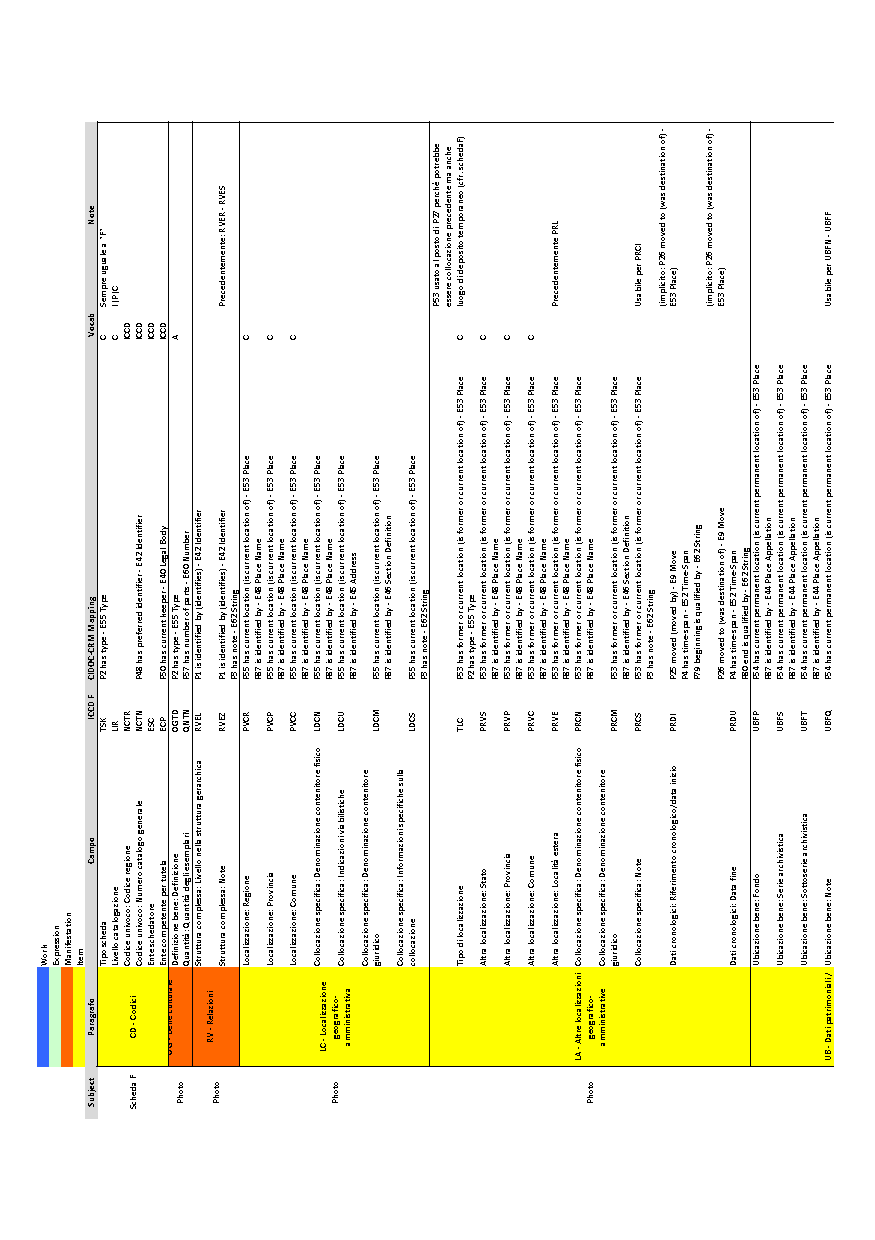
\includegraphics{images/Mapping-v3-1.pdf}
	\caption{Mappatura iniziale - 1}
	\label{fig:mapping-v3-1}
\end{figure}
\begin{figure}[ht!]
    \centering
    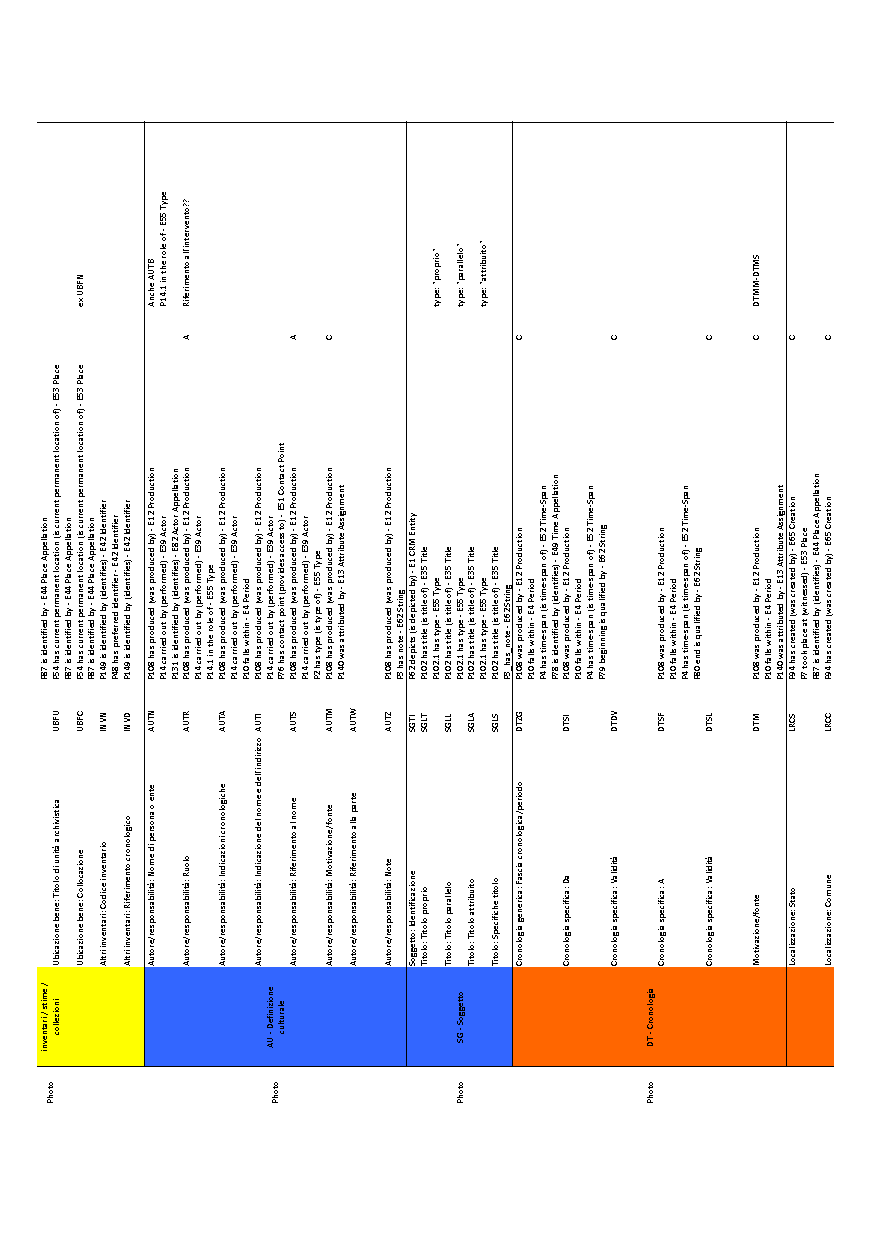
\includegraphics{images/Mapping-v3-2.pdf}
	\caption{Mappatura iniziale - 2}
	\label{fig:mapping-v3-2}
\end{figure}
\begin{figure}[ht!]
    \centering
    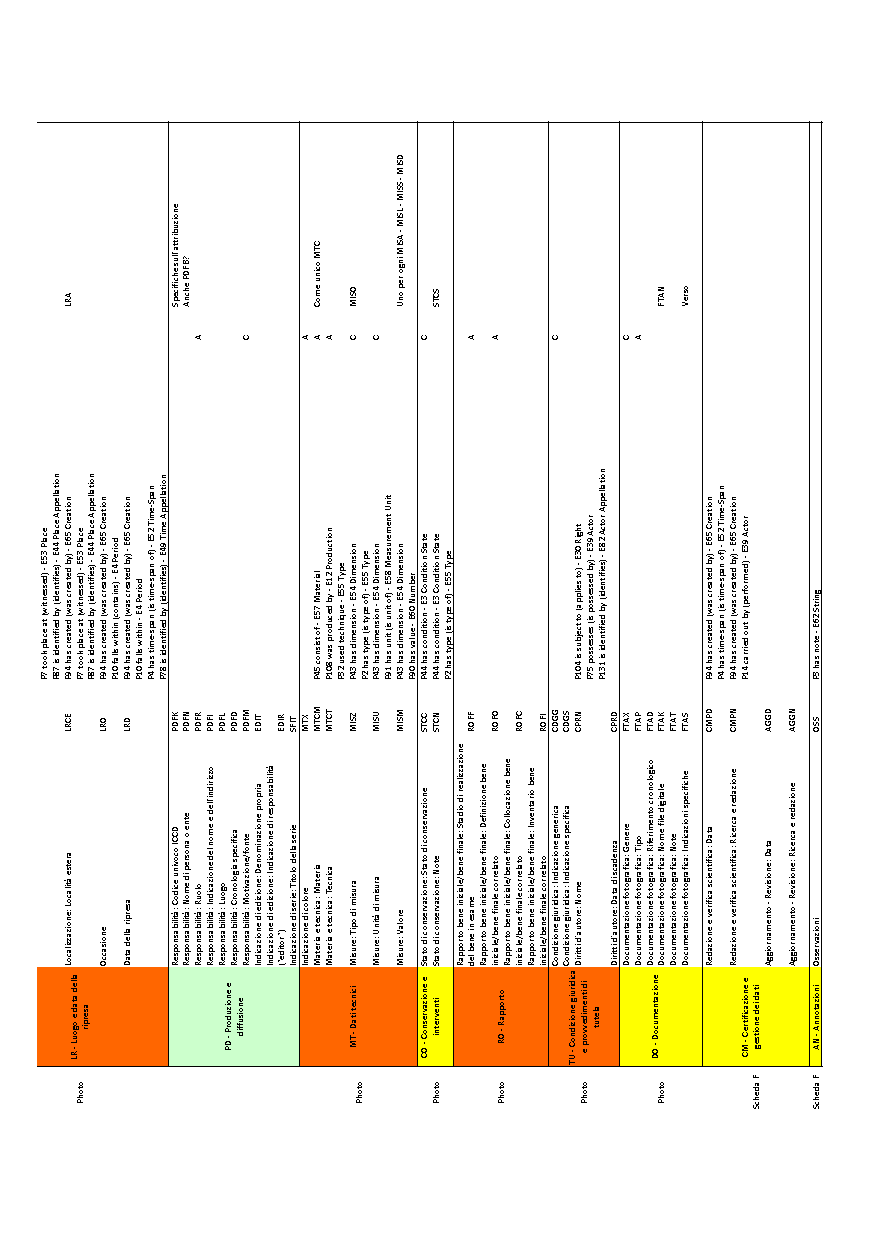
\includegraphics{images/Mapping-v3-3.pdf}
	\caption{Mappatura iniziale - 3}
	\label{fig:mapping-v3-3}
\end{figure}
\end{center}


\chapter{Tracciati}
\rhead[\fancyplain{}{\bfseries \thechapter \:Tracciati}]
{\fancyplain{}{\bfseries\thepage}}

In questa appendice sono riportati i tracciati catalografici originali forniti dalla Fondazione Zeri per la compilazione della Scheda F.

\begin{center}
\tiny

\footnotetext[1]{Campo obbligatorio} \footnotetext[2]{Vocabolario: (c) chiuso / (a) aperto}

\begin{longtable}{ | p{1cm} | p{4cm} | p{.6cm} | p{.6cm} | p{5cm} | }
\caption{Tracciato Scheda F} \label{tab:fzeri-schedaF} \\
\hline \multicolumn{1}{|p{1cm}|}{\cellcolor{lightyellow}\textbf{Codice}} & \multicolumn{1}{p{4cm}|}{\cellcolor{lightyellow}\textbf{Significato}} & \multicolumn{1}{p{.6cm}|}{\cellcolor{lightyellow}\textbf{Obb.\footnotemark[1]}} & \multicolumn{1}{p{.6cm}|}{\cellcolor{lightyellow}\textbf{Voc.\footnotemark[2]}} & \multicolumn{1}{p{5cm}|}{\cellcolor{lightyellow}\textbf{Esempio}} \\ \hline
\endfirsthead
\multicolumn{5}{c}%
{{\bfseries \tablename\ \thetable{} -- continua da pag. precedente}} \\
\hline \multicolumn{1}{|p{1cm}|}{\cellcolor{lightyellow}\textbf{Codice}} & \multicolumn{1}{p{4cm}|}{\cellcolor{lightyellow}\textbf{Significato}} & \multicolumn{1}{p{.6cm}|}{\cellcolor{lightyellow}\textbf{Obb.}} & \multicolumn{1}{p{.6cm}|}{\cellcolor{lightyellow}\textbf{Voc.}} & \multicolumn{1}{p{5cm}|}{\cellcolor{lightyellow}\textbf{Esempio}} \\ \hline
\endhead
\hline \multicolumn{5}{r}{{continua a pag. successiva}}\\
\endfoot
\hline \hline
\endlastfoot
  & Didascalia foto &  &  & Detroit Institute of Arts - Angel Gabriel (in ``Annunciation''). Lorenzo di Niccolò Gerini \\ \hline
  OA-F & Collegamento OA-F & x &  & 2055 \\ \hline
  \multicolumn{5}{|l|}{\cellcolor{lightcyan}CODICI} \\ \hline
  TSK & Tipo scheda & x &  & F \\ \hline
  LIR & Livello ricerca & x & x (c) & I \\ \hline
  NCTR & Codice regione & x & x (c) & 08 \\ \hline
  NCTN & Numero catalogo generale & x &  & 16152 \\ \hline
  ESC & Ente schedatore &  &  & Fondazione Federico Zeri – Università di Bologna \\ \hline
  ECP & Ente competente &  &  &  \\ \hline
  \multicolumn{5}{|l|}{\cellcolor{lightcyan}RELAZIONI}\\ \hline
  RVEL & Livello &  &  &  \\ \hline
  RVER & Codice bene radice &  &  &  \\ \hline
  RVES & Codice bene componente &  &  &  \\ \hline
  OGTI & Oggetto di insieme &  &  &  \\ \hline
  \multicolumn{5}{|l|}{\cellcolor{lightcyan}LOCALIZZAZIONE GEOGRAFICO-AMMINISTRATIVA}\\ \hline
  PVCR & Regione & x &  & Emilia-Romagna \\ \hline
  PVCP & Provincia & x &  & BO \\ \hline
  PVCC & Comune & x &  & Bologna \\ \hline
  LDCN & Denominazione del contenitore & x &  & Ex convento di S. Cristina \\ \hline
  LDCU & Denominazione spazio viabilistico & x &  & piazzetta G. Morandi, 2 \\ \hline
  LDCM & Denominazione della raccolta & x &  & Fototeca Zeri \\ \hline
  LDCS & Specifiche &  &  &  \\ \hline
  \multicolumn{5}{|l|}{\cellcolor{lightcyan}UBICAZIONE}\\ \hline
  UBFP & Fondo & x &  & Fototeca Zeri \\ \hline
  UBFS & Serie archivistica & x &  & Pittura italiana \\ \hline
  UBFN & Numero busta & x &  & 0003 \\ \hline
  UBFT & Intestazione busta & x &  & Pittura italiana sec. XIV. Firenze. Giovanni del Biondo, dipinti maggiori \\ \hline
  UBFF & Numero fascicolo & x &  & 1 \\ \hline
  UBFU & Intestazione fascicolo & x &  & Giovanni del Biondo: dipinti maggiori 1 \\ \hline
  UBFC & Collocazione & x &  & PI\_0051/1/7 \\ \hline
  INVN & Numero inventario generale & x &  & 16152 \\ \hline
  INVD & Data inventariazione &  &  &  \\ \hline
  \multicolumn{5}{|l|}{\cellcolor{lightcyan}ALTRE LOCALIZZAZIONI (paragrafo ripetitivo)}\\ \hline
  TCL & Tipo di localizzazione &  & x (c) & provenienza \\ \hline
  PRVS & Stato &  & x (a) & Italia \\ \hline
  PRVP & Provincia &  & x (a) & FI \\ \hline
  PRVC & Comune &  & x (a) & Firenze \\ \hline
  PRL & Altra località/ Località estera &  &  &  \\ \hline
  PRCD & Denominazione &  & x (a) &  \\ \hline
  PRCM & Denominazione della raccolta &  & x (a) & Collezione privata Sandberg Vavalà Evelyn \\ \hline
  PRCI & Numero di inventario &  &  &  \\ \hline
  PRDI & Data ingresso &  &  &  \\ \hline
  PRDU & Data uscita &  &  &  \\ \hline
  \multicolumn{5}{|l|}{\cellcolor{lightcyan}OGGETTO} \\ \hline
  OGTD & Definizione dell’oggetto & x & x (c) & positivo \\ \hline
  OGTB & Natura biblioteconomica dell’oggetto & x & x (c) & m \\ \hline
  OGTS & Forma specifica dell’oggetto &  & x (a) &  \\ \hline
  QNTN & Numero oggetti/elementi & x &  & 1 \\ \hline
  \multicolumn{5}{|l|}{\cellcolor{lightcyan}SOGGETTO (paragrafo ripetitivo)}\\ \hline
  SGTI & Identificazione del soggetto & x &  & Angelo annunciante - cuspide di polittico \\ \hline
  \multicolumn{5}{|l|}{\cellcolor{lightcyan}TITOLO (paragrafo ripetitivo)}\\ \hline
  SGLT & Titolo proprio & (x) &  & Angel Gabriel (in ``Annunciation''). Lorenzo di Niccolò Gerini \\ \hline
  SGLL & Titolo parallelo &  &  &  \\ \hline
  SGLA & Titolo attribuito & (x) &  &  \\ \hline
  SGLS & Specifiche del titolo & x &  & manoscritto sul verso \\ \hline
  \multicolumn{5}{|l|}{\cellcolor{lightcyan}LUOGO E DATA DELLA RIPRESA}\\ \hline
  LRCS & Stato &  & x (a) &  \\ \hline\
  LRCC & Comune &  & x (a) &  \\ \hline
  LRA & Altra località/località estera &  &  &  \\ \hline
  LRO & Occasione &  &  &  \\ \hline
  LRD & Data &  &  & 1930/ ca. \\ \hline
  \multicolumn{5}{|l|}{\cellcolor{lightcyan}CRONOLOGIA} \\ \hline
  DTZG & Secolo & x & x (c) & XX \\ \hline
  DTSI & Da & x &  & 1929 \\ \hline
  DTSV & Validità &  & x (c) & post \\ \hline
  DTSF & A & x &  & 1950 \\ \hline
  DTSL & Validità &  & x (c) & ante \\ \hline
  DTMM & Motivazione & x & x (a) & analisi storica/ analisi tecnico-formale \\ \hline
  DTMS & Specifiche &  &  &  \\ \hline
  \multicolumn{5}{|l|}{\cellcolor{lightcyan}AUTORE DELLA FOTOGRAFIA (paragrafo ripetitivo)} \\ \hline
  AUFN & Autore della fotografia (autore personale) & (x) &  &  \\ \hline
  AUFB & Autore della fotografia (ente collettivo) & (x) &  & Detroit Institute of Arts \\ \hline
  AUFI & Indicazione del nome e dell’indirizzo &  &  & Photographic Dept. Detroit Institute of Arts \\ \hline
  AUFA & Dati anagrafici/estremi cronologici &  &  &  \\ \hline
  AUFS & Riferimento all’autore &  & x (a) &  \\ \hline
  AUFR & Riferimento all’intervento &  & x (a) &  \\ \hline
  AUFM & Motivazione dell’attribuzione & x & x (a) & timbro \\ \hline
  AUFK & Specifiche sull’attribuzione &  &  &  \\ \hline
  \multicolumn{5}{|l|}{\cellcolor{lightcyan}ALTRO AUTORE (paragrafo ripetitivo)} \\ \hline
  AUTN & Nome scelto (autore personale) &  &  & Giovanni del Biondo \\ \hline
  AUTB & Altro autore (ente collettivo) &  &  & Scuola italiana, scuola toscana, scuola fiorentina \\ \hline
  AUTI & Indicazione del nome &  &  &  \\ \hline
  AUTR & Riferimento all’intervento &  & x (a) &  \\ \hline
  \multicolumn{5}{|l|}{\cellcolor{lightcyan}PRODUZIONE E DIFFUSIONE (paragrafo ripetitivo)} \\ \hline
  PDFN & Nome scelto (personale) &  & x (a) &  \\ \hline
  PDFB & Nome scelto (ente collettivo) &  & x (a) &  \\ \hline
  PDFI & Indicazione del nome e dell’indirizzo &  &  &  \\ \hline
  PDFR & Riferimento al ruolo &  & x (a) &  \\ \hline
  PDFL & Luogo &  &  &  \\ \hline
  PDFD & Data &  &  &  \\ \hline
  PDFM & Motivazione dell’attribuzione &  & x (a) &  \\ \hline
  PDFK & Specifiche sull’attribuzione &  &  &  \\ \hline
  EDIT & Denominazione propria &  &  &  \\ \hline
  EDIR & Indicazione di responsabilità (“editor”) &  &  &  \\ \hline
  SFIT & Titolo della serie &  &  &  \\ \hline
  \multicolumn{5}{|l|}{\cellcolor{lightcyan}RAPPORTO} \\ \hline
  ROFF & Stadio opera &  & x (a) &  \\ \hline
  ROFO & Opera iniziale/finale &  &  &  \\ \hline
  ROFC & Collocazione opera iniziale/finale &  &  &  \\ \hline
  ROFI & Inventario opera iniziale/finale &  &  & 1753 \\ \hline
  \multicolumn{5}{|l|}{\cellcolor{lightcyan}DATI TECNICI} \\ \hline
  MTX & Indicazione di colore & x & x (c) & BN \\ \hline
  MTC & Materia e tecnica & x & x (c) & gelatina ai sali d'argento/ carta baritata \\ \hline
  MISO & Tipo misure & x & x (a) & supporto primario \\ \hline
  MISU & Unità di misura & x & x (c) & mm \\ \hline
  MISA & Altezza & x &  & 227 \\ \hline
  MISL & Larghezza & x &  & 189 \\ \hline
  MISS & Spessore &  &  &  \\ \hline
  MISD & Diametro &  &  &  \\ \hline
  \multicolumn{5}{|l|}{\cellcolor{lightcyan}CONSERVAZIONE} \\ \hline
  STCC & Stato di conservazione &  & x (c) & discreto \\ \hline
  STCS & Indicazioni specifiche &  &  & pieghe \\ \hline
  \multicolumn{5}{|l|}{\cellcolor{lightcyan}CONDIZIONE GIURIDICA} \\ \hline
  CDGG & Indicazione generica &  &  & proprietà Ente pubblico non territoriale \\ \hline
  CDGS & Indicazione specifica &  &  & Alma Mater Studiorum Università di Bologna \\ \hline
  \multicolumn{5}{|l|}{\cellcolor{lightcyan}DIRITTI D’AUTORE} \\ \hline
  CPRN & Nome &  &  &  \\ \hline
  CPRD & Data di scadenza &  &  &  \\ \hline
  \multicolumn{5}{|l|}{\cellcolor{lightcyan}FONTI E DOCUMENTI DI RIFERIMENTO (paragrafo ripetitivo)} \\ \hline
  FTAX & Genere & x & x (c) & allegata \\ \hline
  FTAP & Tipo &  &  & fotografia digitale \\ \hline
  FTAD & Data &  &  &  \\ \hline
  FTAN & Nome del file digitale & x &  & \textbackslash40000\textbackslash16400\textbackslash16152.jpg \\ \hline
  FTAT & Note &  &  & insieme \\ \hline
  Verso & Verso della foto &  & x (c) & pubblico \\ \hline
  \multicolumn{5}{|l|}{\cellcolor{lightcyan}ANNOTAZIONI} \\ \hline
  OSS & Osservazioni &  &  &  \\ \hline
  \multicolumn{5}{|c|}{\cellcolor{lightcyan}COMPILAZIONE} \\ \hline
  CMPD & Data & x &  & 37972 \\ \hline
  CMPN & Nome compilatore & x &  & test \\ \hline
  \multicolumn{5}{|l|}{\cellcolor{lightcyan}AGGIORNAMENTO} \\ \hline
  AGGD & Data & x &  & 37972 \\ \hline
  AGGN & Nome Revisore & x &  & test \\ \hline
\end{longtable}

\newpage

\footnotetext[3]{Campo obbligatorio} \footnotetext[4]{Vocabolario: (c) chiuso / (a) aperto}

\begin{longtable}{ | p{1cm} | p{4cm} | p{.6cm} | p{.6cm} | p{5cm} | }
\caption{Tracciato Scheda OA} \label{tab:fzeri-schedaOA} \\
\hline \multicolumn{1}{|p{1cm}|}{\cellcolor{lightyellow}\textbf{Codice}} & \multicolumn{1}{p{4cm}|}{\cellcolor{lightyellow}\textbf{Significato}} & \multicolumn{1}{p{.6cm}|}{\cellcolor{lightyellow}\textbf{Obb.\footnotemark[3]}} & \multicolumn{1}{p{.6cm}|}{\cellcolor{lightyellow}\textbf{Voc.\footnotemark[4]}} & \multicolumn{1}{p{5cm}|}{\cellcolor{lightyellow}\textbf{Esempio}} \\ \hline
\endfirsthead
\multicolumn{5}{c}%
{{\bfseries \tablename\ \thetable{} -- continua da pag. precedente}} \\
\hline \multicolumn{1}{|p{1cm}|}{\cellcolor{lightyellow}\textbf{Codice}} & \multicolumn{1}{p{4cm}|}{\cellcolor{lightyellow}\textbf{Significato}} & \multicolumn{1}{p{.6cm}|}{\cellcolor{lightyellow}\textbf{Obb.}} & \multicolumn{1}{p{.6cm}|}{\cellcolor{lightyellow}\textbf{Voc.}} & \multicolumn{1}{p{5cm}|}{\cellcolor{lightyellow}\textbf{Esempio}} \\ \hline
\endhead
\hline \multicolumn{5}{r}{{continua a pag. successiva}}\\
\endfoot
\hline \hline
\endlastfoot
  IDC & Identificazione convenzionale & x &  & Giovanni del Biondo - sec. XIV - Angelo annunciante - 2055 \\ \hline
  \multicolumn{5}{|l|}{\cellcolor{lightcyan}CODICI}  \\ \hline
  N. scheda & Numero scheda & x &  & 2055 \\ \hline
  RVEL & Livello &  &  &   \\ \hline
  \multicolumn{5}{|l|}{\cellcolor{lightcyan}UBICAZIONE FOTO DI RIFERIMENTO (paragrafo ripetitivo)}  \\ \hline
  UBFS & Serie  & x & x (a) & Pittura italiana \\ \hline
  UBFN & Numero busta & x & x (a) & 0051 \\ \hline
  UBFF & Numero fascicolo & x & x (a) & 1 \\ \hline
  \multicolumn{5}{|l|}{\cellcolor{lightcyan}AUTORE (paragrafo ripetitivo)}  \\ \hline
  AUTN & Nome & x &  & Giovanni del Biondo \\ \hline
  AUTS & Riferimento all’autore &  & x (c) &  \\ \hline
  ATBD & Ambito culturale & x & x (a) & Scuola italiana, scuola toscana, scuola fiorentina \\ \hline
  AUTM & Motivazione dell’attribuzione & x & x (a) & Classificazione F. Zeri//Bibliografia \\ \hline
  \multicolumn{5}{|l|}{\cellcolor{lightcyan}ALTRE ATTRIBUZIONI (paragrafo ripetitivo)}  \\ \hline
  AAT & Nome altro autore &  &  & Lorenzo di Niccolò  \\ \hline
  AATS & Riferimento all’altro autore &  & x (c) &   \\ \hline
  AATM & Motivazione dell’attribuzione &  & x (a) & Nota anonima sul verso della fotografia  \\ \hline
  \multicolumn{5}{|l|}{\cellcolor{lightcyan}RIFERIMENTO AD ALTRE SCHEDE}  \\ \hline
  RSEC & Oggetto di insieme &  &  & Polittico smembrato di Giovanni del Biondo per l'Oratorio di S. Maria delle Grazie a San Giovanni Valdarno  \\ \hline
  \multicolumn{5}{|l|}{\cellcolor{lightcyan}OGGETTO}  \\ \hline
  OGTD & Definizione & x & x (a) & cuspide di polittico  \\ \hline
  OGTV & Identificazione &  & x (a) & elemento d'insieme  \\ \hline
  OGTT & Tipologia & x & x (c) & dipinto  \\ \hline
  \multicolumn{5}{|l|}{\cellcolor{lightcyan}SOGGETTO  (paragrafo ripetitivo)}  \\ \hline
  SGTI & Titolo & x & x (a) & Adorazione dei pastori  \\ \hline
  SGTT & Denominazione/titolo tradizionale &  &  &   \\ \hline
  \multicolumn{5}{|l|}{\cellcolor{lightcyan}MATERIA E TECNICA (paragrafo ripetitivo)}  \\ \hline
  MTC & Materia e tecnica &  & x (a) & Angelo annunciante  \\ \hline
  \multicolumn{5}{|l|}{\cellcolor{lightcyan}MISURE} \\ \hline
  MISU & Unità di misura &  & x (c) & cm  \\ \hline
  MISA & Altezza &  &  & 35.5  \\ \hline
  MISL & Larghezza &  &  & 17.8  \\ \hline
  MISP & Profondità &  &  &   \\ \hline
  MISD & Diametro &  &  &   \\ \hline
  MISV & Varie &  &  &   \\ \hline
  \multicolumn{5}{|l|}{\cellcolor{lightcyan}RAPPORTO OPERA FINALE/ORIGINALE}  \\ \hline
  ROFF & Stadio opera &  & x (a) &   \\ \hline
  ROFO & Opera finale/originale &  &  &   \\ \hline
  ROFS & Soggetto opera finale/originale &  & x (a) &   \\ \hline
  ROFA & Autore opera finale/originale &  &  &   \\ \hline
  ROFD & Datazione opera finale/originale &  &  &   \\ \hline
  ROFC & Collocazione opera finale/originale &  &  &   \\ \hline
  \multicolumn{5}{|l|}{\cellcolor{lightcyan}LOCALIZZAZIONE GEOGRAFICO-AMMINISTRATIVA} \\ \hline
  PVCS & Stato &  & x (a) & Stati Uniti d'America  \\ \hline
  PVCR & Regione/ Stato federale &  & x (a) & Michigan  \\ \hline
  PVCP & Provincia &  & x (c) &   \\ \hline
  PVCC & Comune &  & x (a) & Detroit (MI)  \\ \hline
  PVCL & Località &  & x (a) &   \\ \hline
  LDCN & Denominazione del contenitore &  & x (a) & Detroit Institute of Arts  \\ \hline
  LDCS & Localizzazione specifica &  &  & Acc. No. 29.315  \\ \hline
  \multicolumn{5}{|l|}{\cellcolor{lightcyan}ALTRE LOCALIZZAZIONI (paragrafo ripetitivo)}  \\ \hline
  PRVS & Stato &  & x (a) & Italia  \\ \hline
  PRVR & Regione &  & x (a) & Toscana  \\ \hline
  PRVP & Provincia &  & x (c) & FI  \\ \hline
  PRVC & Comune &  & x (a) & Firenze  \\ \hline
  PRVL & Località &  & x (a) &   \\ \hline
  PRCD & Denominazione del contenitore &  & x (a) & L. Grassi  \\ \hline
  PRCS & Localizzazione specifica &  &  &   \\ \hline
  PRDI & Data ingresso &  &  &   \\ \hline
  PRDU & Data uscita &  &  & 1929  \\ \hline
  \multicolumn{5}{|l|}{\cellcolor{lightcyan}CRONOLOGIA (paragrafo ripetitivo)} \\ \hline
  DTZG & Indicazione generica & x &  & sec. XIV  \\ \hline
  DTZS & Frazione di secolo &  & x (c) & terzo quarto  \\ \hline
  DTSI & Da & x &  & 1365  \\ \hline
  DTSV & Validità &  & x (c) &   \\ \hline
  DTSF & A & x &  & 1370  \\ \hline
  DTSL & Validità &  & x (c) &   \\ \hline
  \multicolumn{5}{|l|}{\cellcolor{lightcyan}ALTRE DATAZIONI (pragrafo ripetitivo)} \\ \hline
  ADT & Altre datazioni &  &  & sec. XV (1400-1449)  \\ \hline
  \multicolumn{5}{|l|}{\cellcolor{lightcyan}ICONCLASS} \\ \hline
  DESI & Codice Iconclass &  &  &   \\ \hline
  DESS & Indicazioni sul soggetto &  &  & Angelo  \\ \hline
  \multicolumn{5}{|l|}{\cellcolor{lightcyan}BIBLIOGRAFIA (paragrafo ripetitivo)} \\ \hline
  BIBX & Genere &  & x (c) & bibliografia specifica  \\ \hline
  BIBA & Autore &  &  & Berenson B.  \\ \hline
  BIBG & Libro/ Rivista &  &  & Italian Pictures of the Renaissance  \\ \hline
  BIBT & Titolo contributo &  &  &   \\ \hline
  BIBD & Anno di edizione &  &  & 1932  \\ \hline
  BIBN & Pagine specifiche &  &  & p. 240  \\ \hline
  \multicolumn{5}{|l|}{\cellcolor{lightcyan}ALLEGATI (paragrafo ripetitivo)} \\ \hline
  FNTI & Codice identificativo &  &  & F134  \\ \hline
  FNTP & Tipo &  &  & lettera  \\ \hline
  FNTA & Autore &  &  & Contini Bonacossi A.  \\ \hline
  FNTT & Denominazione &  &  & Lettera dattiloscritta di Alessandro Contini Bonacossi a Federico Zeri contenente considerazioni sui due ``Profeti'' di Giovanni del Biondo già parte del polittico dell'Oratorio di S. Maria delle Grazie a San Giovanni Valdarno, transitati dalla Collezione Kress e ora al Museo de Arte de Ponce.  \\ \hline
  FNTD & Data &  &  & 1963/08/02  \\ \hline
  FNTS & Segnatura &  &  & PI\_0051/1/1-13  \\ \hline
  \multicolumn{5}{|l|}{\cellcolor{lightcyan}MOSTRE (Paragrafo ripetitivo)} \\ \hline
  MSTT & Titolo &  &  &   \\ \hline
  MSTL & Luogo &  &  &   \\ \hline
  MSTD & Data &  &  &   \\ \hline
  \multicolumn{5}{|l|}{\cellcolor{lightcyan}OSSERVAZIONI} \\ \hline
  OSS & Osservazioni &  &  & Foto INVN 16152, verso: note anonime a matita in alto: ``Angel Gabriel / (in ``Annunciation'') / Lorenzo di Niccolo Gerini''; in alto a destra: ``Vavalà''  \\ \hline
  NOTE &  &  &  &   \\ \hline
  NOTE & Note &  &  &   \\ \hline
  \multicolumn{5}{|l|}{\cellcolor{lightcyan}FOTO ALLEGATE (paragrafo ripetitivo)} \\ \hline
  FTAP & Tipo &  & x (c) & fotografia digitale  \\ \hline
  FTAD & Data &  &  &   \\ \hline
  FTAN & Nome file digilate &  &  & \textbackslash40000\textbackslash16400\textbackslash16152.jpg  \\ \hline
  FTAT & Note &  &  & insieme  \\ \hline
  Verso & Verso della foto &  & x (c) & Pubblico  \\ \hline
\end{longtable}

\footnotetext[5]{Campo ripetibile} \footnotetext[6]{Campo obbligatorio} \footnotetext[7]{Vocabolario: (c) chiuso / (a) aperto}

\begin{longtable}{ | p{1cm} | p{4cm} | p{.6cm} | p{.6cm} | p{.6cm} | p{5cm} | }
\caption{Tracciato archivio: descrizione archivio} \label{tab:fzeri-archivio-desc} \\
\hline \multicolumn{1}{|p{1cm}|}{\cellcolor{lightyellow}\textbf{Codice}} & \multicolumn{1}{p{4cm}|}{\cellcolor{lightyellow}\textbf{Significato}} & \multicolumn{1}{p{.6cm}|}{\cellcolor{lightyellow}\textbf{Rep.\footnotemark[5]}} & \multicolumn{1}{p{.6cm}|}{\cellcolor{lightyellow}\textbf{Obb.\footnotemark[6]}} & \multicolumn{1}{p{.6cm}|}{\cellcolor{lightyellow}\textbf{Voc.\footnotemark[7]}} & \multicolumn{1}{p{5cm}|}{\cellcolor{lightyellow}\textbf{Esempio}} \\ \hline
\endfirsthead
\multicolumn{6}{c}%
{{\bfseries \tablename\ \thetable{} -- continua da pag. precedente}} \\
\hline \multicolumn{1}{|p{1cm}|}{\cellcolor{lightyellow}\textbf{Codice}} & \multicolumn{1}{p{4cm}|}{\cellcolor{lightyellow}\textbf{Significato}} & \multicolumn{1}{p{.6cm}|}{\cellcolor{lightyellow}\textbf{Rep.\footnotemark[5]}} & \multicolumn{1}{p{.6cm}|}{\cellcolor{lightyellow}\textbf{Obb.\footnotemark[6]}} & \multicolumn{1}{p{.6cm}|}{\cellcolor{lightyellow}\textbf{Voc.\footnotemark[7]}} & \multicolumn{1}{p{5cm}|}{\cellcolor{lightyellow}\textbf{Esempio}} \\ \hline
\endhead
\hline \multicolumn{6}{r}{{continua a pag. successiva}}\\
\endfoot
\hline \hline
\endlastfoot
   Archivio & Archivio &  & x &  & Fondazione Federico Zeri - Università di Bologna \\ \hline
   UBFP & Fondo &  & x & x (a) & Fototeca Zeri \\ \hline
   UBFS & Serie &  & x & x (a) & Pittura italiana \\ \hline
   UBFN & Numero busta &  & x & x (a) & 0051 \\ \hline
   UBFT & Intestazione busta &  & x & x (a) & Pittura italiana sec. XIV. Firenze. Giovanni del Biondo, dipinti maggiori \\ \hline
   UBFF & Numero fascicolo &  & x & x (a) & 1 \\ \hline
   UBFU & Intestazione fascicolo &  & x & x (a) & Giovanni del Biondo: dipinti maggiori 1 \\ \hline
   Consistenza & Consistenza del fascicolo (foto) &  & x &  & 58 \\ \hline
   Consistenza & Consistenza del fascicolo (allegati) &  &  &  & 9 \\ \hline
\end{longtable}

\begin{longtable}{ | p{1cm} | p{4cm} | p{.6cm} | p{.6cm} | p{.6cm} | p{5cm} | }
\caption{Tracciato archivio: autori opere} \label{tab:fzeri-archivio-aut} \\
\hline \multicolumn{1}{|p{1cm}|}{\cellcolor{lightyellow}\textbf{Codice}} & \multicolumn{1}{p{4cm}|}{\cellcolor{lightyellow}\textbf{Significato}} & \multicolumn{1}{p{.6cm}|}{\cellcolor{lightyellow}\textbf{Rep.\footnotemark[5]}} & \multicolumn{1}{p{.6cm}|}{\cellcolor{lightyellow}\textbf{Obb.\footnotemark[6]}} & \multicolumn{1}{p{.6cm}|}{\cellcolor{lightyellow}\textbf{Voc.\footnotemark[7]}} & \multicolumn{1}{p{5cm}|}{\cellcolor{lightyellow}\textbf{Esempio}} \\ \hline
\endfirsthead
\multicolumn{6}{c}%
{{\bfseries \tablename\ \thetable{} -- continua da pag. precedente}} \\
\hline \multicolumn{1}{|p{1cm}|}{\cellcolor{lightyellow}\textbf{Codice}} & \multicolumn{1}{p{4cm}|}{\cellcolor{lightyellow}\textbf{Significato}} & \multicolumn{1}{p{.6cm}|}{\cellcolor{lightyellow}\textbf{Rep.\footnotemark[5]}} & \multicolumn{1}{p{.6cm}|}{\cellcolor{lightyellow}\textbf{Obb.\footnotemark[6]}} & \multicolumn{1}{p{.6cm}|}{\cellcolor{lightyellow}\textbf{Voc.\footnotemark[7]}} & \multicolumn{1}{p{5cm}|}{\cellcolor{lightyellow}\textbf{Esempio}} \\ \hline
\endhead
\hline \multicolumn{6}{r}{{continua a pag. successiva}}\\
\endfoot
\hline \hline
\endlastfoot
   AUTH & Sigla per citazione &  & x &  & 10005477 \\ \hline
   AUTQ & Qualifica &  &  &  & pittore \\ \hline
   AUTN & Autore &  & x &  & Giovanni del Biondo \\ \hline
   AUTA & Dati anagrafici &  & x &  & notizie dal 1356/ 1398 \\ \hline
   AUTC & Cognome &  &  &  &  \\ \hline
   AUTO & Nome &  &  &  & Giovanni \\ \hline
   AUTP & Pseudonimo &  &  &  &  \\ \hline
   AUTE & Nome convenzionale &  &  &  &  \\ \hline
   AUTZ & Sesso &  &  & x (c) &  \\ \hline
   AUTV & Varianti &  &  &  & Giovanni dei Landini (?)/ Maestro della Cappella Rinuccini \\ \hline
   AUTG & Luogo e/o periodo di attività &  &  &  &  \\ \hline
   AUTU & Scuola di appartenenza &  &  &  & scuola fiorentina \\ \hline
   AUTL & Luogo di nascita &  &  &  & Pratovecchio \\ \hline
   AUTD & Data di nascita &  &  &  &  \\ \hline
   AUTX & Luogo di morte &  &  &  & Firenze \\ \hline
   AUTT & Data di morte &  &  &  & 1398 \\ \hline
\end{longtable}

\begin{longtable}{ | p{1cm} | p{4cm} | p{.6cm} | p{.6cm} | p{.6cm} | p{5cm} | }
\caption{Tracciato archivio: bibliografia} \label{tab:fzeri-archivio-biblio} \\
\hline \multicolumn{1}{|p{1cm}|}{\cellcolor{lightyellow}\textbf{Codice}} & \multicolumn{1}{p{4cm}|}{\cellcolor{lightyellow}\textbf{Significato}} & \multicolumn{1}{p{.6cm}|}{\cellcolor{lightyellow}\textbf{Rep.\footnotemark[5]}} & \multicolumn{1}{p{.6cm}|}{\cellcolor{lightyellow}\textbf{Obb.\footnotemark[6]}} & \multicolumn{1}{p{.6cm}|}{\cellcolor{lightyellow}\textbf{Voc.\footnotemark[7]}} & \multicolumn{1}{p{5cm}|}{\cellcolor{lightyellow}\textbf{Esempio}} \\ \hline
\endfirsthead
\multicolumn{6}{c}%
{{\bfseries \tablename\ \thetable{} -- continua da pag. precedente}} \\
\hline \multicolumn{1}{|p{1cm}|}{\cellcolor{lightyellow}\textbf{Codice}} & \multicolumn{1}{p{4cm}|}{\cellcolor{lightyellow}\textbf{Significato}} & \multicolumn{1}{p{.6cm}|}{\cellcolor{lightyellow}\textbf{Rep.\footnotemark[5]}} & \multicolumn{1}{p{.6cm}|}{\cellcolor{lightyellow}\textbf{Obb.\footnotemark[6]}} & \multicolumn{1}{p{.6cm}|}{\cellcolor{lightyellow}\textbf{Voc.\footnotemark[7]}} & \multicolumn{1}{p{5cm}|}{\cellcolor{lightyellow}\textbf{Esempio}} \\ \hline
\endhead
\hline \multicolumn{6}{r}{{continua a pag. successiva}}\\
\endfoot
\hline \hline
\endlastfoot
   BIBH & Sigla per citazione &  & x &  &  \\ \hline
   BIBA & Autore &  & x &  & Berenson B. \\ \hline
   BIBC & Curatore &  &  &  &  \\ \hline
   BIBF & Tipo &  &  &  & monografia \\ \hline
   BIBG & Libro/rivista &  & x &  & Italian Pictures of the Renaissance \\ \hline
   BIBT & Titolo contributo &  &  &  &  \\ \hline
   BIBL & Luogo di edizione &  &  &  & Oxford \\ \hline
   BIBZ & Editore &  &  &  & Clarendon Press \\ \hline
   BIBD & Anno di edizione &  &  &  & 1932 \\ \hline
   BIBE & Numero di edizione &  &  &  &  \\ \hline
   BIBS & Specifiche &  &  &  &  \\ \hline
   BIBV & Volume &  &  &  &  \\ \hline
   BIBP & Pagine &  &  &  &  \\ \hline
\end{longtable}

\begin{longtable}{ | p{1cm} | p{4cm} | p{.6cm} | p{.6cm} | p{.6cm} | p{5cm} | }
\caption{Tracciato archivio: allegati} \label{tab:fzeri-archivio-attach} \\
\hline \multicolumn{1}{|p{1cm}|}{\cellcolor{lightyellow}\textbf{Codice}} & \multicolumn{1}{p{4cm}|}{\cellcolor{lightyellow}\textbf{Significato}} & \multicolumn{1}{p{.6cm}|}{\cellcolor{lightyellow}\textbf{Rep.\footnotemark[5]}} & \multicolumn{1}{p{.6cm}|}{\cellcolor{lightyellow}\textbf{Obb.\footnotemark[6]}} & \multicolumn{1}{p{.6cm}|}{\cellcolor{lightyellow}\textbf{Voc.\footnotemark[7]}} & \multicolumn{1}{p{5cm}|}{\cellcolor{lightyellow}\textbf{Esempio}} \\ \hline
\endfirsthead
\multicolumn{6}{c}%
{{\bfseries \tablename\ \thetable{} -- continua da pag. precedente}} \\
\hline \multicolumn{1}{|p{1cm}|}{\cellcolor{lightyellow}\textbf{Codice}} & \multicolumn{1}{p{4cm}|}{\cellcolor{lightyellow}\textbf{Significato}} & \multicolumn{1}{p{.6cm}|}{\cellcolor{lightyellow}\textbf{Rep.\footnotemark[5]}} & \multicolumn{1}{p{.6cm}|}{\cellcolor{lightyellow}\textbf{Obb.\footnotemark[6]}} & \multicolumn{1}{p{.6cm}|}{\cellcolor{lightyellow}\textbf{Voc.\footnotemark[7]}} & \multicolumn{1}{p{5cm}|}{\cellcolor{lightyellow}\textbf{Esempio}} \\ \hline
\endhead
\hline \multicolumn{6}{r}{{continua a pag. successiva}}\\
\endfoot
\hline \hline
\endlastfoot
   \multicolumn{6}{|l|}{\cellcolor{lightcyan}PROVENIENZA}  \\ \hline
   FNTN & Nome Archivio/ Fondo &  & x &  & Fondazione Federico Zeri - Università di Bologna/ Fototeca Zeri \\ \hline
   UBFP & Fondo &  & x &  & Fototeca  Zeri \\ \hline
   UBFS & Serie &  & x &  & Pittura italiana \\ \hline
   UBFN & Numero busta &  & x &  & 0051 \\ \hline
   UBFT & Intestazione busta &  & x &  & Pittura italiana sec. XIV. Firenze. Giovanni del Biondo, dipinti maggiori \\ \hline
   UBFF & Numero fascicolo &  & x &  & 1 \\ \hline
   UBFU & Intestazione fascicolo &  & x &  & Giovanni del Biondo: dipinti maggiori 1 \\ \hline
   FNTS & Segnatura &  & x &  & PI\_0051/1/1-13 \\ \hline
   N. BID & Numero identificativo (BID) del volume collegato al documento &  &  &  &  \\ \hline
   N. Scheda OA & Numero scheda dell’opera d’arte collegata al documento & Si &  &  & 2054 \\ \hline
   \multicolumn{6}{|l|}{\cellcolor{lightcyan}ATTUALE COLLOCAZIONE}  \\ \hline
   FNTO & Collocazione &  &  &  & Allegati Fototeca 3 \\ \hline
   FNTI & Codice identificativo &  & x &  & F134 \\ \hline
   FNTF & Consistenza &  &  &  & 1 \\ \hline
   \multicolumn{6}{|l|}{\cellcolor{lightcyan}TIPOLOGIA E CONTENUTO}  \\ \hline
   FNTP & Tipo &  &  & x (a) & lettera \\ \hline
   FNTA & Autore &  &  &  & Contini Bonacossi A. \\ \hline
   FNTE & Destinatario &  &  &  & Zeri F. \\ \hline
   FNTD & Data &  &  &  & 1963/08/02 \\ \hline
   FNTT & Descrizione &  & x &  & Lettera dattiloscritta di Alessandro Contini Bonacossi a Federico Zeri contenente considerazioni sui due ``Profeti'' di Giovanni del Biondo già parte del polittico dell'Oratorio di S. Maria delle Grazie a San Giovanni Valdarno, transitati dalla Collezione Kress e ora al Museo de Arte de Ponce. \\ \hline
   FNTR & Trascrizione &  &  &  &  \\ \hline
   \multicolumn{6}{|l|}{\cellcolor{lightcyan}IMMAGINI E VISIBILITÀ}  \\ \hline
   FNTJ & Collegamento al file digitale & Si &  &  & \textbackslash{}Allegati\textbackslash{}Fototeca\textbackslash{}f134\_g.jpg \\ \hline
   Pubblico/Privato & Pubblico/ Privato &  &  &  & privato \\ \hline
\end{longtable}

\footnotetext[5]{Campo ripetibile} \footnotetext[6]{Campo obbligatorio} \footnotetext[7]{Vocabolario: (c) chiuso / (a) aperto}

\begin{longtable}{ | p{1cm} | p{4cm} | p{.6cm} | p{.6cm} | p{.6cm} | p{5cm} | }
\caption{Tracciato archivio: autori fotografi} \label{tab:fzeri-archivio-ph} \\
\hline \multicolumn{1}{|p{1cm}|}{\cellcolor{lightyellow}\textbf{Codice}} & \multicolumn{1}{p{4cm}|}{\cellcolor{lightyellow}\textbf{Significato}} & \multicolumn{1}{p{.6cm}|}{\cellcolor{lightyellow}\textbf{Rep.\footnotemark[5]}} & \multicolumn{1}{p{.6cm}|}{\cellcolor{lightyellow}\textbf{Obb.\footnotemark[6]}} & \multicolumn{1}{p{.6cm}|}{\cellcolor{lightyellow}\textbf{Voc.\footnotemark[7]}} & \multicolumn{1}{p{5cm}|}{\cellcolor{lightyellow}\textbf{Esempio}} \\ \hline
\endfirsthead
\multicolumn{6}{c}%
{{\bfseries \tablename\ \thetable{} -- continua da pag. precedente}} \\
\hline \multicolumn{1}{|p{1cm}|}{\cellcolor{lightyellow}\textbf{Codice}} & \multicolumn{1}{p{4cm}|}{\cellcolor{lightyellow}\textbf{Significato}} & \multicolumn{1}{p{.6cm}|}{\cellcolor{lightyellow}\textbf{Rep.\footnotemark[5]}} & \multicolumn{1}{p{.6cm}|}{\cellcolor{lightyellow}\textbf{Obb.\footnotemark[6]}} & \multicolumn{1}{p{.6cm}|}{\cellcolor{lightyellow}\textbf{Voc.\footnotemark[7]}} & \multicolumn{1}{p{5cm}|}{\cellcolor{lightyellow}\textbf{Esempio}} \\ \hline
\endhead
\hline \multicolumn{6}{r}{{continua a pag. successiva}}\\
\endfoot
\hline \hline
\endlastfoot
   AUFH & Sigla per citazione &  &  &  & 10002303 \\ \hline
   AUFQ & Qualifica &  &  &  &  \\ \hline
   AUFN/ AUFB & Autore della foto (personale/ collettivo) &  & x &  & Detroit Institute of Arts \\ \hline
   AUFC & Cognome &  &  &  &  \\ \hline
   AUFO & Nome &  &  &  &  \\ \hline
   AUFP & Pseudonimo &  &  &  &  \\ \hline
   AUFJ & Nazionalità &  &  &  & Statunitense \\ \hline
   AUFZ & Sesso &  &  &  &  \\ \hline
   AUFV & Varianti &  &  &  &  \\ \hline
   AUFG & Luogo e/o periodo di attività &  &  &  & Detroit (Michigan), 5200 Woodward Avenue (1885 - ) \\ \hline
   AUFW & Luoghi conservazione raccolte &  &  &  &  \\ \hline
   AUFL & Luogo di nascita &  &  &  &  \\ \hline
   AUFD & Data di nascita &  &  &  &  \\ \hline
   AUFX & Luogo di morte &  &  &  &  \\ \hline
   AUFT & Data di morte &  &  &  &  \\ \hline
\end{longtable}
\end{center}
\footnotetext[5]{Campo ripetibile} \footnotetext[6]{Campo obbligatorio} \footnotetext[7]{Vocabolario: (c) chiuso / (a) aperto}


\chapter{Campi del dataset Zeri effettivamente in uso}
\rhead[\fancyplain{}{\bfseries \thechapter \:Campi del dataset Zeri effettivamente in uso}]
{\fancyplain{}{\bfseries\thepage}}

Durante l'analisi degli XML in input si è reso necessario avere un'istantanea della situazione reale, ovvero dei paragrafi e dei campi effettivamente utilizzati e della loro struttura per come traspariva dal dump XML; affidarsi all'analisi del singolo record non era fattibile in quanto non necessariamente in un dato record vengono compilati tutti i campi, alcuni dei quali sono per giunta mutualmente esclusivi tra di loro.

È stato quindi scritto un programma (\texttt{schema\_builder.py}) che effettuasse il parsing di tutto l'XML in input e ne costruisse un record fasullo contenente ogni campo in uso nell'intero dataset, contenente ovviamente informazioni incoerenti all'interno dello stesso record ma utile per la revisione della struttura e la scrittura dell'algoritmo di parsing del dataset.

\lstinputlisting[caption=Elenco di tutti i campi effettivamente in uso nel dataset XML fornito dalla Fondazione Zeri e loro possibile valore, label=listing:fzeri-fakerecord]{../zerielode/catalog_schema.txt}


\chapter{Esempio di conversione}
\rhead[\fancyplain{}{\bfseries \thechapter \:Esempio di conversione}]
{\fancyplain{}{\bfseries\thepage}}

In questa appendice è riportata la conversione reale applicata ad un record di esempio tratto dall'archivio Zeri in XML.

\lstinputlisting[language=XML, caption=Esempio di record dell'archivio Zeri in XML, label=listing:sample-source]{../zerielode/catalog/fzeri_F_2014_03_11_163504_single.xml}

\lstinputlisting[caption=Esempio di conversione del record \ref{listing:sample-source} in formato Turtle, label=listing:sample-output]{../zerielode/single.ttl}



\begin{thebibliography}{90}
\rhead[\fancyplain{}{\bfseries \leftmark}]{\fancyplain{}{\bfseries
\thepage}}

\addcontentsline{toc}{chapter}{\numberline{}{Bibliografia}}

\bibitem[BER 2006]{4} Berners-Lee, T. \emph{Linked data.} 2006, ultimo agg. June 18, 2009.\\
\url{http://www.w3.org/DesignIssues/LinkedData.html}

\bibitem[BER 2007]{3} Berners-Lee, T. \emph{Giant Global Graph}. In Decentralized Information Group, 21 November 2007.\\
\url{http://dig.csail.mit.edu/breadcrumbs/node/215}

\bibitem[CDG 2011]{13} Crofts, N., Doerr, M., Gill, T., Stead, S., Stiff, M. \emph{Definition of the CIDOC Conceptual Reference Model.} Version 5.0.4 (November 2011). ICOM/CIDOC CRM Special Interest Group.\\
\url{http://www.cidoc-crm.org/docs/cidoc_crm_version_5.0.4.pdf}

\bibitem[DKG 2011]{7} Damova, M., Kiryakov, A. Grinberg, M., Bergman, M., Giasson, F., Simov, K. \emph{Creation and Integration of Reference Ontologies for Efficient LOD Management.} In: Semi-Automatic Ontology Development: Processes and Resources, IGI Global, Hershey PA, USA, 2011.

\bibitem[DL190/1999]{16} DECRETO LEGISLATIVO 29 ottobre 1999, n. 490 - \emph{Testo unico delle disposizioni legislative in materia di beni culturali e ambientali}, a norma dell'articolo 1 della legge 8 ottobre 1997, n. 352.\\
\url{http://www.normattiva.it/uri-res/N2Ls?urn:nir:stato:decreto.legislativo:1999;490}

\bibitem[DOE 2010]{10} Doerr, M. (2010). \emph{The Europeana Data Model (EDM) mapping to CIDOC-CRM.}\\
\url{http://www.cidoc-crm.org/docs/CRM-EDM_FRBR.ppt}

\bibitem[DWG 2012]{9} De Boer V., Wielemaker J., Gent van J., Hildebrand M., Isaac A., Ossenbruggen van J., Schreiber G. (2012) \emph{Supporting Linked Data Production for Cultural Heritage Institutes: The Amsterdam Museum Case Study.} The Semantic Web: Research and Applications. LNCS Vol. 7295, pp 733-747.

\bibitem[ELL 2013]{5} Edelstein, L.G.a, Li-Madeo C., Marden J., Rhonemus A., Whysel N. (Spring 2013). \emph{Linked Open Data for Cultural Heritage: Evolution of an Information Technology.}\\
\url{http://www.whysel.com/papers/LIS670-Linked-Open-Data-for-Cultural-Heritage.pdf}

\bibitem[EDM]{11} EDM (Europeana Data Model). Documentation: \url{http://pro.europeana.eu/edm-documentation}

\bibitem[FGJ 1997]{26} Fernández-López, M., Gómez-Pérez, A. and Juristo, N. (1997). \emph{Methontology: From Ontological Art Towards Ontological Engineering.} In Proceedings of the 1997 AAAI Spring Symposium, SS-97-06: 33–40. Menlo Park, California, USA: AAAI Press. Retrieved from http://www.aaai.org/Papers/Symposia/Spring/1997/SS-97-06/SS97-06-005.pdf

\bibitem[FRBR]{19} FRBR (Functional Requirements for Bibliographic Records).\\
\url{http://www.ifla.org/publications/functional-requirements-for-bibliographic-records}

\bibitem[FRBR-CRM]{20} FRBR-CRM, FRBRoo.\\
\url{http://www.cidoc-crm.org/frbr_inro.html}

\bibitem[GMP 2014]{29} Gonano C.M., Mambelli F., Peroni S., Tomasi F. and Vitali F. (2014). \emph{Zeri e LODE. Extracting the Zeri photo archive to Linked Open Data: formalizing the conceptual model}. Bologna, 2014.

\bibitem[ICCDFot1999]{14} ICCD (Istituto Centrale per il Catalogo e la Documentazione), \emph{Beni fotografici.} 1999 (agg. 2004).\\
\url{http://www.iccd.beniculturali.it/index.php?it/387/beni-fotografici}

\bibitem[ICCDSto1999]{15} ICCD (Istituto Centrale per il Catalogo e la Documentazione), \emph{Beni storici e artistici.} 1992.\\
\url{http://www.iccd.beniculturali.it/index.php?it/253/beni-storici-e-artistici}

\bibitem[JCB 2011]{21} Jentzsch A. Cyganiak R., Bizer C. \emph{State of the LOD Cloud.} - (Version 0.3, 09/19/2011)\\
\url{http://lod-cloud.net/state/}

\bibitem[LSM 2013]{22} Lebo, T., Sahoo, S. and McGuinness, D. (2013). PROV-O: The PROV Ontology. W3C Recommendation, 30 April 2013. World Wide Web Consortium.\\
\url{http://www.w3.org/TR/prov-o/}

\bibitem[MLW 2013]{23} Marden J., Li-Madeo C., Whysel N., Edelstein J. (2013), \emph{Linked open data for cultural heritage: evolution of an information technology.} Proceeding SIGDOC '13, pp. 107-112. ACM New York, NY, USA.

\bibitem[MPP 2012]{24} Motik, B., Patel-Schneider, P. F. and Parsia, B. (2012). OWL 2 Web Ontology Language: Structural Specification and Functional-Style Syntax (Second Edition). W3C Recommendation, 11 December 2012. World Wide Web Consortium. Retrieved from http://www.w3.org/TR/owl2-syntax/

\bibitem[PCDHN]{25} Pan-Canadian Documentary Heritage Network (PCDHN) Linked Open Data (LOD) Visualization ``Proof-of-Concept''\\
\url{http://www.canadiana.ca/sites/pub.canadiana.ca/files/PC DHN\%20Proof-of-concept_Final-Report-ENG_0.pdf}

\bibitem[PES 2012]{6} Peroni, S. and Shotton, D. (2012). \emph{FaBiO and CiTO: Ontologies for describing bibliographic resources and citations.} Web Semantics: Science, Services and Agents on the World Wide Web, 17: 33–43. DOI: 10.1016/j.websem.2012.08.001

\bibitem[POL 2009]{1} Pollock, Jeffrey T. \emph{Semantic Web For Dummies}. Wiley, 2009. ISBN: 9780470396797.

\bibitem[PSV 2012]{18} Peroni, S., Shotton, D. and Vitali, F. (2012). \emph{Scholarly publishing and linked data: describing roles, statuses, temporal and contextual extents.} In H. Sack and T. Pellegrini (Eds.), Proceedings of i-Semantics 2012: 9– 16. New York, New York, US: ACM Press. DOI: 10.1145/2362499.2362502

\bibitem[PTV 2012]{8} Peroni S., Tomasi F. and Vitali F. (2012). \emph{Reflecting on the Europeana Data Model.} In: IRCDL 2012, pp. 228– 240. Communications in Computer and Information Science (CCIS) 354, Springer, Heidelberg, Germany 2012.

\bibitem[PTV 2013]{17} Peroni S., Tomasi F. and Vitali F. (2013). \emph{The aggregation of heterogeneous metadata in Web-based cultural heritage collections. A case study.} IJWET vol. 8, n. 4, pp. 412-432. ISSN 1476-1289. DOI: 10.154/IJWET.2013.059107

\bibitem[SMN 2013]{12} Scarselli T., Mancinelli M. L., Niccolucci F. (2013). \emph{Mapping ICCD Archaeological Data to CIDOC-CRM: the RA Schema.}\\
\url{http://www.academia.edu/5549957/Mapping_ICCD_arc haeological_data_to_CIDOC-CRM_the_RA_Schema}

\bibitem[USG 1996]{27} Uschold, M. and Gruninger, M. (1996). \emph{Ontologies: principles, methods and applications.} The Knowledge Engineering Review, 11(02): 93–136. DOI: 10.1017/S0269888900007797

\bibitem[VBG 2009]{28} Volz J., Bizer C., Gaedke M., and Kobilarov G. \emph{Discovering and maintaining links on the web of data.} In Proceedings of the 8th International Semantic Web Conference, pp. 650-665, 2009.

\bibitem[W3C2013]{2} W3C Data Activity \emph{W3C Semantic Web Activity Introduction}. Dec 2013.\\
\url{http://www.w3.org/2001/sw/}

\bibitem[ZEL 2006]{30} Zeldman J. emph{Web 3.0} In A List Apart, January 17, 2006.\\
\url{http://alistapart.com/article/web3point0}

\bibitem[SHA 2006]{31} Shannon V. \emph{A `more revolutionary' Web}, in The New York Times, May 23, 2006.\\
\url{http://www.nytimes.com/2006/05/23/technology/23iht-web.html?_r=0}

\end{thebibliography}
\clearpage{\pagestyle{empty}\cleardoublepage}


\pagestyle{plain}

\chapter*{Ringraziamenti}

Ho sempre pensato che la pagina dei ringraziamenti fosse quella più letta in qualsiasi dissertazione di laurea e al contempo quella più difficile da scrivere per la sua disponibilità a raccogliere santi e fanti, le colonne dei buoni e dei cattivi, discorsi seri e faceti, celebrazioni dovute e omaggi inaspettati.

Altresì ho sempre pensato che fosse un modo forse un po' più rilevante di altri per riconoscere l'importanza di chi ha viaggiato con me e di chi lo sta ancora facendo.

E dopo tredici anni i compagni di viaggio passati e presenti cominciano ad essere molti, e c'è sempre il rischio che ne scappi qualcuno.

In rigoroso ordine sparso comincio quindi a ringraziare chi ha condiviso i primi anni di università, il glorioso \emph{Lab1} con gli iMac colorati battezzati come gruppi Metal, il gruppo \emph{BES} capitanato da Re Enzo, Mattia che mi veniva a svegliare entrando dalla finestra e Mauro che mi ha sopportato finché ce l'ha fatta.

Sicuramente un grosso grazie va a Fabio e a Silvio e Francesca per aver accolto a braccia aperte la lucida follia di riaprire la partita, calare le tredici carte e chiudere in una sola mano. Senza di voi probabilmente non ce l'avrei fatta.

Andrea e Alberto sono sempre lì, nell'appartamentino che si sono costruiti da qualche parte in me, nonostante i silenzi e i distacchi. E così Gianluca, così diverso da me da rendere il mio legame con lui irrinunciabile.

Non posso non menzionare \emph{RoART} tutta, le notti passate a organizzare \emph{RO-Woodstock}, le riunioni, i chitarristi sulla camionetta dei pompieri, le foto e la musica. E non posso non rivolgere un pensiero particolare a Enrico e Francesca, loro sanno perché.

A ventisei anni ho scoperto il teatro, le sue gioie e i suoi dolori; \emph{Nexus} ormai è una seconda casa ed è grazie a chi ne fa parte, a chi mi affianca in scena e fuori, che la mia voglia di continuare il cammino cresce sempre più: Demis e Barbara, sapete di averne il merito e la colpa.

\emph{Comperio} è stata la mia università quando ho deciso di abbandonare Bologna, grazie a Dario e Paolo che mi hanno insegnato un lavoro; e un doveroso grazie a Marco, Isacco, Giulio e Nicolò per i confronti, i bisticci, i discorsi e per le innumerevoli puttanate che hanno accompagnato le pause caffè.

Grazie a Matteo per tutte le avventure passate insieme, assieme ad Andrea per le serate da Severo, per le LAN e per i compleanni al cinese.

Grazie ai miei santoli Anna e Gianni per essere sempre stati i miei secondi genitori; a nonna Maria per gli ovetti e per averle fatto venire i capelli bianchi, e a nonna Rina, ché son sicuro che semmai qualcosa esiste, lassù, ogni tanto butta un occhio su di me per merito suo.

Grazie a Sarah per gli anni passati insieme, per le cose buone che ci sono state, nonostante tutto.

Grazie a Cecilia per esserci stata sempre, ogni singola volta in cui sono inciampato, e per il coraggio e la schiettezza che avrei sempre voluto mi fossero d'esempio.

A Silvia, per essere cresciuta con me, per avermi accompagnato negli anni dell'università e in quelli a seguire, per aver toccato il cielo con un dito e per mille e mille altre cose. E per esserci di nuovo, finalmente.

A Sara per avermi raccolto, per essere stata la scintilla che ha riacceso il fuoco, ché senza di lei non sareste a leggere queste parole. Per avermi permesso nuovamente di credere che tutto è possibile.

Grazie a Martina per le furiose litigate e i larghi sorrisi, so che non è stato affatto facile avere un fratello come me.

Grazie a Celeste per un disegno che ancora conservo e che ho riguardato commosso a gennaio.

Ho sempre creduto nell'importanza delle ultime righe, e per questo vanno a chi mi ha permesso di essere quello che sono, a chi mi ha regalato risorse ma soprattutto esperienza, a chi si è scontrato e incontrato con me, a chi è cresciuto assieme a me. A chi credo non abbia mai perso veramente la speranza di vedermi con una corona d'alloro in testa: Paola e Luciano.\\
Sono fiero di essere vostro figlio.

\end{document}

